\documentclass[a4paper]{book}
\usepackage{makeidx}
\usepackage{graphicx}
\usepackage{multicol}
\usepackage{float}
\usepackage{listings}
\usepackage{color}
\usepackage{ifthen}
\usepackage[table]{xcolor}
\usepackage{textcomp}
\usepackage{alltt}
\usepackage{ifpdf}
\ifpdf
\usepackage[pdftex,
            pagebackref=true,
            colorlinks=true,
            linkcolor=blue,
            unicode
           ]{hyperref}
\else
\usepackage[ps2pdf,
            pagebackref=true,
            colorlinks=true,
            linkcolor=blue,
            unicode
           ]{hyperref}
\usepackage{pspicture}
\fi
\usepackage[utf8]{inputenc}
\usepackage[french]{babel}

\usepackage{mathptmx}
\usepackage[scaled=.90]{helvet}
\usepackage{courier}
\usepackage{doxygen}
\lstset{language=C++,inputencoding=utf8,basicstyle=\footnotesize,breaklines=true,breakatwhitespace=true,tabsize=8,numbers=left }
\makeindex
\setcounter{tocdepth}{3}
\renewcommand{\footrulewidth}{0.4pt}
\begin{document}
\hypersetup{pageanchor=false}
\begin{titlepage}
\vspace*{7cm}
\begin{center}
{\Large XMLLib \\[1ex]\large 0.1 }\\
\vspace*{1cm}
{\large Généré par Doxygen 1.7.2}\\
\vspace*{0.5cm}
{\small Fri Apr 15 2011 16:44:38}\\
\end{center}
\end{titlepage}
\clearemptydoublepage
\pagenumbering{roman}
\tableofcontents
\clearemptydoublepage
\pagenumbering{arabic}
\hypersetup{pageanchor=true}
\chapter{Index des espaces de nommage}
\section{Liste des espaces de nommage}
Liste de tous les espaces de nommage avec une brève description:\begin{DoxyCompactList}
\item\contentsline{section}{\hyperlink{namespacexml}{xml} }{\pageref{namespacexml}}{}
\end{DoxyCompactList}

\chapter{Index des classes}
\section{Hiérarchie des classes}
Cette liste d'héritage est classée approximativement par ordre alphabétique :\begin{DoxyCompactList}
\item \contentsline{section}{xml::InterfaceNodeVisitor}{\pageref{classxml_1_1_interface_node_visitor}}{}
\begin{DoxyCompactList}
\item \contentsline{section}{xml::DotOutputVisitor}{\pageref{classxml_1_1_dot_output_visitor}}{}
\item \contentsline{section}{xml::OutputVisitor}{\pageref{classxml_1_1_output_visitor}}{}
\end{DoxyCompactList}
\item \contentsline{section}{xml::Node}{\pageref{classxml_1_1_node}}{}
\begin{DoxyCompactList}
\item \contentsline{section}{xml::MarkupNode}{\pageref{classxml_1_1_markup_node}}{}
\begin{DoxyCompactList}
\item \contentsline{section}{xml::CompositeMarkupNode}{\pageref{classxml_1_1_composite_markup_node}}{}
\end{DoxyCompactList}
\item \contentsline{section}{xml::TextNode}{\pageref{classxml_1_1_text_node}}{}
\end{DoxyCompactList}
\end{DoxyCompactList}

\chapter{Index des classes}
\section{Liste des classes}
Liste des classes, structures, unions et interfaces avec une brève description :\begin{DoxyCompactList}
\item\contentsline{section}{\hyperlink{structdtd_1_1_choice_1_1___state}{dtd::Choice::\_\-State} }{\pageref{structdtd_1_1_choice_1_1___state}}{}
\item\contentsline{section}{\hyperlink{structdtd_1_1_quantifiable_content_1_1___state}{dtd::QuantifiableContent::\_\-State} }{\pageref{structdtd_1_1_quantifiable_content_1_1___state}}{}
\item\contentsline{section}{\hyperlink{structdtd_1_1_sequence_1_1___state}{dtd::Sequence::\_\-State} }{\pageref{structdtd_1_1_sequence_1_1___state}}{}
\item\contentsline{section}{\hyperlink{classdtd_1_1_any_content}{dtd::AnyContent} }{\pageref{classdtd_1_1_any_content}}{}
\item\contentsline{section}{\hyperlink{classdtd_1_1_attribute}{dtd::Attribute} }{\pageref{classdtd_1_1_attribute}}{}
\item\contentsline{section}{\hyperlink{structdtd_1_1_attributes_comparator}{dtd::AttributesComparator} }{\pageref{structdtd_1_1_attributes_comparator}}{}
\item\contentsline{section}{\hyperlink{classdtd_1_1_browsable_content}{dtd::BrowsableContent} }{\pageref{classdtd_1_1_browsable_content}}{}
\item\contentsline{section}{\hyperlink{classdtd_1_1_choice}{dtd::Choice} }{\pageref{classdtd_1_1_choice}}{}
\item\contentsline{section}{\hyperlink{classdtd_1_1_content}{dtd::Content} }{\pageref{classdtd_1_1_content}}{}
\item\contentsline{section}{\hyperlink{classdtd_1_1_d_t_d}{dtd::DTD} }{\pageref{classdtd_1_1_d_t_d}}{}
\item\contentsline{section}{\hyperlink{classdtd_1_1_element_content}{dtd::ElementContent} }{\pageref{classdtd_1_1_element_content}}{}
\item\contentsline{section}{\hyperlink{classdtd_1_1_element_reference}{dtd::ElementReference} }{\pageref{classdtd_1_1_element_reference}}{}
\item\contentsline{section}{\hyperlink{classdtd_1_1_empty_content}{dtd::EmptyContent} }{\pageref{classdtd_1_1_empty_content}}{}
\item\contentsline{section}{\hyperlink{classdtd_1_1_interface_d_t_d_visitor}{dtd::InterfaceDTDVisitor} }{\pageref{classdtd_1_1_interface_d_t_d_visitor}}{}
\item\contentsline{section}{\hyperlink{classdtd_1_1_mixed_content}{dtd::MixedContent} }{\pageref{classdtd_1_1_mixed_content}}{}
\item\contentsline{section}{\hyperlink{classdtd_1_1_optional_content}{dtd::OptionalContent} }{\pageref{classdtd_1_1_optional_content}}{}
\item\contentsline{section}{\hyperlink{classdtd_1_1_output_d_t_d_visitor}{dtd::OutputDTDVisitor} }{\pageref{classdtd_1_1_output_d_t_d_visitor}}{}
\item\contentsline{section}{\hyperlink{classdtd_1_1_quantifiable_content}{dtd::QuantifiableContent} }{\pageref{classdtd_1_1_quantifiable_content}}{}
\item\contentsline{section}{\hyperlink{classdtd_1_1_quantified_content}{dtd::QuantifiedContent} }{\pageref{classdtd_1_1_quantified_content}}{}
\item\contentsline{section}{\hyperlink{classdtd_1_1_repeatable_content}{dtd::RepeatableContent} }{\pageref{classdtd_1_1_repeatable_content}}{}
\item\contentsline{section}{\hyperlink{classdtd_1_1_repeated_content}{dtd::RepeatedContent} }{\pageref{classdtd_1_1_repeated_content}}{}
\item\contentsline{section}{\hyperlink{classdtd_1_1_sequence}{dtd::Sequence} }{\pageref{classdtd_1_1_sequence}}{}
\item\contentsline{section}{\hyperlink{classdtd_1_1_text_content}{dtd::TextContent} }{\pageref{classdtd_1_1_text_content}}{}
\end{DoxyCompactList}

\chapter{Index des fichiers}
\section{Liste des fichiers}
Liste de tous les fichiers avec une brève description :\begin{DoxyCompactList}
\item\contentsline{section}{src/\hyperlink{_any_content_8cpp}{AnyContent.cpp} }{\pageref{_any_content_8cpp}}{}
\item\contentsline{section}{src/\hyperlink{_any_content_8hh}{AnyContent.hh} }{\pageref{_any_content_8hh}}{}
\item\contentsline{section}{src/\hyperlink{_attribute_8cpp}{Attribute.cpp} }{\pageref{_attribute_8cpp}}{}
\item\contentsline{section}{src/\hyperlink{_attribute_8hh}{Attribute.hh} }{\pageref{_attribute_8hh}}{}
\item\contentsline{section}{src/\hyperlink{_attributes_list_8hh}{AttributesList.hh} }{\pageref{_attributes_list_8hh}}{}
\item\contentsline{section}{src/\hyperlink{_browsable_content_8cpp}{BrowsableContent.cpp} }{\pageref{_browsable_content_8cpp}}{}
\item\contentsline{section}{src/\hyperlink{_browsable_content_8hh}{BrowsableContent.hh} }{\pageref{_browsable_content_8hh}}{}
\item\contentsline{section}{src/\hyperlink{_choice_8cpp}{Choice.cpp} }{\pageref{_choice_8cpp}}{}
\item\contentsline{section}{src/\hyperlink{_choice_8hh}{Choice.hh} }{\pageref{_choice_8hh}}{}
\item\contentsline{section}{src/\hyperlink{_content_8cpp}{Content.cpp} }{\pageref{_content_8cpp}}{}
\item\contentsline{section}{src/\hyperlink{_content_8hh}{Content.hh} }{\pageref{_content_8hh}}{}
\item\contentsline{section}{src/\hyperlink{_d_t_d_8cpp}{DTD.cpp} }{\pageref{_d_t_d_8cpp}}{}
\item\contentsline{section}{src/\hyperlink{_d_t_d_8hh}{DTD.hh} }{\pageref{_d_t_d_8hh}}{}
\item\contentsline{section}{src/\hyperlink{_element_content_8cpp}{ElementContent.cpp} }{\pageref{_element_content_8cpp}}{}
\item\contentsline{section}{src/\hyperlink{_element_content_8hh}{ElementContent.hh} }{\pageref{_element_content_8hh}}{}
\item\contentsline{section}{src/\hyperlink{_element_reference_8cpp}{ElementReference.cpp} }{\pageref{_element_reference_8cpp}}{}
\item\contentsline{section}{src/\hyperlink{_element_reference_8hh}{ElementReference.hh} }{\pageref{_element_reference_8hh}}{}
\item\contentsline{section}{src/\hyperlink{_empty_content_8cpp}{EmptyContent.cpp} }{\pageref{_empty_content_8cpp}}{}
\item\contentsline{section}{src/\hyperlink{_empty_content_8hh}{EmptyContent.hh} }{\pageref{_empty_content_8hh}}{}
\item\contentsline{section}{src/\hyperlink{_interface_d_t_d_visitor_8hpp}{InterfaceDTDVisitor.hpp} }{\pageref{_interface_d_t_d_visitor_8hpp}}{}
\item\contentsline{section}{src/\hyperlink{_mixed_content_8cpp}{MixedContent.cpp} }{\pageref{_mixed_content_8cpp}}{}
\item\contentsline{section}{src/\hyperlink{_mixed_content_8hh}{MixedContent.hh} }{\pageref{_mixed_content_8hh}}{}
\item\contentsline{section}{src/\hyperlink{_optional_content_8cpp}{OptionalContent.cpp} }{\pageref{_optional_content_8cpp}}{}
\item\contentsline{section}{src/\hyperlink{_optional_content_8hh}{OptionalContent.hh} }{\pageref{_optional_content_8hh}}{}
\item\contentsline{section}{src/\hyperlink{_output_d_t_d_visitor_8cpp}{OutputDTDVisitor.cpp} }{\pageref{_output_d_t_d_visitor_8cpp}}{}
\item\contentsline{section}{src/\hyperlink{_output_d_t_d_visitor_8hh}{OutputDTDVisitor.hh} }{\pageref{_output_d_t_d_visitor_8hh}}{}
\item\contentsline{section}{src/\hyperlink{_quantifiable_content_8cpp}{QuantifiableContent.cpp} }{\pageref{_quantifiable_content_8cpp}}{}
\item\contentsline{section}{src/\hyperlink{_quantifiable_content_8hh}{QuantifiableContent.hh} }{\pageref{_quantifiable_content_8hh}}{}
\item\contentsline{section}{src/\hyperlink{_quantified_content_8cpp}{QuantifiedContent.cpp} }{\pageref{_quantified_content_8cpp}}{}
\item\contentsline{section}{src/\hyperlink{_quantified_content_8hh}{QuantifiedContent.hh} }{\pageref{_quantified_content_8hh}}{}
\item\contentsline{section}{src/\hyperlink{_repeatable_content_8cpp}{RepeatableContent.cpp} }{\pageref{_repeatable_content_8cpp}}{}
\item\contentsline{section}{src/\hyperlink{_repeatable_content_8hh}{RepeatableContent.hh} }{\pageref{_repeatable_content_8hh}}{}
\item\contentsline{section}{src/\hyperlink{_repeated_content_8cpp}{RepeatedContent.cpp} }{\pageref{_repeated_content_8cpp}}{}
\item\contentsline{section}{src/\hyperlink{_repeated_content_8hh}{RepeatedContent.hh} }{\pageref{_repeated_content_8hh}}{}
\item\contentsline{section}{src/\hyperlink{_sequence_8cpp}{Sequence.cpp} }{\pageref{_sequence_8cpp}}{}
\item\contentsline{section}{src/\hyperlink{_sequence_8hh}{Sequence.hh} }{\pageref{_sequence_8hh}}{}
\item\contentsline{section}{src/\hyperlink{_text_content_8cpp}{TextContent.cpp} }{\pageref{_text_content_8cpp}}{}
\item\contentsline{section}{src/\hyperlink{_text_content_8hh}{TextContent.hh} }{\pageref{_text_content_8hh}}{}
\end{DoxyCompactList}

\chapter{Documentation des espaces de nommage}
\hypertarget{namespacexml}{
\section{Référence de l'espace de nommage xml}
\label{namespacexml}\index{xml@{xml}}
}
\subsection*{Classes}
\begin{DoxyCompactItemize}
\item 
class \hyperlink{classxml_1_1_composite_markup_node}{CompositeMarkupNode}
\item 
class \hyperlink{classxml_1_1_dot_output_visitor}{DotOutputVisitor}
\item 
class \hyperlink{classxml_1_1_interface_node_visitor}{InterfaceNodeVisitor}
\item 
class \hyperlink{classxml_1_1_markup_node}{MarkupNode}
\item 
class \hyperlink{classxml_1_1_node}{Node}
\item 
class \hyperlink{classxml_1_1_output_visitor}{OutputVisitor}
\item 
class \hyperlink{classxml_1_1_text_node}{TextNode}
\end{DoxyCompactItemize}

\chapter{Documentation des classes}
\hypertarget{classxml_1_1_composite_markup_node}{
\section{Référence de la classe xml::CompositeMarkupNode}
\label{classxml_1_1_composite_markup_node}\index{xml::CompositeMarkupNode@{xml::CompositeMarkupNode}}
}


{\ttfamily \#include $<$CompositeMarkupNode.hh$>$}



Graphe d'héritage de xml::CompositeMarkupNode:
\nopagebreak
\begin{figure}[H]
\begin{center}
\leavevmode
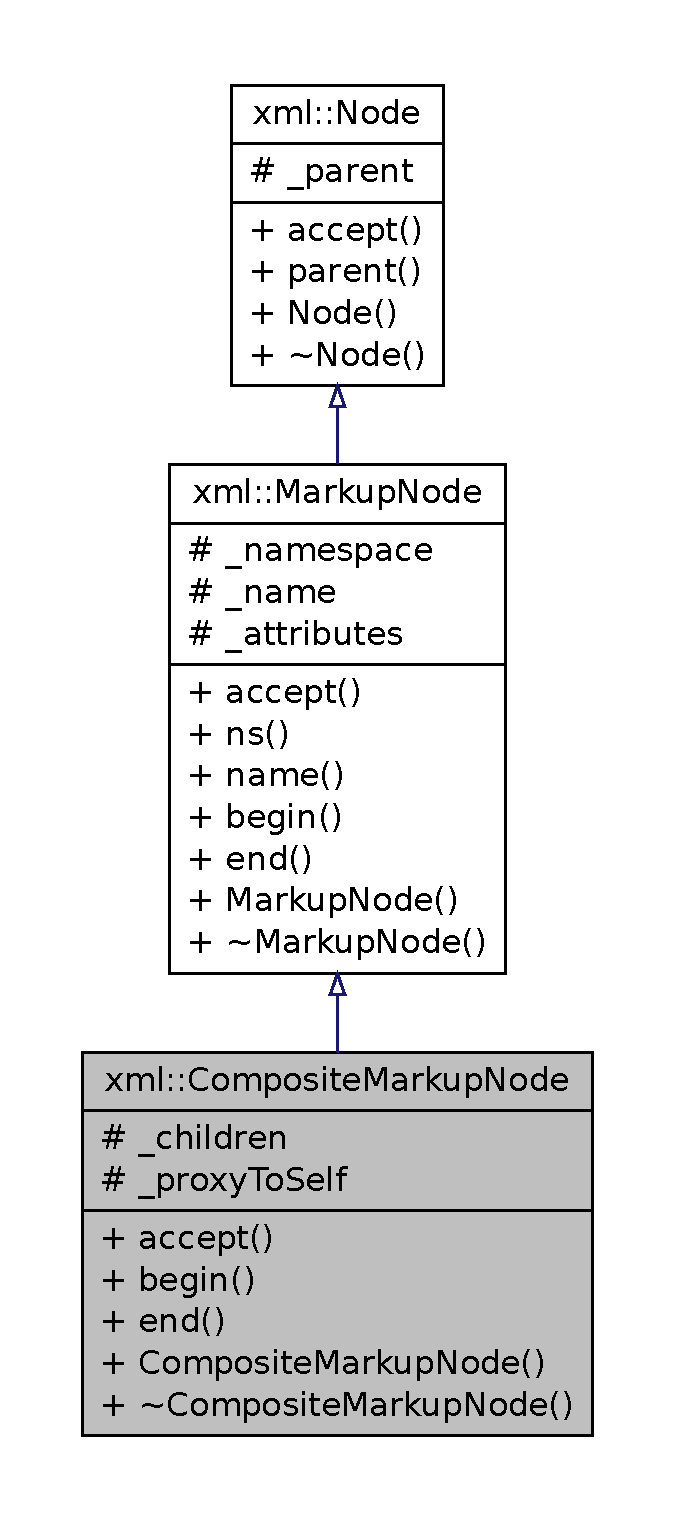
\includegraphics[height=600pt]{classxml_1_1_composite_markup_node__inherit__graph}
\end{center}
\end{figure}


Graphe de collaboration de xml::CompositeMarkupNode:
\nopagebreak
\begin{figure}[H]
\begin{center}
\leavevmode
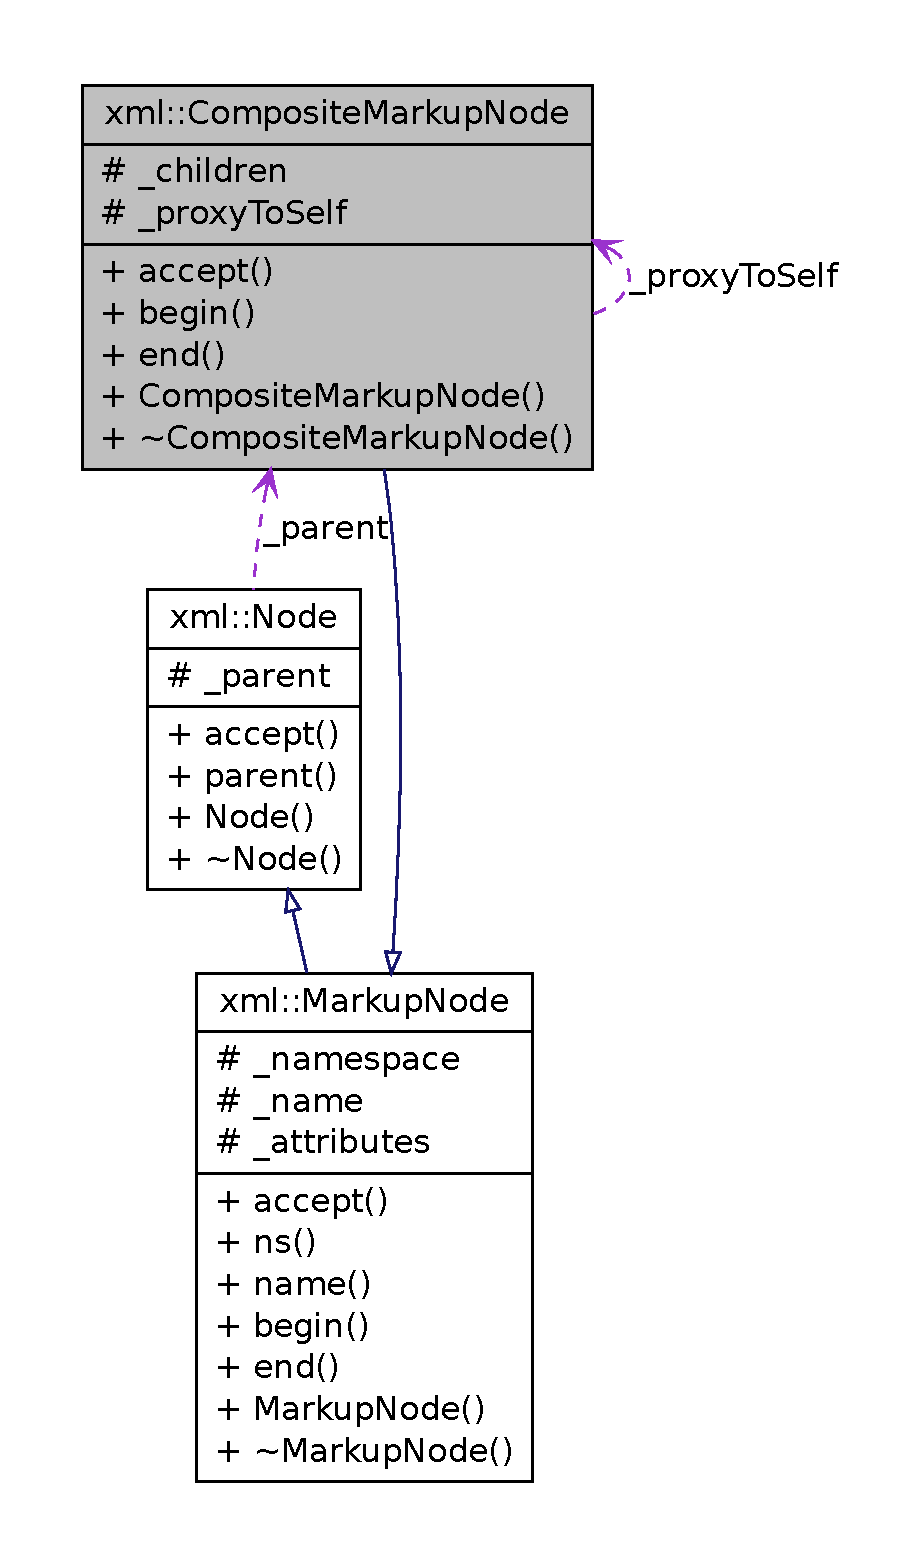
\includegraphics[height=600pt]{classxml_1_1_composite_markup_node__coll__graph}
\end{center}
\end{figure}
\subsection*{Types publics}
\begin{DoxyCompactItemize}
\item 
typedef std::list$<$ \hyperlink{classxml_1_1_node}{Node} $\ast$ $>$ \hyperlink{classxml_1_1_composite_markup_node_ac70e1fdb5fc2e0011378f7284c31fe5c}{Children}
\item 
typedef \_\-Children::const\_\-iterator \hyperlink{classxml_1_1_composite_markup_node_abdd7123eab75fb90a4a95b1976693ed7}{ChildrenIterator}
\end{DoxyCompactItemize}
\subsection*{Fonctions membres publiques}
\begin{DoxyCompactItemize}
\item 
virtual void \hyperlink{classxml_1_1_composite_markup_node_a6c61880592cc2e911517bb3e54c3c987}{accept} (\hyperlink{classxml_1_1_interface_node_visitor}{InterfaceNodeVisitor} \&visitor) const 
\item 
\hyperlink{classxml_1_1_composite_markup_node_abdd7123eab75fb90a4a95b1976693ed7}{ChildrenIterator} \hyperlink{classxml_1_1_composite_markup_node_a124753f641dc4612cee80fd289bf68a6}{begin} () const 
\item 
\hyperlink{classxml_1_1_composite_markup_node_abdd7123eab75fb90a4a95b1976693ed7}{ChildrenIterator} \hyperlink{classxml_1_1_composite_markup_node_aeebeee1fc877fe102bad454d2ffa5bba}{end} () const 
\item 
\hyperlink{classxml_1_1_composite_markup_node_a9f3c506e2b460608f2bc93d5288a7f92}{CompositeMarkupNode} (\hyperlink{classxml_1_1_composite_markup_node}{CompositeMarkupNode} $\ast$$\ast$parent, const std::string \&ns, const std::string \&name, const \hyperlink{classxml_1_1_markup_node_ade6f6045d18042d1a87f80f308f177fb}{Attributes} \&attributes, \hyperlink{classxml_1_1_composite_markup_node}{CompositeMarkupNode} $\ast$\&proxyToSelf, const \hyperlink{classxml_1_1_composite_markup_node_ac70e1fdb5fc2e0011378f7284c31fe5c}{Children} \&children)
\item 
virtual \hyperlink{classxml_1_1_composite_markup_node_a5f8800acf40291ab0cf1b098ae8b82f6}{$\sim$CompositeMarkupNode} ()
\end{DoxyCompactItemize}
\subsection*{Types protégés}
\begin{DoxyCompactItemize}
\item 
typedef std::list$<$ \hyperlink{classxml_1_1_node}{Node} $\ast$ $>$ \hyperlink{classxml_1_1_composite_markup_node_a48287f15a3192f936b0be50e1b2ea13e}{\_\-Children}
\end{DoxyCompactItemize}
\subsection*{Attributs protégés}
\begin{DoxyCompactItemize}
\item 
\hyperlink{classxml_1_1_composite_markup_node_a48287f15a3192f936b0be50e1b2ea13e}{\_\-Children} \hyperlink{classxml_1_1_composite_markup_node_a29a3971e681fe129d60f8ede9d05fb3e}{\_\-children}
\item 
\hyperlink{classxml_1_1_composite_markup_node}{CompositeMarkupNode} $\ast$\& \hyperlink{classxml_1_1_composite_markup_node_a237a9006a0fe8fb8c1b19c323fec4feb}{\_\-proxyToSelf}
\end{DoxyCompactItemize}


\subsection{Description détaillée}


Définition à la ligne 19 du fichier CompositeMarkupNode.hh.



\subsection{Documentation des définitions de type membres}
\hypertarget{classxml_1_1_composite_markup_node_a48287f15a3192f936b0be50e1b2ea13e}{
\index{xml::CompositeMarkupNode@{xml::CompositeMarkupNode}!\_\-Children@{\_\-Children}}
\index{\_\-Children@{\_\-Children}!xml::CompositeMarkupNode@{xml::CompositeMarkupNode}}
\subsubsection[{\_\-Children}]{\setlength{\rightskip}{0pt plus 5cm}typedef std::list$<${\bf Node}$\ast$$>$ {\bf xml::CompositeMarkupNode::\_\-Children}\hspace{0.3cm}{\ttfamily  \mbox{[}protected\mbox{]}}}}
\label{classxml_1_1_composite_markup_node_a48287f15a3192f936b0be50e1b2ea13e}


Définition à la ligne 22 du fichier CompositeMarkupNode.hh.

\hypertarget{classxml_1_1_composite_markup_node_ac70e1fdb5fc2e0011378f7284c31fe5c}{
\index{xml::CompositeMarkupNode@{xml::CompositeMarkupNode}!Children@{Children}}
\index{Children@{Children}!xml::CompositeMarkupNode@{xml::CompositeMarkupNode}}
\subsubsection[{Children}]{\setlength{\rightskip}{0pt plus 5cm}typedef std::list$<${\bf Node}$\ast$$>$ {\bf xml::CompositeMarkupNode::Children}}}
\label{classxml_1_1_composite_markup_node_ac70e1fdb5fc2e0011378f7284c31fe5c}


Définition à la ligne 27 du fichier CompositeMarkupNode.hh.

\hypertarget{classxml_1_1_composite_markup_node_abdd7123eab75fb90a4a95b1976693ed7}{
\index{xml::CompositeMarkupNode@{xml::CompositeMarkupNode}!ChildrenIterator@{ChildrenIterator}}
\index{ChildrenIterator@{ChildrenIterator}!xml::CompositeMarkupNode@{xml::CompositeMarkupNode}}
\subsubsection[{ChildrenIterator}]{\setlength{\rightskip}{0pt plus 5cm}typedef \_\-Children::const\_\-iterator {\bf xml::CompositeMarkupNode::ChildrenIterator}}}
\label{classxml_1_1_composite_markup_node_abdd7123eab75fb90a4a95b1976693ed7}


Définition à la ligne 28 du fichier CompositeMarkupNode.hh.



\subsection{Documentation des constructeurs et destructeur}
\hypertarget{classxml_1_1_composite_markup_node_a9f3c506e2b460608f2bc93d5288a7f92}{
\index{xml::CompositeMarkupNode@{xml::CompositeMarkupNode}!CompositeMarkupNode@{CompositeMarkupNode}}
\index{CompositeMarkupNode@{CompositeMarkupNode}!xml::CompositeMarkupNode@{xml::CompositeMarkupNode}}
\subsubsection[{CompositeMarkupNode}]{\setlength{\rightskip}{0pt plus 5cm}xml::CompositeMarkupNode::CompositeMarkupNode (
\begin{DoxyParamCaption}
\item[{{\bf CompositeMarkupNode} $\ast$$\ast$}]{ parent, }
\item[{const std::string \&}]{ ns, }
\item[{const std::string \&}]{ name, }
\item[{const {\bf Attributes} \&}]{ attributes, }
\item[{{\bf CompositeMarkupNode} $\ast$\&}]{ proxyToSelf, }
\item[{const {\bf Children} \&}]{ children}
\end{DoxyParamCaption}
)}}
\label{classxml_1_1_composite_markup_node_a9f3c506e2b460608f2bc93d5288a7f92}


Définition à la ligne 49 du fichier CompositeMarkupNode.cpp.

\hypertarget{classxml_1_1_composite_markup_node_a5f8800acf40291ab0cf1b098ae8b82f6}{
\index{xml::CompositeMarkupNode@{xml::CompositeMarkupNode}!$\sim$CompositeMarkupNode@{$\sim$CompositeMarkupNode}}
\index{$\sim$CompositeMarkupNode@{$\sim$CompositeMarkupNode}!xml::CompositeMarkupNode@{xml::CompositeMarkupNode}}
\subsubsection[{$\sim$CompositeMarkupNode}]{\setlength{\rightskip}{0pt plus 5cm}xml::CompositeMarkupNode::$\sim$CompositeMarkupNode (
\begin{DoxyParamCaption}
{}
\end{DoxyParamCaption}
)\hspace{0.3cm}{\ttfamily  \mbox{[}virtual\mbox{]}}}}
\label{classxml_1_1_composite_markup_node_a5f8800acf40291ab0cf1b098ae8b82f6}


Définition à la ligne 60 du fichier CompositeMarkupNode.cpp.



\subsection{Documentation des fonctions membres}
\hypertarget{classxml_1_1_composite_markup_node_a6c61880592cc2e911517bb3e54c3c987}{
\index{xml::CompositeMarkupNode@{xml::CompositeMarkupNode}!accept@{accept}}
\index{accept@{accept}!xml::CompositeMarkupNode@{xml::CompositeMarkupNode}}
\subsubsection[{accept}]{\setlength{\rightskip}{0pt plus 5cm}void xml::CompositeMarkupNode::accept (
\begin{DoxyParamCaption}
\item[{{\bf InterfaceNodeVisitor} \&}]{ visitor}
\end{DoxyParamCaption}
) const\hspace{0.3cm}{\ttfamily  \mbox{[}virtual\mbox{]}}}}
\label{classxml_1_1_composite_markup_node_a6c61880592cc2e911517bb3e54c3c987}


Réimplémentée à partir de \hyperlink{classxml_1_1_markup_node_ae70b538ce71b427c1ea552b0b41c3b34}{xml::MarkupNode}.



Définition à la ligne 30 du fichier CompositeMarkupNode.cpp.



Voici le graphe d'appel pour cette fonction :
\nopagebreak
\begin{figure}[H]
\begin{center}
\leavevmode
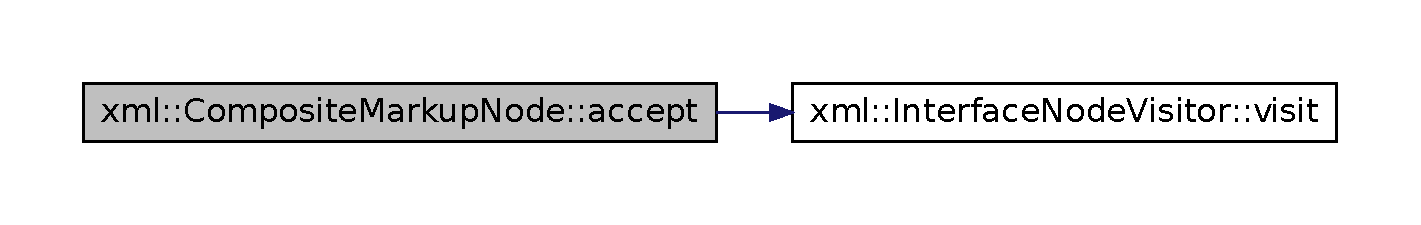
\includegraphics[width=400pt]{classxml_1_1_composite_markup_node_a6c61880592cc2e911517bb3e54c3c987_cgraph}
\end{center}
\end{figure}


\hypertarget{classxml_1_1_composite_markup_node_a124753f641dc4612cee80fd289bf68a6}{
\index{xml::CompositeMarkupNode@{xml::CompositeMarkupNode}!begin@{begin}}
\index{begin@{begin}!xml::CompositeMarkupNode@{xml::CompositeMarkupNode}}
\subsubsection[{begin}]{\setlength{\rightskip}{0pt plus 5cm}{\bf CompositeMarkupNode::ChildrenIterator} xml::CompositeMarkupNode::begin (
\begin{DoxyParamCaption}
{}
\end{DoxyParamCaption}
) const}}
\label{classxml_1_1_composite_markup_node_a124753f641dc4612cee80fd289bf68a6}


Réimplémentée à partir de \hyperlink{classxml_1_1_markup_node_a48aac1f80b326393fdac05835604c69f}{xml::MarkupNode}.



Définition à la ligne 35 du fichier CompositeMarkupNode.cpp.

\hypertarget{classxml_1_1_composite_markup_node_aeebeee1fc877fe102bad454d2ffa5bba}{
\index{xml::CompositeMarkupNode@{xml::CompositeMarkupNode}!end@{end}}
\index{end@{end}!xml::CompositeMarkupNode@{xml::CompositeMarkupNode}}
\subsubsection[{end}]{\setlength{\rightskip}{0pt plus 5cm}{\bf CompositeMarkupNode::ChildrenIterator} xml::CompositeMarkupNode::end (
\begin{DoxyParamCaption}
{}
\end{DoxyParamCaption}
) const}}
\label{classxml_1_1_composite_markup_node_aeebeee1fc877fe102bad454d2ffa5bba}


Réimplémentée à partir de \hyperlink{classxml_1_1_markup_node_a3b63a8ea94999e2f688f6dc606f3e24b}{xml::MarkupNode}.



Définition à la ligne 40 du fichier CompositeMarkupNode.cpp.



\subsection{Documentation des données membres}
\hypertarget{classxml_1_1_composite_markup_node_a29a3971e681fe129d60f8ede9d05fb3e}{
\index{xml::CompositeMarkupNode@{xml::CompositeMarkupNode}!\_\-children@{\_\-children}}
\index{\_\-children@{\_\-children}!xml::CompositeMarkupNode@{xml::CompositeMarkupNode}}
\subsubsection[{\_\-children}]{\setlength{\rightskip}{0pt plus 5cm}{\bf \_\-Children} {\bf xml::CompositeMarkupNode::\_\-children}\hspace{0.3cm}{\ttfamily  \mbox{[}protected\mbox{]}}}}
\label{classxml_1_1_composite_markup_node_a29a3971e681fe129d60f8ede9d05fb3e}


Définition à la ligne 93 du fichier CompositeMarkupNode.hh.

\hypertarget{classxml_1_1_composite_markup_node_a237a9006a0fe8fb8c1b19c323fec4feb}{
\index{xml::CompositeMarkupNode@{xml::CompositeMarkupNode}!\_\-proxyToSelf@{\_\-proxyToSelf}}
\index{\_\-proxyToSelf@{\_\-proxyToSelf}!xml::CompositeMarkupNode@{xml::CompositeMarkupNode}}
\subsubsection[{\_\-proxyToSelf}]{\setlength{\rightskip}{0pt plus 5cm}{\bf CompositeMarkupNode}$\ast$\& {\bf xml::CompositeMarkupNode::\_\-proxyToSelf}\hspace{0.3cm}{\ttfamily  \mbox{[}protected\mbox{]}}}}
\label{classxml_1_1_composite_markup_node_a237a9006a0fe8fb8c1b19c323fec4feb}


Définition à la ligne 95 du fichier CompositeMarkupNode.hh.



La documentation de cette classe a été générée à partir des fichiers suivants :\begin{DoxyCompactItemize}
\item 
src/\hyperlink{_composite_markup_node_8hh}{CompositeMarkupNode.hh}\item 
src/\hyperlink{_composite_markup_node_8cpp}{CompositeMarkupNode.cpp}\end{DoxyCompactItemize}

\hypertarget{classxml_1_1_dot_output_visitor}{
\section{Référence de la classe xml::DotOutputVisitor}
\label{classxml_1_1_dot_output_visitor}\index{xml::DotOutputVisitor@{xml::DotOutputVisitor}}
}


{\ttfamily \#include $<$DotOutputVisitor.hh$>$}



Graphe d'héritage de xml::DotOutputVisitor:
\nopagebreak
\begin{figure}[H]
\begin{center}
\leavevmode
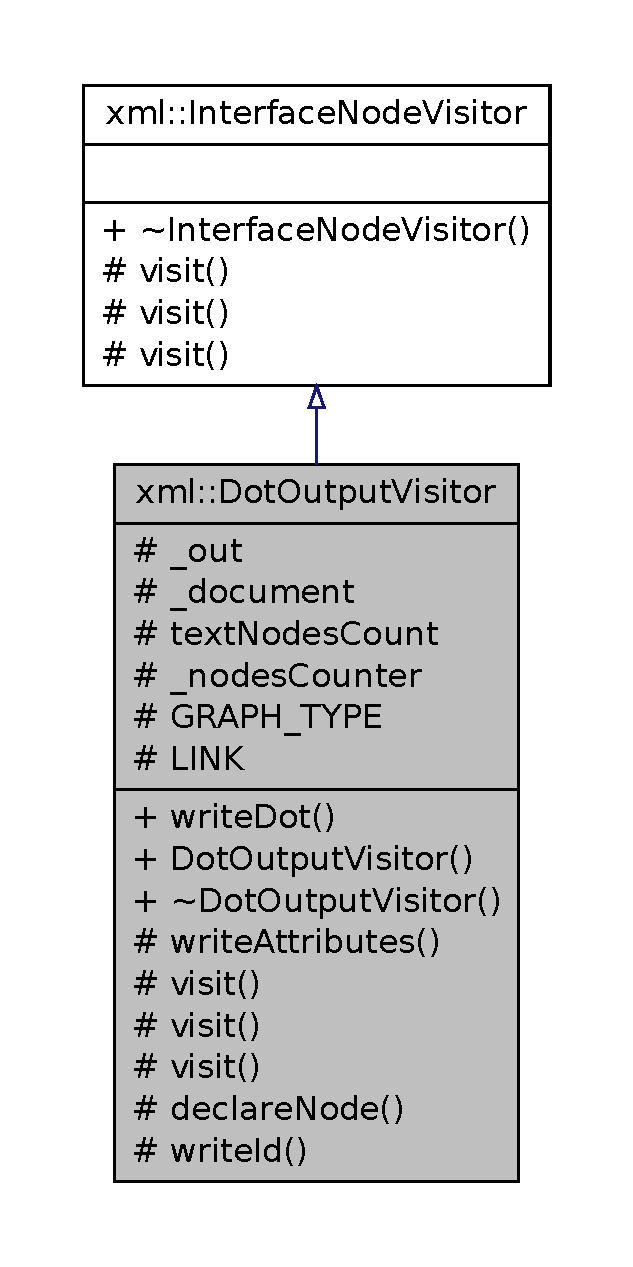
\includegraphics[height=600pt]{classxml_1_1_dot_output_visitor__inherit__graph}
\end{center}
\end{figure}


Graphe de collaboration de xml::DotOutputVisitor:
\nopagebreak
\begin{figure}[H]
\begin{center}
\leavevmode
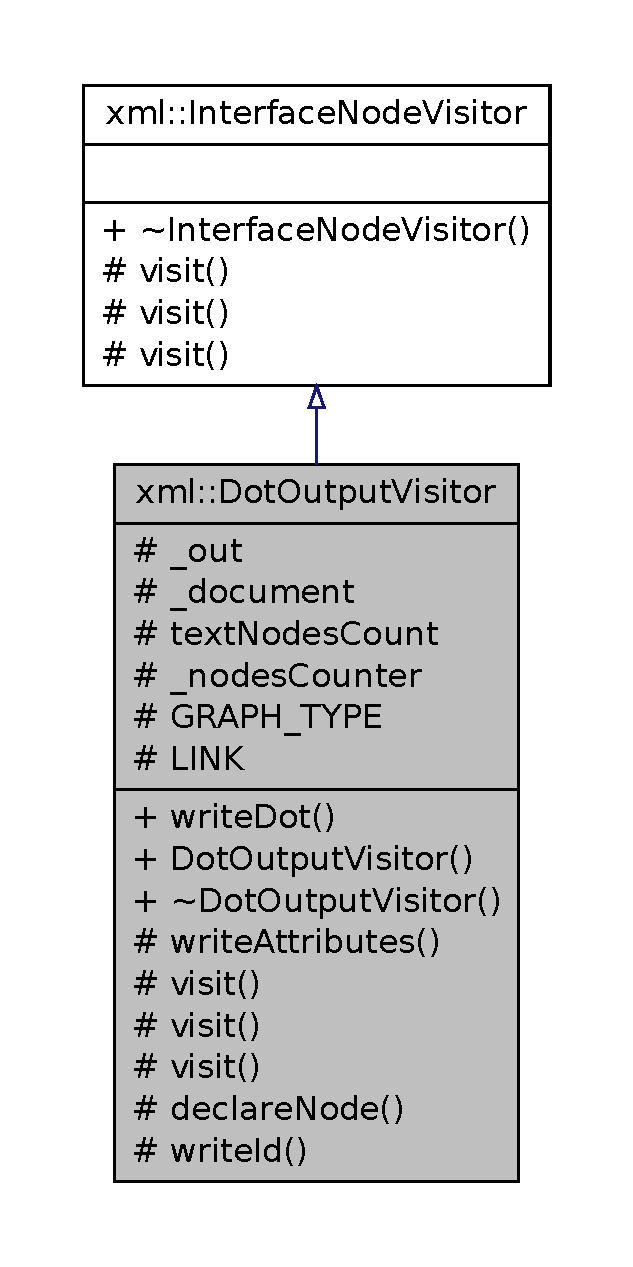
\includegraphics[height=600pt]{classxml_1_1_dot_output_visitor__coll__graph}
\end{center}
\end{figure}
\subsection*{Fonctions membres publiques}
\begin{DoxyCompactItemize}
\item 
void \hyperlink{classxml_1_1_dot_output_visitor_a329cc7e31f291ccbebf5029325321ee0}{writeDot} (\hyperlink{classxml_1_1_node}{Node} $\ast$node)
\item 
\hyperlink{classxml_1_1_dot_output_visitor_a572e83719b4820a194c8094fd283caea}{DotOutputVisitor} (std::ostream \&out, std::string graphName)
\item 
virtual \hyperlink{classxml_1_1_dot_output_visitor_a58f12e15968fb6d1d66853b8106212fe}{$\sim$DotOutputVisitor} ()
\end{DoxyCompactItemize}
\subsection*{Fonctions membres protégées}
\begin{DoxyCompactItemize}
\item 
void \hyperlink{classxml_1_1_dot_output_visitor_a8c9f18ff770920e75f040dff46570f0c}{writeAttributes} (const \hyperlink{classxml_1_1_markup_node}{MarkupNode} \&node)
\item 
virtual void \hyperlink{classxml_1_1_dot_output_visitor_ad18c9818c42e6d0f515fa583d1a01ec8}{visit} (const \hyperlink{classxml_1_1_text_node}{TextNode} \&node)
\item 
virtual void \hyperlink{classxml_1_1_dot_output_visitor_a2744dca685af0e8a420624c48f7eea53}{visit} (const \hyperlink{classxml_1_1_markup_node}{MarkupNode} \&node)
\item 
virtual void \hyperlink{classxml_1_1_dot_output_visitor_a1755fb782d2d50ab28dc41045e60c69b}{visit} (const \hyperlink{classxml_1_1_composite_markup_node}{CompositeMarkupNode} \&node)
\item 
void \hyperlink{classxml_1_1_dot_output_visitor_abc55a0a0143a2ec38adb43ceacc5c244}{declareNode} (const \hyperlink{classxml_1_1_node}{Node} \&node, std::string label)
\item 
void \hyperlink{classxml_1_1_dot_output_visitor_a4df18e8a595e20fd1a7d6f48fe7865fb}{writeId} (const \hyperlink{classxml_1_1_node}{Node} \&node)
\end{DoxyCompactItemize}
\subsection*{Attributs protégés}
\begin{DoxyCompactItemize}
\item 
std::ostream \& \hyperlink{classxml_1_1_dot_output_visitor_a5bd82f9f1db24368e579e075a1929ca6}{\_\-out}
\item 
std::string \hyperlink{classxml_1_1_dot_output_visitor_a7ff9e32ea1c710644289ef6f8479f872}{\_\-document}
\item 
int \hyperlink{classxml_1_1_dot_output_visitor_a65f377e3a153b5cec4ba84a3c70c8d29}{textNodesCount}
\item 
int \hyperlink{classxml_1_1_dot_output_visitor_a250aac727f10406e22c019cc262f3327}{\_\-nodesCounter}
\end{DoxyCompactItemize}
\subsection*{Attributs protégés statiques}
\begin{DoxyCompactItemize}
\item 
static const std::string \hyperlink{classxml_1_1_dot_output_visitor_a5cf6c70f78fa4edced8f89d18b95c0d0}{GRAPH\_\-TYPE} = \char`\"{}digraph\char`\"{}
\item 
static const std::string \hyperlink{classxml_1_1_dot_output_visitor_a0df19df5cbdc9101aad2e71d2e87c33c}{LINK} = \char`\"{} -\/$>$ \char`\"{}
\end{DoxyCompactItemize}


\subsection{Description détaillée}


Définition à la ligne 24 du fichier DotOutputVisitor.hh.



\subsection{Documentation des constructeurs et destructeur}
\hypertarget{classxml_1_1_dot_output_visitor_a572e83719b4820a194c8094fd283caea}{
\index{xml::DotOutputVisitor@{xml::DotOutputVisitor}!DotOutputVisitor@{DotOutputVisitor}}
\index{DotOutputVisitor@{DotOutputVisitor}!xml::DotOutputVisitor@{xml::DotOutputVisitor}}
\subsubsection[{DotOutputVisitor}]{\setlength{\rightskip}{0pt plus 5cm}xml::DotOutputVisitor::DotOutputVisitor (
\begin{DoxyParamCaption}
\item[{std::ostream \&}]{ out, }
\item[{std::string}]{ graphName}
\end{DoxyParamCaption}
)}}
\label{classxml_1_1_dot_output_visitor_a572e83719b4820a194c8094fd283caea}
\hypertarget{classxml_1_1_dot_output_visitor_a58f12e15968fb6d1d66853b8106212fe}{
\index{xml::DotOutputVisitor@{xml::DotOutputVisitor}!$\sim$DotOutputVisitor@{$\sim$DotOutputVisitor}}
\index{$\sim$DotOutputVisitor@{$\sim$DotOutputVisitor}!xml::DotOutputVisitor@{xml::DotOutputVisitor}}
\subsubsection[{$\sim$DotOutputVisitor}]{\setlength{\rightskip}{0pt plus 5cm}xml::DotOutputVisitor::$\sim$DotOutputVisitor (
\begin{DoxyParamCaption}
{}
\end{DoxyParamCaption}
)\hspace{0.3cm}{\ttfamily  \mbox{[}virtual\mbox{]}}}}
\label{classxml_1_1_dot_output_visitor_a58f12e15968fb6d1d66853b8106212fe}


Définition à la ligne 49 du fichier DotOutputVisitor.cpp.



\subsection{Documentation des fonctions membres}
\hypertarget{classxml_1_1_dot_output_visitor_abc55a0a0143a2ec38adb43ceacc5c244}{
\index{xml::DotOutputVisitor@{xml::DotOutputVisitor}!declareNode@{declareNode}}
\index{declareNode@{declareNode}!xml::DotOutputVisitor@{xml::DotOutputVisitor}}
\subsubsection[{declareNode}]{\setlength{\rightskip}{0pt plus 5cm}void xml::DotOutputVisitor::declareNode (
\begin{DoxyParamCaption}
\item[{const {\bf Node} \&}]{ node, }
\item[{std::string}]{ label}
\end{DoxyParamCaption}
)\hspace{0.3cm}{\ttfamily  \mbox{[}protected\mbox{]}}}}
\label{classxml_1_1_dot_output_visitor_abc55a0a0143a2ec38adb43ceacc5c244}
\hypertarget{classxml_1_1_dot_output_visitor_a2744dca685af0e8a420624c48f7eea53}{
\index{xml::DotOutputVisitor@{xml::DotOutputVisitor}!visit@{visit}}
\index{visit@{visit}!xml::DotOutputVisitor@{xml::DotOutputVisitor}}
\subsubsection[{visit}]{\setlength{\rightskip}{0pt plus 5cm}void xml::DotOutputVisitor::visit (
\begin{DoxyParamCaption}
\item[{const {\bf MarkupNode} \&}]{ node}
\end{DoxyParamCaption}
)\hspace{0.3cm}{\ttfamily  \mbox{[}protected, virtual\mbox{]}}}}
\label{classxml_1_1_dot_output_visitor_a2744dca685af0e8a420624c48f7eea53}


Implémente \hyperlink{classxml_1_1_interface_node_visitor_a53b33aabb8a79d4b1715c7664671d326}{xml::InterfaceNodeVisitor}.



Définition à la ligne 85 du fichier DotOutputVisitor.cpp.

\hypertarget{classxml_1_1_dot_output_visitor_a1755fb782d2d50ab28dc41045e60c69b}{
\index{xml::DotOutputVisitor@{xml::DotOutputVisitor}!visit@{visit}}
\index{visit@{visit}!xml::DotOutputVisitor@{xml::DotOutputVisitor}}
\subsubsection[{visit}]{\setlength{\rightskip}{0pt plus 5cm}void xml::DotOutputVisitor::visit (
\begin{DoxyParamCaption}
\item[{const {\bf CompositeMarkupNode} \&}]{ node}
\end{DoxyParamCaption}
)\hspace{0.3cm}{\ttfamily  \mbox{[}protected, virtual\mbox{]}}}}
\label{classxml_1_1_dot_output_visitor_a1755fb782d2d50ab28dc41045e60c69b}


Implémente \hyperlink{classxml_1_1_interface_node_visitor_afd6306ffd03380f21f436234b314c34d}{xml::InterfaceNodeVisitor}.



Définition à la ligne 92 du fichier DotOutputVisitor.cpp.

\hypertarget{classxml_1_1_dot_output_visitor_ad18c9818c42e6d0f515fa583d1a01ec8}{
\index{xml::DotOutputVisitor@{xml::DotOutputVisitor}!visit@{visit}}
\index{visit@{visit}!xml::DotOutputVisitor@{xml::DotOutputVisitor}}
\subsubsection[{visit}]{\setlength{\rightskip}{0pt plus 5cm}void xml::DotOutputVisitor::visit (
\begin{DoxyParamCaption}
\item[{const {\bf TextNode} \&}]{ node}
\end{DoxyParamCaption}
)\hspace{0.3cm}{\ttfamily  \mbox{[}protected, virtual\mbox{]}}}}
\label{classxml_1_1_dot_output_visitor_ad18c9818c42e6d0f515fa583d1a01ec8}


Implémente \hyperlink{classxml_1_1_interface_node_visitor_a22a8a333e5cf2da1f1ac9f8f1f376a89}{xml::InterfaceNodeVisitor}.



Définition à la ligne 77 du fichier DotOutputVisitor.cpp.

\hypertarget{classxml_1_1_dot_output_visitor_a8c9f18ff770920e75f040dff46570f0c}{
\index{xml::DotOutputVisitor@{xml::DotOutputVisitor}!writeAttributes@{writeAttributes}}
\index{writeAttributes@{writeAttributes}!xml::DotOutputVisitor@{xml::DotOutputVisitor}}
\subsubsection[{writeAttributes}]{\setlength{\rightskip}{0pt plus 5cm}void xml::DotOutputVisitor::writeAttributes (
\begin{DoxyParamCaption}
\item[{const {\bf MarkupNode} \&}]{ node}
\end{DoxyParamCaption}
)\hspace{0.3cm}{\ttfamily  \mbox{[}protected\mbox{]}}}}
\label{classxml_1_1_dot_output_visitor_a8c9f18ff770920e75f040dff46570f0c}


Définition à la ligne 59 du fichier DotOutputVisitor.cpp.

\hypertarget{classxml_1_1_dot_output_visitor_a329cc7e31f291ccbebf5029325321ee0}{
\index{xml::DotOutputVisitor@{xml::DotOutputVisitor}!writeDot@{writeDot}}
\index{writeDot@{writeDot}!xml::DotOutputVisitor@{xml::DotOutputVisitor}}
\subsubsection[{writeDot}]{\setlength{\rightskip}{0pt plus 5cm}void xml::DotOutputVisitor::writeDot (
\begin{DoxyParamCaption}
\item[{{\bf Node} $\ast$}]{ node}
\end{DoxyParamCaption}
)}}
\label{classxml_1_1_dot_output_visitor_a329cc7e31f291ccbebf5029325321ee0}


Définition à la ligne 69 du fichier DotOutputVisitor.cpp.

\hypertarget{classxml_1_1_dot_output_visitor_a4df18e8a595e20fd1a7d6f48fe7865fb}{
\index{xml::DotOutputVisitor@{xml::DotOutputVisitor}!writeId@{writeId}}
\index{writeId@{writeId}!xml::DotOutputVisitor@{xml::DotOutputVisitor}}
\subsubsection[{writeId}]{\setlength{\rightskip}{0pt plus 5cm}void xml::DotOutputVisitor::writeId (
\begin{DoxyParamCaption}
\item[{const {\bf Node} \&}]{ node}
\end{DoxyParamCaption}
)\hspace{0.3cm}{\ttfamily  \mbox{[}protected\mbox{]}}}}
\label{classxml_1_1_dot_output_visitor_a4df18e8a595e20fd1a7d6f48fe7865fb}


Définition à la ligne 114 du fichier DotOutputVisitor.cpp.



\subsection{Documentation des données membres}
\hypertarget{classxml_1_1_dot_output_visitor_a7ff9e32ea1c710644289ef6f8479f872}{
\index{xml::DotOutputVisitor@{xml::DotOutputVisitor}!\_\-document@{\_\-document}}
\index{\_\-document@{\_\-document}!xml::DotOutputVisitor@{xml::DotOutputVisitor}}
\subsubsection[{\_\-document}]{\setlength{\rightskip}{0pt plus 5cm}std::string {\bf xml::DotOutputVisitor::\_\-document}\hspace{0.3cm}{\ttfamily  \mbox{[}protected\mbox{]}}}}
\label{classxml_1_1_dot_output_visitor_a7ff9e32ea1c710644289ef6f8479f872}


Définition à la ligne 62 du fichier DotOutputVisitor.hh.

\hypertarget{classxml_1_1_dot_output_visitor_a250aac727f10406e22c019cc262f3327}{
\index{xml::DotOutputVisitor@{xml::DotOutputVisitor}!\_\-nodesCounter@{\_\-nodesCounter}}
\index{\_\-nodesCounter@{\_\-nodesCounter}!xml::DotOutputVisitor@{xml::DotOutputVisitor}}
\subsubsection[{\_\-nodesCounter}]{\setlength{\rightskip}{0pt plus 5cm}int {\bf xml::DotOutputVisitor::\_\-nodesCounter}\hspace{0.3cm}{\ttfamily  \mbox{[}protected\mbox{]}}}}
\label{classxml_1_1_dot_output_visitor_a250aac727f10406e22c019cc262f3327}


Définition à la ligne 64 du fichier DotOutputVisitor.hh.

\hypertarget{classxml_1_1_dot_output_visitor_a5bd82f9f1db24368e579e075a1929ca6}{
\index{xml::DotOutputVisitor@{xml::DotOutputVisitor}!\_\-out@{\_\-out}}
\index{\_\-out@{\_\-out}!xml::DotOutputVisitor@{xml::DotOutputVisitor}}
\subsubsection[{\_\-out}]{\setlength{\rightskip}{0pt plus 5cm}std::ostream\& {\bf xml::DotOutputVisitor::\_\-out}\hspace{0.3cm}{\ttfamily  \mbox{[}protected\mbox{]}}}}
\label{classxml_1_1_dot_output_visitor_a5bd82f9f1db24368e579e075a1929ca6}


Définition à la ligne 61 du fichier DotOutputVisitor.hh.

\hypertarget{classxml_1_1_dot_output_visitor_a5cf6c70f78fa4edced8f89d18b95c0d0}{
\index{xml::DotOutputVisitor@{xml::DotOutputVisitor}!GRAPH\_\-TYPE@{GRAPH\_\-TYPE}}
\index{GRAPH\_\-TYPE@{GRAPH\_\-TYPE}!xml::DotOutputVisitor@{xml::DotOutputVisitor}}
\subsubsection[{GRAPH\_\-TYPE}]{\setlength{\rightskip}{0pt plus 5cm}const std::string {\bf xml::DotOutputVisitor::GRAPH\_\-TYPE} = \char`\"{}digraph\char`\"{}\hspace{0.3cm}{\ttfamily  \mbox{[}static, protected\mbox{]}}}}
\label{classxml_1_1_dot_output_visitor_a5cf6c70f78fa4edced8f89d18b95c0d0}


Définition à la ligne 58 du fichier DotOutputVisitor.hh.

\hypertarget{classxml_1_1_dot_output_visitor_a0df19df5cbdc9101aad2e71d2e87c33c}{
\index{xml::DotOutputVisitor@{xml::DotOutputVisitor}!LINK@{LINK}}
\index{LINK@{LINK}!xml::DotOutputVisitor@{xml::DotOutputVisitor}}
\subsubsection[{LINK}]{\setlength{\rightskip}{0pt plus 5cm}const std::string {\bf xml::DotOutputVisitor::LINK} = \char`\"{} -\/$>$ \char`\"{}\hspace{0.3cm}{\ttfamily  \mbox{[}static, protected\mbox{]}}}}
\label{classxml_1_1_dot_output_visitor_a0df19df5cbdc9101aad2e71d2e87c33c}


Définition à la ligne 59 du fichier DotOutputVisitor.hh.

\hypertarget{classxml_1_1_dot_output_visitor_a65f377e3a153b5cec4ba84a3c70c8d29}{
\index{xml::DotOutputVisitor@{xml::DotOutputVisitor}!textNodesCount@{textNodesCount}}
\index{textNodesCount@{textNodesCount}!xml::DotOutputVisitor@{xml::DotOutputVisitor}}
\subsubsection[{textNodesCount}]{\setlength{\rightskip}{0pt plus 5cm}int {\bf xml::DotOutputVisitor::textNodesCount}\hspace{0.3cm}{\ttfamily  \mbox{[}protected\mbox{]}}}}
\label{classxml_1_1_dot_output_visitor_a65f377e3a153b5cec4ba84a3c70c8d29}


Définition à la ligne 63 du fichier DotOutputVisitor.hh.



La documentation de cette classe a été générée à partir des fichiers suivants :\begin{DoxyCompactItemize}
\item 
src/\hyperlink{_dot_output_visitor_8hh}{DotOutputVisitor.hh}\item 
src/\hyperlink{_dot_output_visitor_8cpp}{DotOutputVisitor.cpp}\end{DoxyCompactItemize}

\hypertarget{classxml_1_1_interface_node_visitor}{
\section{Référence de la classe xml::InterfaceNodeVisitor}
\label{classxml_1_1_interface_node_visitor}\index{xml::InterfaceNodeVisitor@{xml::InterfaceNodeVisitor}}
}


{\ttfamily \#include $<$InterfaceNodeVisitor.hpp$>$}



Graphe d'héritage de xml::InterfaceNodeVisitor:
\nopagebreak
\begin{figure}[H]
\begin{center}
\leavevmode
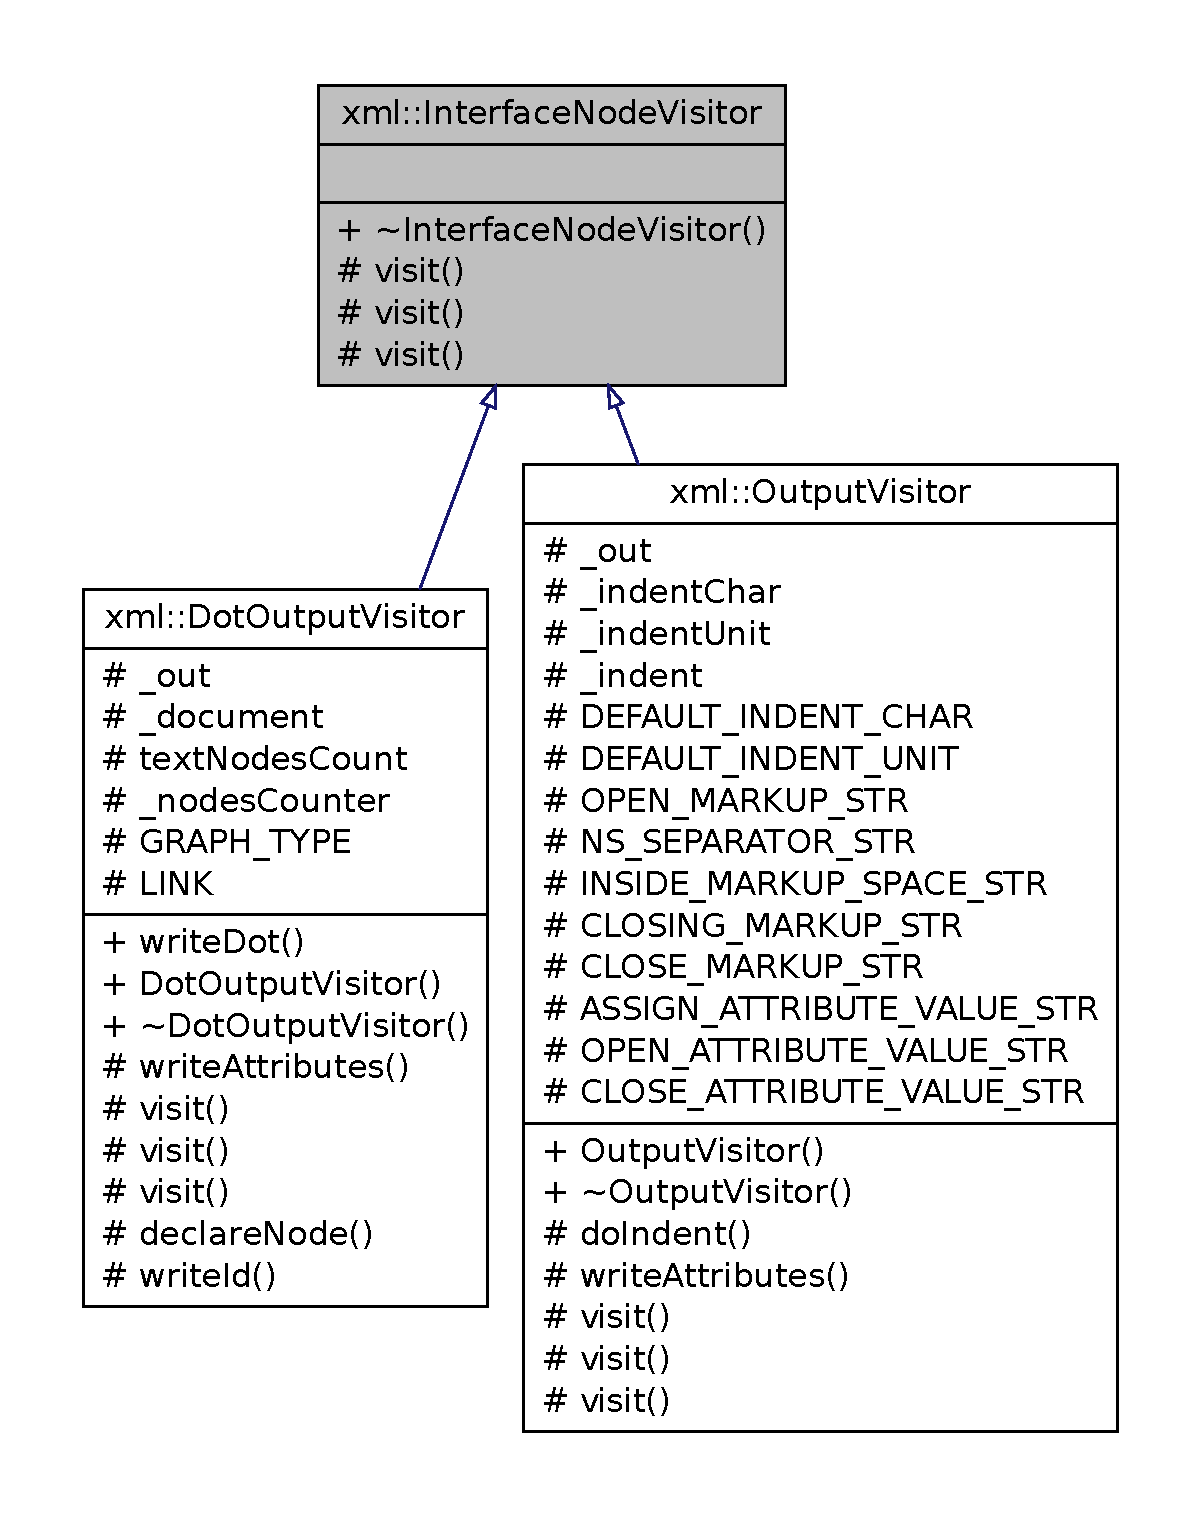
\includegraphics[width=400pt]{classxml_1_1_interface_node_visitor__inherit__graph}
\end{center}
\end{figure}
\subsection*{Fonctions membres publiques}
\begin{DoxyCompactItemize}
\item 
virtual \hyperlink{classxml_1_1_interface_node_visitor_a53c5fa9a736af1450bbc3d95feffe94a}{$\sim$InterfaceNodeVisitor} ()
\end{DoxyCompactItemize}
\subsection*{Fonctions membres protégées}
\begin{DoxyCompactItemize}
\item 
virtual void \hyperlink{classxml_1_1_interface_node_visitor_a22a8a333e5cf2da1f1ac9f8f1f376a89}{visit} (const \hyperlink{classxml_1_1_text_node}{TextNode} \&node)=0
\item 
virtual void \hyperlink{classxml_1_1_interface_node_visitor_a53b33aabb8a79d4b1715c7664671d326}{visit} (const \hyperlink{classxml_1_1_markup_node}{MarkupNode} \&node)=0
\item 
virtual void \hyperlink{classxml_1_1_interface_node_visitor_afd6306ffd03380f21f436234b314c34d}{visit} (const \hyperlink{classxml_1_1_composite_markup_node}{CompositeMarkupNode} \&node)=0
\end{DoxyCompactItemize}
\subsection*{Amis}
\begin{DoxyCompactItemize}
\item 
class \hyperlink{classxml_1_1_interface_node_visitor_abd4faab11b504920cd6f8af02104143c}{TextNode}
\item 
class \hyperlink{classxml_1_1_interface_node_visitor_ac2a462e7a005c065f6778ccc0be88931}{MarkupNode}
\item 
class \hyperlink{classxml_1_1_interface_node_visitor_a8478dddac071858d6a22088eb161a690}{CompositeMarkupNode}
\end{DoxyCompactItemize}


\subsection{Description détaillée}


Définition à la ligne 19 du fichier InterfaceNodeVisitor.hpp.



\subsection{Documentation des constructeurs et destructeur}
\hypertarget{classxml_1_1_interface_node_visitor_a53c5fa9a736af1450bbc3d95feffe94a}{
\index{xml::InterfaceNodeVisitor@{xml::InterfaceNodeVisitor}!$\sim$InterfaceNodeVisitor@{$\sim$InterfaceNodeVisitor}}
\index{$\sim$InterfaceNodeVisitor@{$\sim$InterfaceNodeVisitor}!xml::InterfaceNodeVisitor@{xml::InterfaceNodeVisitor}}
\subsubsection[{$\sim$InterfaceNodeVisitor}]{\setlength{\rightskip}{0pt plus 5cm}virtual xml::InterfaceNodeVisitor::$\sim$InterfaceNodeVisitor (
\begin{DoxyParamCaption}
{}
\end{DoxyParamCaption}
)\hspace{0.3cm}{\ttfamily  \mbox{[}inline, virtual\mbox{]}}}}
\label{classxml_1_1_interface_node_visitor_a53c5fa9a736af1450bbc3d95feffe94a}


Définition à la ligne 22 du fichier InterfaceNodeVisitor.hpp.



\subsection{Documentation des fonctions membres}
\hypertarget{classxml_1_1_interface_node_visitor_a22a8a333e5cf2da1f1ac9f8f1f376a89}{
\index{xml::InterfaceNodeVisitor@{xml::InterfaceNodeVisitor}!visit@{visit}}
\index{visit@{visit}!xml::InterfaceNodeVisitor@{xml::InterfaceNodeVisitor}}
\subsubsection[{visit}]{\setlength{\rightskip}{0pt plus 5cm}virtual void xml::InterfaceNodeVisitor::visit (
\begin{DoxyParamCaption}
\item[{const {\bf TextNode} \&}]{ node}
\end{DoxyParamCaption}
)\hspace{0.3cm}{\ttfamily  \mbox{[}protected, pure virtual\mbox{]}}}}
\label{classxml_1_1_interface_node_visitor_a22a8a333e5cf2da1f1ac9f8f1f376a89}


Implémenté dans \hyperlink{classxml_1_1_dot_output_visitor_ad18c9818c42e6d0f515fa583d1a01ec8}{xml::DotOutputVisitor}, et \hyperlink{classxml_1_1_output_visitor_a33e53f866b31a155bbf29ffda852aaf7}{xml::OutputVisitor}.



Voici le graphe d'appel pour cette fonction :\nopagebreak
\begin{figure}[H]
\begin{center}
\leavevmode
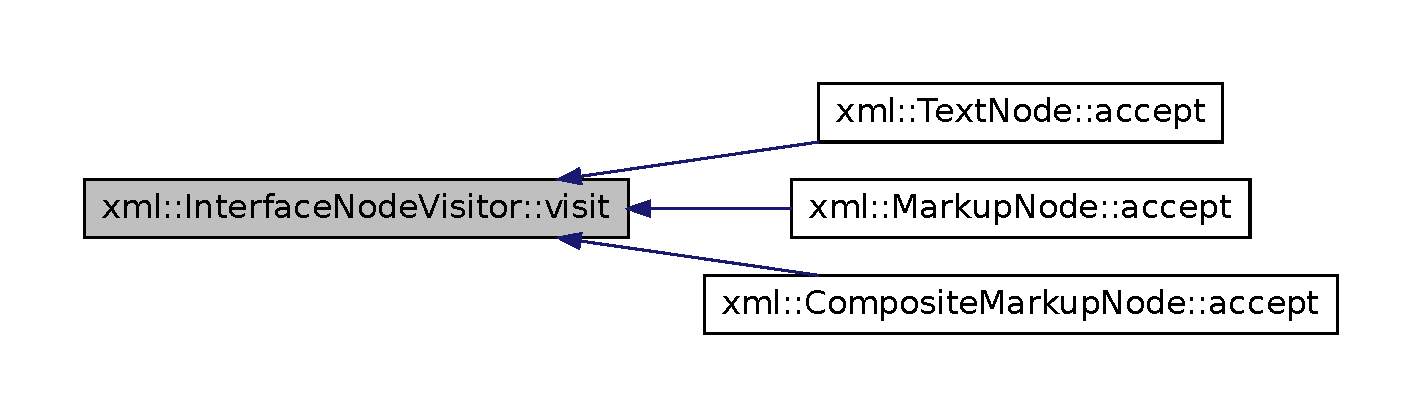
\includegraphics[width=400pt]{classxml_1_1_interface_node_visitor_a22a8a333e5cf2da1f1ac9f8f1f376a89_icgraph}
\end{center}
\end{figure}


\hypertarget{classxml_1_1_interface_node_visitor_afd6306ffd03380f21f436234b314c34d}{
\index{xml::InterfaceNodeVisitor@{xml::InterfaceNodeVisitor}!visit@{visit}}
\index{visit@{visit}!xml::InterfaceNodeVisitor@{xml::InterfaceNodeVisitor}}
\subsubsection[{visit}]{\setlength{\rightskip}{0pt plus 5cm}virtual void xml::InterfaceNodeVisitor::visit (
\begin{DoxyParamCaption}
\item[{const {\bf CompositeMarkupNode} \&}]{ node}
\end{DoxyParamCaption}
)\hspace{0.3cm}{\ttfamily  \mbox{[}protected, pure virtual\mbox{]}}}}
\label{classxml_1_1_interface_node_visitor_afd6306ffd03380f21f436234b314c34d}


Implémenté dans \hyperlink{classxml_1_1_dot_output_visitor_a1755fb782d2d50ab28dc41045e60c69b}{xml::DotOutputVisitor}, et \hyperlink{classxml_1_1_output_visitor_addfc73ae3643a8285b5f892eff1a6066}{xml::OutputVisitor}.

\hypertarget{classxml_1_1_interface_node_visitor_a53b33aabb8a79d4b1715c7664671d326}{
\index{xml::InterfaceNodeVisitor@{xml::InterfaceNodeVisitor}!visit@{visit}}
\index{visit@{visit}!xml::InterfaceNodeVisitor@{xml::InterfaceNodeVisitor}}
\subsubsection[{visit}]{\setlength{\rightskip}{0pt plus 5cm}virtual void xml::InterfaceNodeVisitor::visit (
\begin{DoxyParamCaption}
\item[{const {\bf MarkupNode} \&}]{ node}
\end{DoxyParamCaption}
)\hspace{0.3cm}{\ttfamily  \mbox{[}protected, pure virtual\mbox{]}}}}
\label{classxml_1_1_interface_node_visitor_a53b33aabb8a79d4b1715c7664671d326}


Implémenté dans \hyperlink{classxml_1_1_dot_output_visitor_a2744dca685af0e8a420624c48f7eea53}{xml::DotOutputVisitor}, et \hyperlink{classxml_1_1_output_visitor_ac1dae5dbb561c4b7e98a761d5d503e49}{xml::OutputVisitor}.



\subsection{Documentation des fonctions amies et associées}
\hypertarget{classxml_1_1_interface_node_visitor_a8478dddac071858d6a22088eb161a690}{
\index{xml::InterfaceNodeVisitor@{xml::InterfaceNodeVisitor}!CompositeMarkupNode@{CompositeMarkupNode}}
\index{CompositeMarkupNode@{CompositeMarkupNode}!xml::InterfaceNodeVisitor@{xml::InterfaceNodeVisitor}}
\subsubsection[{CompositeMarkupNode}]{\setlength{\rightskip}{0pt plus 5cm}friend class {\bf CompositeMarkupNode}\hspace{0.3cm}{\ttfamily  \mbox{[}friend\mbox{]}}}}
\label{classxml_1_1_interface_node_visitor_a8478dddac071858d6a22088eb161a690}


Définition à la ligne 34 du fichier InterfaceNodeVisitor.hpp.

\hypertarget{classxml_1_1_interface_node_visitor_ac2a462e7a005c065f6778ccc0be88931}{
\index{xml::InterfaceNodeVisitor@{xml::InterfaceNodeVisitor}!MarkupNode@{MarkupNode}}
\index{MarkupNode@{MarkupNode}!xml::InterfaceNodeVisitor@{xml::InterfaceNodeVisitor}}
\subsubsection[{MarkupNode}]{\setlength{\rightskip}{0pt plus 5cm}friend class {\bf MarkupNode}\hspace{0.3cm}{\ttfamily  \mbox{[}friend\mbox{]}}}}
\label{classxml_1_1_interface_node_visitor_ac2a462e7a005c065f6778ccc0be88931}


Définition à la ligne 33 du fichier InterfaceNodeVisitor.hpp.

\hypertarget{classxml_1_1_interface_node_visitor_abd4faab11b504920cd6f8af02104143c}{
\index{xml::InterfaceNodeVisitor@{xml::InterfaceNodeVisitor}!TextNode@{TextNode}}
\index{TextNode@{TextNode}!xml::InterfaceNodeVisitor@{xml::InterfaceNodeVisitor}}
\subsubsection[{TextNode}]{\setlength{\rightskip}{0pt plus 5cm}friend class {\bf TextNode}\hspace{0.3cm}{\ttfamily  \mbox{[}friend\mbox{]}}}}
\label{classxml_1_1_interface_node_visitor_abd4faab11b504920cd6f8af02104143c}


Définition à la ligne 32 du fichier InterfaceNodeVisitor.hpp.



La documentation de cette classe a été générée à partir du fichier suivant :\begin{DoxyCompactItemize}
\item 
src/\hyperlink{_interface_node_visitor_8hpp}{InterfaceNodeVisitor.hpp}\end{DoxyCompactItemize}

\hypertarget{classxml_1_1_markup_node}{
\section{Référence de la classe xml::MarkupNode}
\label{classxml_1_1_markup_node}\index{xml::MarkupNode@{xml::MarkupNode}}
}


{\ttfamily \#include $<$MarkupNode.hh$>$}



Graphe d'héritage de xml::MarkupNode:
\nopagebreak
\begin{figure}[H]
\begin{center}
\leavevmode
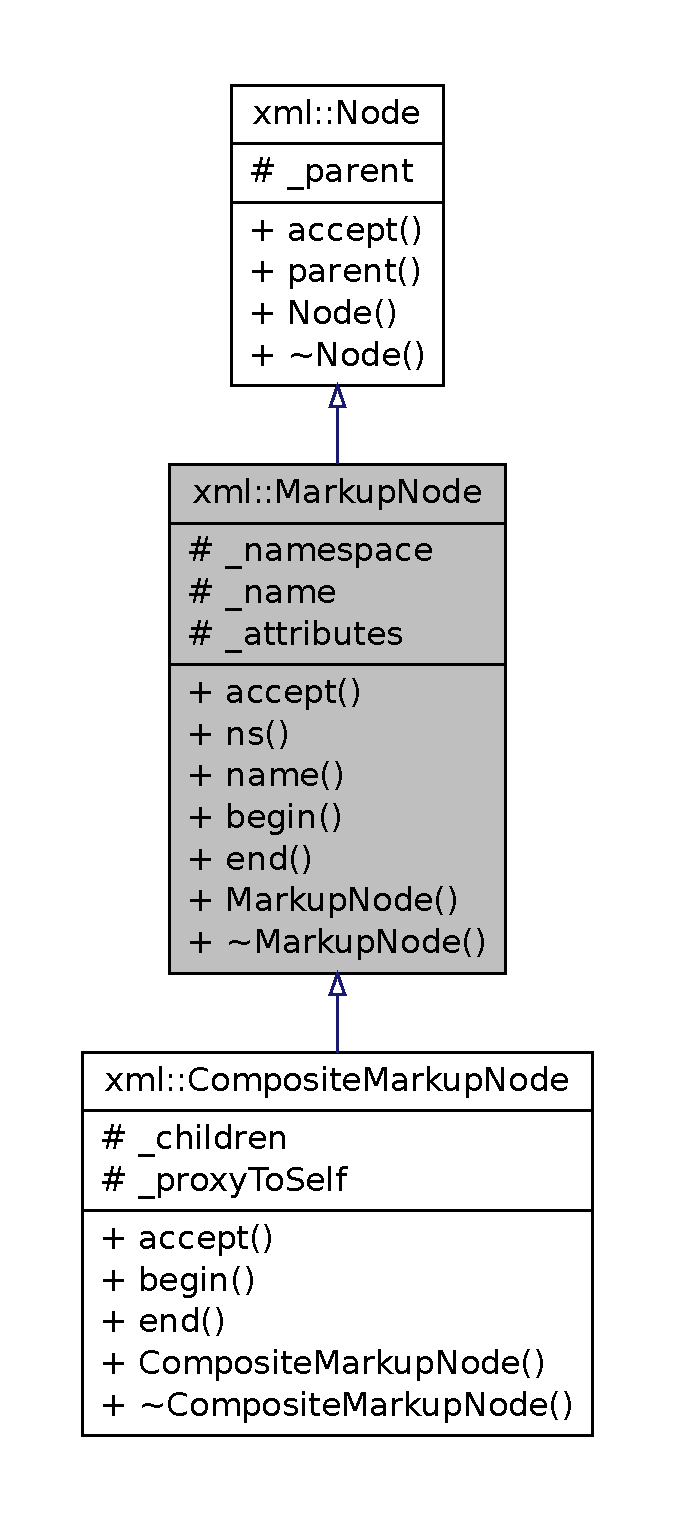
\includegraphics[height=600pt]{classxml_1_1_markup_node__inherit__graph}
\end{center}
\end{figure}


Graphe de collaboration de xml::MarkupNode:
\nopagebreak
\begin{figure}[H]
\begin{center}
\leavevmode
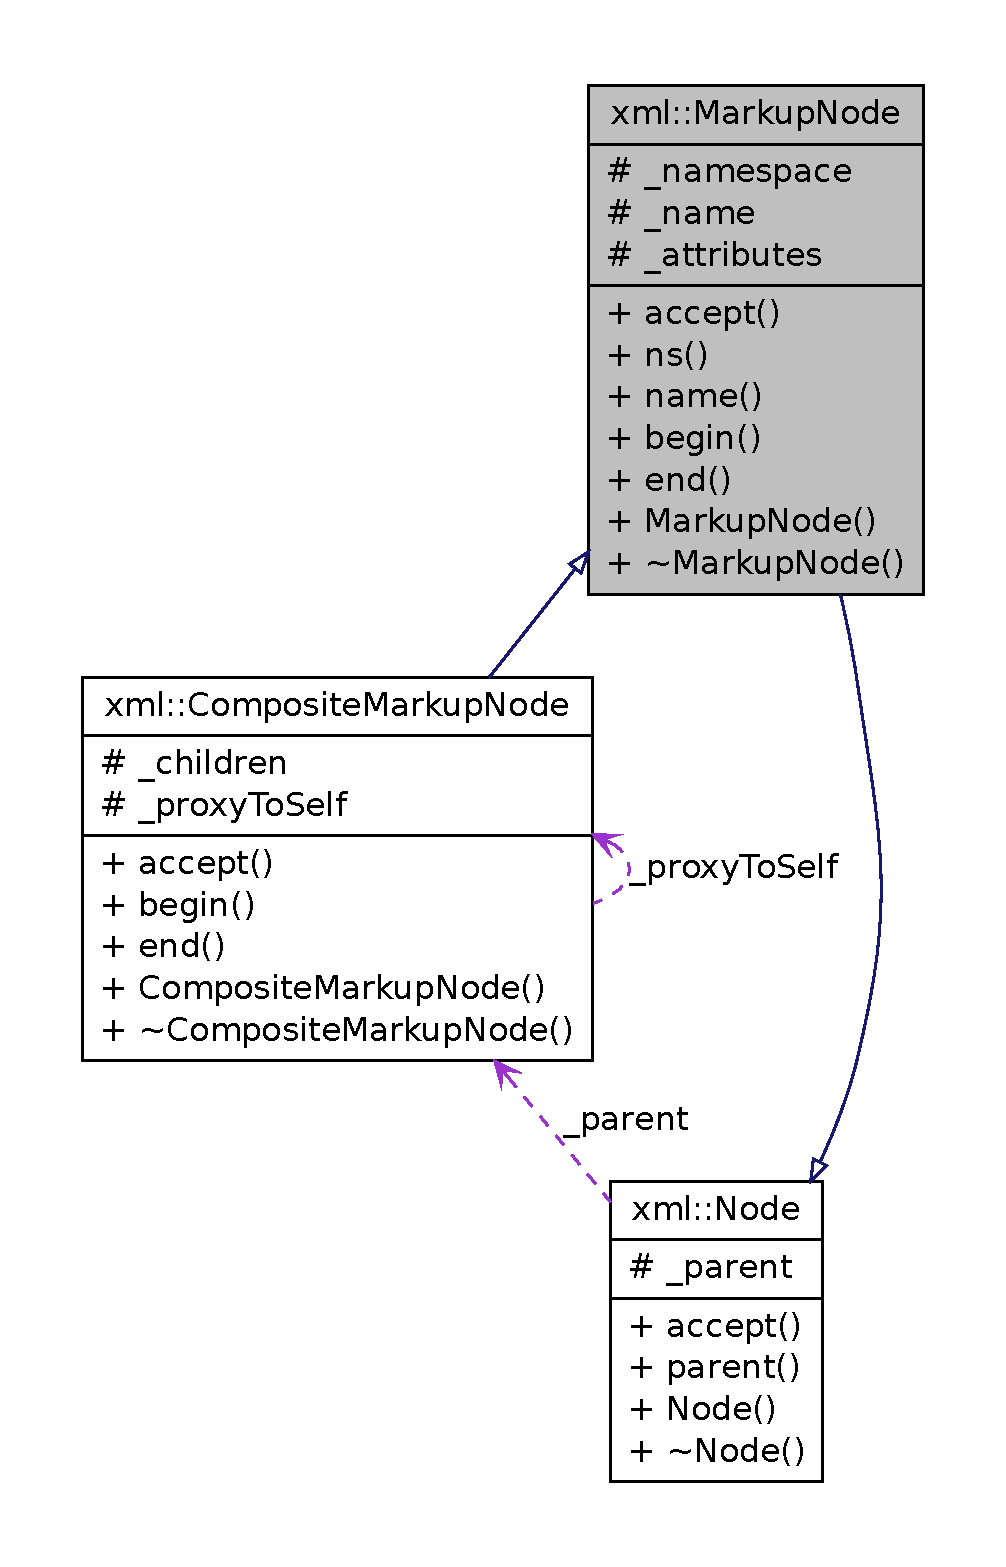
\includegraphics[height=600pt]{classxml_1_1_markup_node__coll__graph}
\end{center}
\end{figure}
\subsection*{Types publics}
\begin{DoxyCompactItemize}
\item 
typedef std::map$<$ std::string, std::string $>$ \hyperlink{classxml_1_1_markup_node_ade6f6045d18042d1a87f80f308f177fb}{Attributes}
\item 
typedef \_\-Attributes::const\_\-iterator \hyperlink{classxml_1_1_markup_node_aab83830a10c767edbed9623af05e7a3c}{AttributesIterator}
\end{DoxyCompactItemize}
\subsection*{Fonctions membres publiques}
\begin{DoxyCompactItemize}
\item 
virtual void \hyperlink{classxml_1_1_markup_node_ae70b538ce71b427c1ea552b0b41c3b34}{accept} (\hyperlink{classxml_1_1_interface_node_visitor}{InterfaceNodeVisitor} \&visitor) const 
\item 
std::string \hyperlink{classxml_1_1_markup_node_a0b5a2b37912a2957be48bbc629fc3cf9}{ns} () const 
\item 
std::string \hyperlink{classxml_1_1_markup_node_a26e3ad142b13980f2ad181ca76dfe0a9}{name} () const 
\item 
\hyperlink{classxml_1_1_markup_node_aab83830a10c767edbed9623af05e7a3c}{AttributesIterator} \hyperlink{classxml_1_1_markup_node_a48aac1f80b326393fdac05835604c69f}{begin} () const 
\item 
\hyperlink{classxml_1_1_markup_node_aab83830a10c767edbed9623af05e7a3c}{AttributesIterator} \hyperlink{classxml_1_1_markup_node_a3b63a8ea94999e2f688f6dc606f3e24b}{end} () const 
\item 
\hyperlink{classxml_1_1_markup_node_a8cc66b7a2019a38fafe0b24614ab9735}{MarkupNode} (\hyperlink{classxml_1_1_composite_markup_node}{CompositeMarkupNode} $\ast$$\ast$parent, const std::string \&ns, const std::string \&name, const \hyperlink{classxml_1_1_markup_node_ade6f6045d18042d1a87f80f308f177fb}{Attributes} \&attributes)
\item 
virtual \hyperlink{classxml_1_1_markup_node_a2067f6fd10373e45e2a98749e1384001}{$\sim$MarkupNode} ()
\end{DoxyCompactItemize}
\subsection*{Types protégés}
\begin{DoxyCompactItemize}
\item 
typedef std::map$<$ std::string, std::string $>$ \hyperlink{classxml_1_1_markup_node_a2d052c364321c4f1f506f9f17d8c8089}{\_\-Attributes}
\end{DoxyCompactItemize}
\subsection*{Attributs protégés}
\begin{DoxyCompactItemize}
\item 
std::string \hyperlink{classxml_1_1_markup_node_a18ffd5e490fc7028b580323f5892800f}{\_\-namespace}
\item 
std::string \hyperlink{classxml_1_1_markup_node_a372e14f2da008d1f2da1a5b9c8eb7600}{\_\-name}
\item 
\hyperlink{classxml_1_1_markup_node_a2d052c364321c4f1f506f9f17d8c8089}{\_\-Attributes} \hyperlink{classxml_1_1_markup_node_ada616acd43f59affa41ab7a0e6f19baf}{\_\-attributes}
\end{DoxyCompactItemize}


\subsection{Description détaillée}


Définition à la ligne 26 du fichier MarkupNode.hh.



\subsection{Documentation des définitions de type membres}
\hypertarget{classxml_1_1_markup_node_a2d052c364321c4f1f506f9f17d8c8089}{
\index{xml::MarkupNode@{xml::MarkupNode}!\_\-Attributes@{\_\-Attributes}}
\index{\_\-Attributes@{\_\-Attributes}!xml::MarkupNode@{xml::MarkupNode}}
\subsubsection[{\_\-Attributes}]{\setlength{\rightskip}{0pt plus 5cm}typedef std::map$<$std::string, std::string$>$ {\bf xml::MarkupNode::\_\-Attributes}\hspace{0.3cm}{\ttfamily  \mbox{[}protected\mbox{]}}}}
\label{classxml_1_1_markup_node_a2d052c364321c4f1f506f9f17d8c8089}


Définition à la ligne 29 du fichier MarkupNode.hh.

\hypertarget{classxml_1_1_markup_node_ade6f6045d18042d1a87f80f308f177fb}{
\index{xml::MarkupNode@{xml::MarkupNode}!Attributes@{Attributes}}
\index{Attributes@{Attributes}!xml::MarkupNode@{xml::MarkupNode}}
\subsubsection[{Attributes}]{\setlength{\rightskip}{0pt plus 5cm}typedef std::map$<$std::string, std::string$>$ {\bf xml::MarkupNode::Attributes}}}
\label{classxml_1_1_markup_node_ade6f6045d18042d1a87f80f308f177fb}


Définition à la ligne 35 du fichier MarkupNode.hh.

\hypertarget{classxml_1_1_markup_node_aab83830a10c767edbed9623af05e7a3c}{
\index{xml::MarkupNode@{xml::MarkupNode}!AttributesIterator@{AttributesIterator}}
\index{AttributesIterator@{AttributesIterator}!xml::MarkupNode@{xml::MarkupNode}}
\subsubsection[{AttributesIterator}]{\setlength{\rightskip}{0pt plus 5cm}typedef \_\-Attributes::const\_\-iterator {\bf xml::MarkupNode::AttributesIterator}}}
\label{classxml_1_1_markup_node_aab83830a10c767edbed9623af05e7a3c}


Définition à la ligne 36 du fichier MarkupNode.hh.



\subsection{Documentation des constructeurs et destructeur}
\hypertarget{classxml_1_1_markup_node_a8cc66b7a2019a38fafe0b24614ab9735}{
\index{xml::MarkupNode@{xml::MarkupNode}!MarkupNode@{MarkupNode}}
\index{MarkupNode@{MarkupNode}!xml::MarkupNode@{xml::MarkupNode}}
\subsubsection[{MarkupNode}]{\setlength{\rightskip}{0pt plus 5cm}xml::MarkupNode::MarkupNode (
\begin{DoxyParamCaption}
\item[{{\bf CompositeMarkupNode} $\ast$$\ast$}]{ parent, }
\item[{const std::string \&}]{ ns, }
\item[{const std::string \&}]{ name, }
\item[{const {\bf Attributes} \&}]{ attributes}
\end{DoxyParamCaption}
)}}
\label{classxml_1_1_markup_node_a8cc66b7a2019a38fafe0b24614ab9735}


Définition à la ligne 61 du fichier MarkupNode.cpp.

\hypertarget{classxml_1_1_markup_node_a2067f6fd10373e45e2a98749e1384001}{
\index{xml::MarkupNode@{xml::MarkupNode}!$\sim$MarkupNode@{$\sim$MarkupNode}}
\index{$\sim$MarkupNode@{$\sim$MarkupNode}!xml::MarkupNode@{xml::MarkupNode}}
\subsubsection[{$\sim$MarkupNode}]{\setlength{\rightskip}{0pt plus 5cm}xml::MarkupNode::$\sim$MarkupNode (
\begin{DoxyParamCaption}
{}
\end{DoxyParamCaption}
)\hspace{0.3cm}{\ttfamily  \mbox{[}virtual\mbox{]}}}}
\label{classxml_1_1_markup_node_a2067f6fd10373e45e2a98749e1384001}


Définition à la ligne 69 du fichier MarkupNode.cpp.



\subsection{Documentation des fonctions membres}
\hypertarget{classxml_1_1_markup_node_ae70b538ce71b427c1ea552b0b41c3b34}{
\index{xml::MarkupNode@{xml::MarkupNode}!accept@{accept}}
\index{accept@{accept}!xml::MarkupNode@{xml::MarkupNode}}
\subsubsection[{accept}]{\setlength{\rightskip}{0pt plus 5cm}void xml::MarkupNode::accept (
\begin{DoxyParamCaption}
\item[{{\bf InterfaceNodeVisitor} \&}]{ visitor}
\end{DoxyParamCaption}
) const\hspace{0.3cm}{\ttfamily  \mbox{[}virtual\mbox{]}}}}
\label{classxml_1_1_markup_node_ae70b538ce71b427c1ea552b0b41c3b34}


Implémente \hyperlink{classxml_1_1_node_a332d84602db92c390e57eeec79c4b02d}{xml::Node}.



Réimplémentée dans \hyperlink{classxml_1_1_composite_markup_node_a6c61880592cc2e911517bb3e54c3c987}{xml::CompositeMarkupNode}.



Définition à la ligne 32 du fichier MarkupNode.cpp.



Voici le graphe d'appel pour cette fonction :
\nopagebreak
\begin{figure}[H]
\begin{center}
\leavevmode
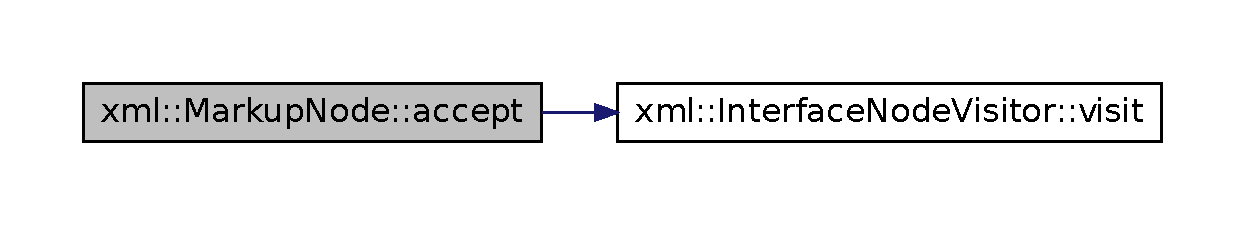
\includegraphics[width=400pt]{classxml_1_1_markup_node_ae70b538ce71b427c1ea552b0b41c3b34_cgraph}
\end{center}
\end{figure}


\hypertarget{classxml_1_1_markup_node_a48aac1f80b326393fdac05835604c69f}{
\index{xml::MarkupNode@{xml::MarkupNode}!begin@{begin}}
\index{begin@{begin}!xml::MarkupNode@{xml::MarkupNode}}
\subsubsection[{begin}]{\setlength{\rightskip}{0pt plus 5cm}{\bf MarkupNode::AttributesIterator} xml::MarkupNode::begin (
\begin{DoxyParamCaption}
{}
\end{DoxyParamCaption}
) const}}
\label{classxml_1_1_markup_node_a48aac1f80b326393fdac05835604c69f}


Réimplémentée dans \hyperlink{classxml_1_1_composite_markup_node_a124753f641dc4612cee80fd289bf68a6}{xml::CompositeMarkupNode}.



Définition à la ligne 47 du fichier MarkupNode.cpp.

\hypertarget{classxml_1_1_markup_node_a3b63a8ea94999e2f688f6dc606f3e24b}{
\index{xml::MarkupNode@{xml::MarkupNode}!end@{end}}
\index{end@{end}!xml::MarkupNode@{xml::MarkupNode}}
\subsubsection[{end}]{\setlength{\rightskip}{0pt plus 5cm}{\bf MarkupNode::AttributesIterator} xml::MarkupNode::end (
\begin{DoxyParamCaption}
{}
\end{DoxyParamCaption}
) const}}
\label{classxml_1_1_markup_node_a3b63a8ea94999e2f688f6dc606f3e24b}


Réimplémentée dans \hyperlink{classxml_1_1_composite_markup_node_aeebeee1fc877fe102bad454d2ffa5bba}{xml::CompositeMarkupNode}.



Définition à la ligne 52 du fichier MarkupNode.cpp.

\hypertarget{classxml_1_1_markup_node_a26e3ad142b13980f2ad181ca76dfe0a9}{
\index{xml::MarkupNode@{xml::MarkupNode}!name@{name}}
\index{name@{name}!xml::MarkupNode@{xml::MarkupNode}}
\subsubsection[{name}]{\setlength{\rightskip}{0pt plus 5cm}string xml::MarkupNode::name (
\begin{DoxyParamCaption}
{}
\end{DoxyParamCaption}
) const}}
\label{classxml_1_1_markup_node_a26e3ad142b13980f2ad181ca76dfe0a9}


Définition à la ligne 42 du fichier MarkupNode.cpp.

\hypertarget{classxml_1_1_markup_node_a0b5a2b37912a2957be48bbc629fc3cf9}{
\index{xml::MarkupNode@{xml::MarkupNode}!ns@{ns}}
\index{ns@{ns}!xml::MarkupNode@{xml::MarkupNode}}
\subsubsection[{ns}]{\setlength{\rightskip}{0pt plus 5cm}string xml::MarkupNode::ns (
\begin{DoxyParamCaption}
{}
\end{DoxyParamCaption}
) const}}
\label{classxml_1_1_markup_node_a0b5a2b37912a2957be48bbc629fc3cf9}


Définition à la ligne 37 du fichier MarkupNode.cpp.



\subsection{Documentation des données membres}
\hypertarget{classxml_1_1_markup_node_ada616acd43f59affa41ab7a0e6f19baf}{
\index{xml::MarkupNode@{xml::MarkupNode}!\_\-attributes@{\_\-attributes}}
\index{\_\-attributes@{\_\-attributes}!xml::MarkupNode@{xml::MarkupNode}}
\subsubsection[{\_\-attributes}]{\setlength{\rightskip}{0pt plus 5cm}{\bf \_\-Attributes} {\bf xml::MarkupNode::\_\-attributes}\hspace{0.3cm}{\ttfamily  \mbox{[}protected\mbox{]}}}}
\label{classxml_1_1_markup_node_ada616acd43f59affa41ab7a0e6f19baf}


Définition à la ligne 102 du fichier MarkupNode.hh.

\hypertarget{classxml_1_1_markup_node_a372e14f2da008d1f2da1a5b9c8eb7600}{
\index{xml::MarkupNode@{xml::MarkupNode}!\_\-name@{\_\-name}}
\index{\_\-name@{\_\-name}!xml::MarkupNode@{xml::MarkupNode}}
\subsubsection[{\_\-name}]{\setlength{\rightskip}{0pt plus 5cm}std::string {\bf xml::MarkupNode::\_\-name}\hspace{0.3cm}{\ttfamily  \mbox{[}protected\mbox{]}}}}
\label{classxml_1_1_markup_node_a372e14f2da008d1f2da1a5b9c8eb7600}


Définition à la ligne 101 du fichier MarkupNode.hh.

\hypertarget{classxml_1_1_markup_node_a18ffd5e490fc7028b580323f5892800f}{
\index{xml::MarkupNode@{xml::MarkupNode}!\_\-namespace@{\_\-namespace}}
\index{\_\-namespace@{\_\-namespace}!xml::MarkupNode@{xml::MarkupNode}}
\subsubsection[{\_\-namespace}]{\setlength{\rightskip}{0pt plus 5cm}std::string {\bf xml::MarkupNode::\_\-namespace}\hspace{0.3cm}{\ttfamily  \mbox{[}protected\mbox{]}}}}
\label{classxml_1_1_markup_node_a18ffd5e490fc7028b580323f5892800f}


Définition à la ligne 100 du fichier MarkupNode.hh.



La documentation de cette classe a été générée à partir des fichiers suivants :\begin{DoxyCompactItemize}
\item 
src/\hyperlink{_markup_node_8hh}{MarkupNode.hh}\item 
src/\hyperlink{_markup_node_8cpp}{MarkupNode.cpp}\end{DoxyCompactItemize}

\hypertarget{classxml_1_1_node}{
\section{Référence de la classe xml::Node}
\label{classxml_1_1_node}\index{xml::Node@{xml::Node}}
}


{\ttfamily \#include $<$Node.hh$>$}



Graphe d'héritage de xml::Node:
\nopagebreak
\begin{figure}[H]
\begin{center}
\leavevmode
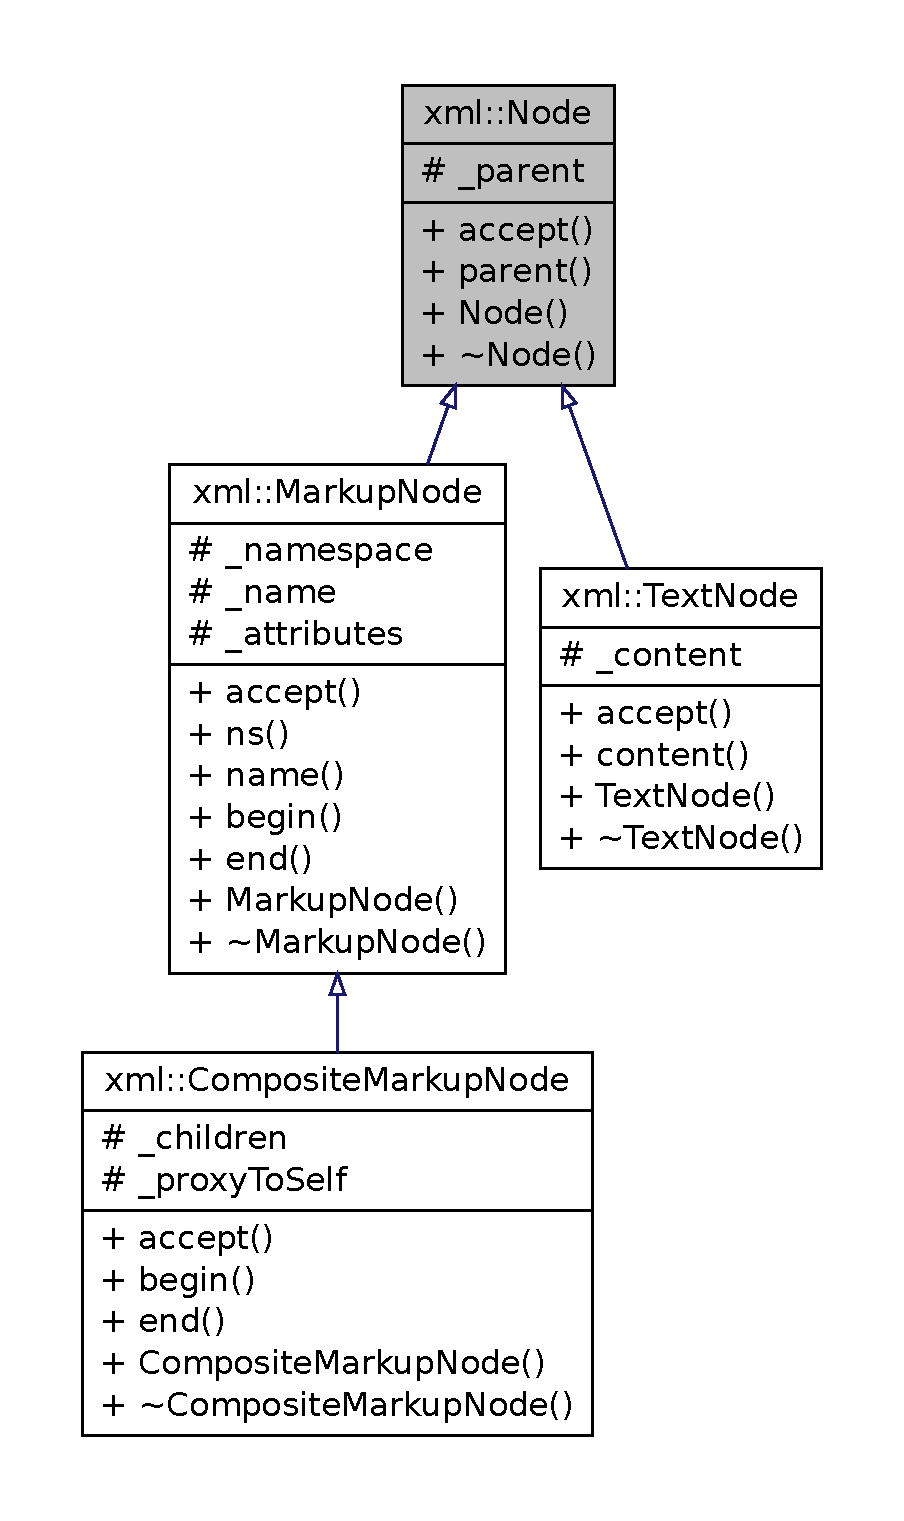
\includegraphics[height=600pt]{classxml_1_1_node__inherit__graph}
\end{center}
\end{figure}


Graphe de collaboration de xml::Node:
\nopagebreak
\begin{figure}[H]
\begin{center}
\leavevmode
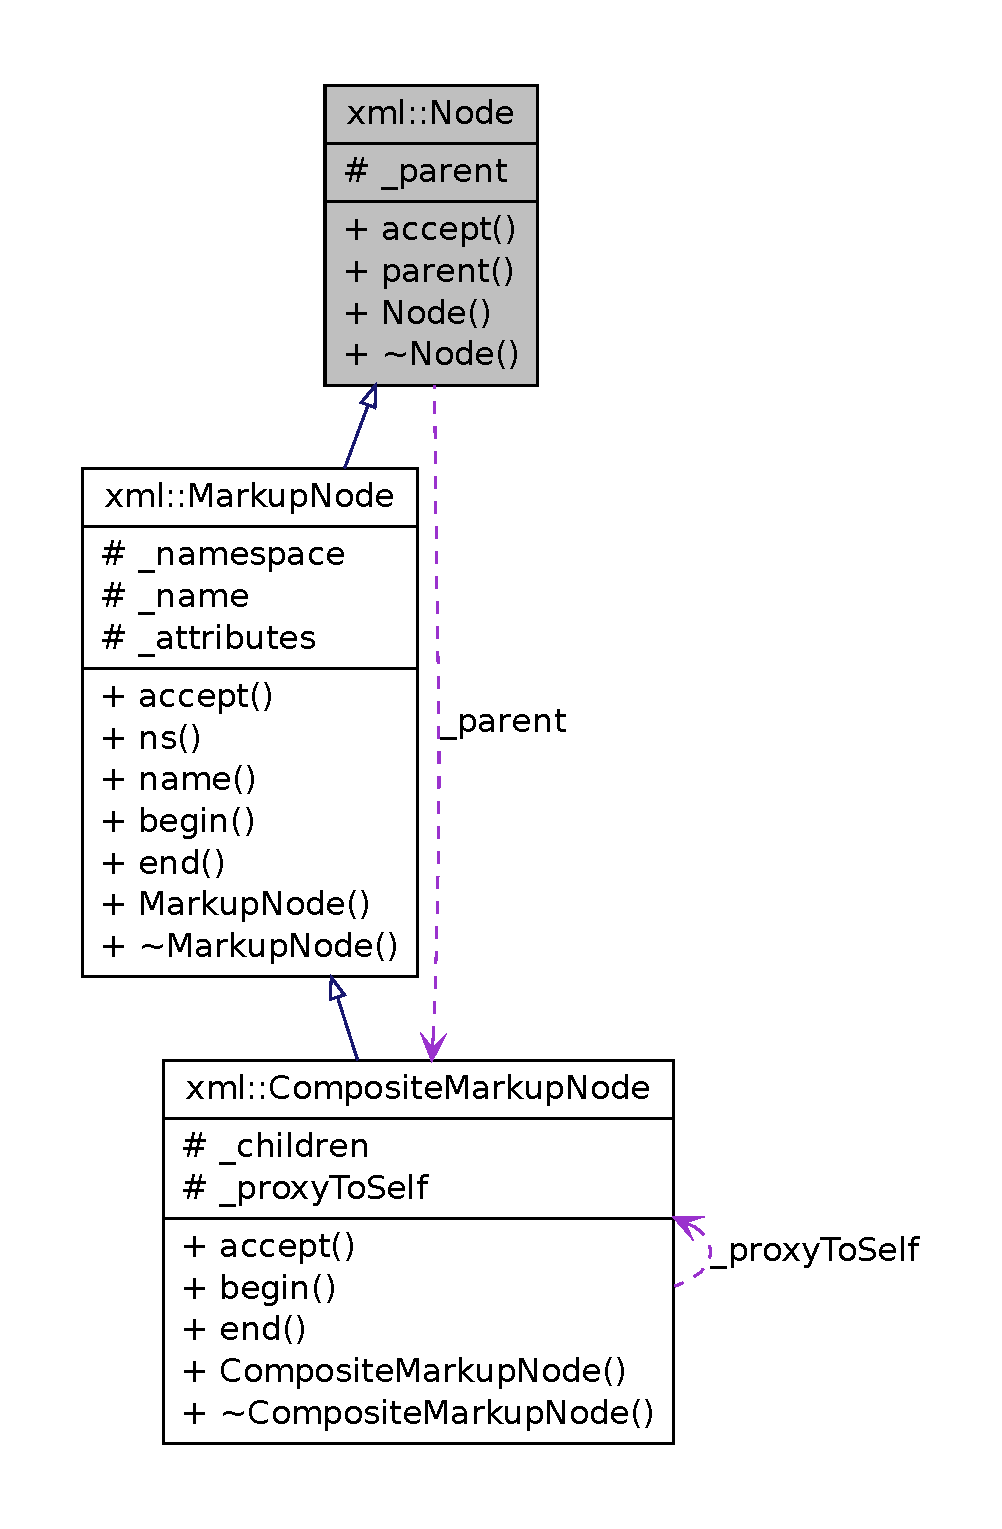
\includegraphics[height=600pt]{classxml_1_1_node__coll__graph}
\end{center}
\end{figure}
\subsection*{Fonctions membres publiques}
\begin{DoxyCompactItemize}
\item 
virtual void \hyperlink{classxml_1_1_node_a332d84602db92c390e57eeec79c4b02d}{accept} (\hyperlink{classxml_1_1_interface_node_visitor}{InterfaceNodeVisitor} \&visitor) const =0
\item 
\hyperlink{classxml_1_1_node}{Node} $\ast$ \hyperlink{classxml_1_1_node_a7b316f796ec1a98f127b6f9e0802b579}{parent} () const 
\item 
\hyperlink{classxml_1_1_node_a79b919ce53463d9b63ad38b6bb934c63}{Node} (\hyperlink{classxml_1_1_composite_markup_node}{CompositeMarkupNode} $\ast$$\ast$parent)
\item 
virtual \hyperlink{classxml_1_1_node_a4529378ae3f081120e846c9d44154f92}{$\sim$Node} ()
\end{DoxyCompactItemize}
\subsection*{Attributs protégés}
\begin{DoxyCompactItemize}
\item 
\hyperlink{classxml_1_1_composite_markup_node}{CompositeMarkupNode} $\ast$$\ast$ \hyperlink{classxml_1_1_node_afd48d71b81dba400788d0a0367b5c478}{\_\-parent}
\end{DoxyCompactItemize}


\subsection{Description détaillée}


Définition à la ligne 26 du fichier Node.hh.



\subsection{Documentation des constructeurs et destructeur}
\hypertarget{classxml_1_1_node_a79b919ce53463d9b63ad38b6bb934c63}{
\index{xml::Node@{xml::Node}!Node@{Node}}
\index{Node@{Node}!xml::Node@{xml::Node}}
\subsubsection[{Node}]{\setlength{\rightskip}{0pt plus 5cm}xml::Node::Node (
\begin{DoxyParamCaption}
\item[{{\bf CompositeMarkupNode} $\ast$$\ast$}]{ parent}
\end{DoxyParamCaption}
)}}
\label{classxml_1_1_node_a79b919ce53463d9b63ad38b6bb934c63}


Définition à la ligne 45 du fichier Node.cpp.

\hypertarget{classxml_1_1_node_a4529378ae3f081120e846c9d44154f92}{
\index{xml::Node@{xml::Node}!$\sim$Node@{$\sim$Node}}
\index{$\sim$Node@{$\sim$Node}!xml::Node@{xml::Node}}
\subsubsection[{$\sim$Node}]{\setlength{\rightskip}{0pt plus 5cm}xml::Node::$\sim$Node (
\begin{DoxyParamCaption}
{}
\end{DoxyParamCaption}
)\hspace{0.3cm}{\ttfamily  \mbox{[}virtual\mbox{]}}}}
\label{classxml_1_1_node_a4529378ae3f081120e846c9d44154f92}


Définition à la ligne 51 du fichier Node.cpp.



\subsection{Documentation des fonctions membres}
\hypertarget{classxml_1_1_node_a332d84602db92c390e57eeec79c4b02d}{
\index{xml::Node@{xml::Node}!accept@{accept}}
\index{accept@{accept}!xml::Node@{xml::Node}}
\subsubsection[{accept}]{\setlength{\rightskip}{0pt plus 5cm}virtual void xml::Node::accept (
\begin{DoxyParamCaption}
\item[{{\bf InterfaceNodeVisitor} \&}]{ visitor}
\end{DoxyParamCaption}
) const\hspace{0.3cm}{\ttfamily  \mbox{[}pure virtual\mbox{]}}}}
\label{classxml_1_1_node_a332d84602db92c390e57eeec79c4b02d}


Implémenté dans \hyperlink{classxml_1_1_composite_markup_node_a6c61880592cc2e911517bb3e54c3c987}{xml::CompositeMarkupNode}, \hyperlink{classxml_1_1_markup_node_ae70b538ce71b427c1ea552b0b41c3b34}{xml::MarkupNode}, et \hyperlink{classxml_1_1_text_node_ac918f8f74e141690e18cd8e23d174996}{xml::TextNode}.

\hypertarget{classxml_1_1_node_a7b316f796ec1a98f127b6f9e0802b579}{
\index{xml::Node@{xml::Node}!parent@{parent}}
\index{parent@{parent}!xml::Node@{xml::Node}}
\subsubsection[{parent}]{\setlength{\rightskip}{0pt plus 5cm}{\bf Node} $\ast$ xml::Node::parent (
\begin{DoxyParamCaption}
{}
\end{DoxyParamCaption}
) const}}
\label{classxml_1_1_node_a7b316f796ec1a98f127b6f9e0802b579}


Définition à la ligne 33 du fichier Node.cpp.



\subsection{Documentation des données membres}
\hypertarget{classxml_1_1_node_afd48d71b81dba400788d0a0367b5c478}{
\index{xml::Node@{xml::Node}!\_\-parent@{\_\-parent}}
\index{\_\-parent@{\_\-parent}!xml::Node@{xml::Node}}
\subsubsection[{\_\-parent}]{\setlength{\rightskip}{0pt plus 5cm}{\bf CompositeMarkupNode}$\ast$$\ast$ {\bf xml::Node::\_\-parent}\hspace{0.3cm}{\ttfamily  \mbox{[}protected\mbox{]}}}}
\label{classxml_1_1_node_afd48d71b81dba400788d0a0367b5c478}


Définition à la ligne 67 du fichier Node.hh.



La documentation de cette classe a été générée à partir des fichiers suivants :\begin{DoxyCompactItemize}
\item 
src/\hyperlink{_node_8hh}{Node.hh}\item 
src/\hyperlink{_node_8cpp}{Node.cpp}\end{DoxyCompactItemize}

\hypertarget{classxml_1_1_output_visitor}{
\section{Référence de la classe xml::OutputVisitor}
\label{classxml_1_1_output_visitor}\index{xml::OutputVisitor@{xml::OutputVisitor}}
}


{\ttfamily \#include $<$OutputVisitor.hh$>$}



Graphe d'héritage de xml::OutputVisitor:
\nopagebreak
\begin{figure}[H]
\begin{center}
\leavevmode
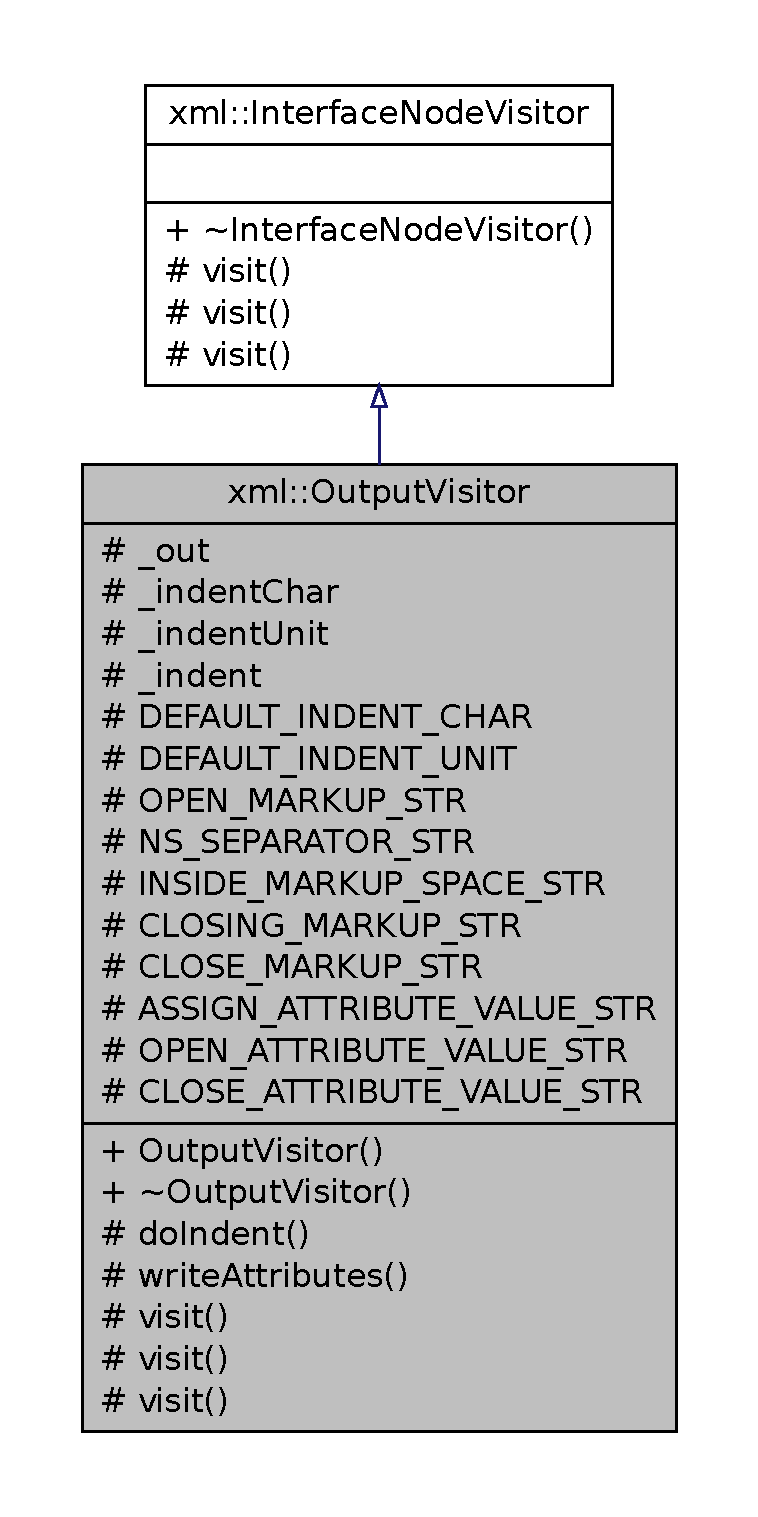
\includegraphics[height=600pt]{classxml_1_1_output_visitor__inherit__graph}
\end{center}
\end{figure}


Graphe de collaboration de xml::OutputVisitor:
\nopagebreak
\begin{figure}[H]
\begin{center}
\leavevmode
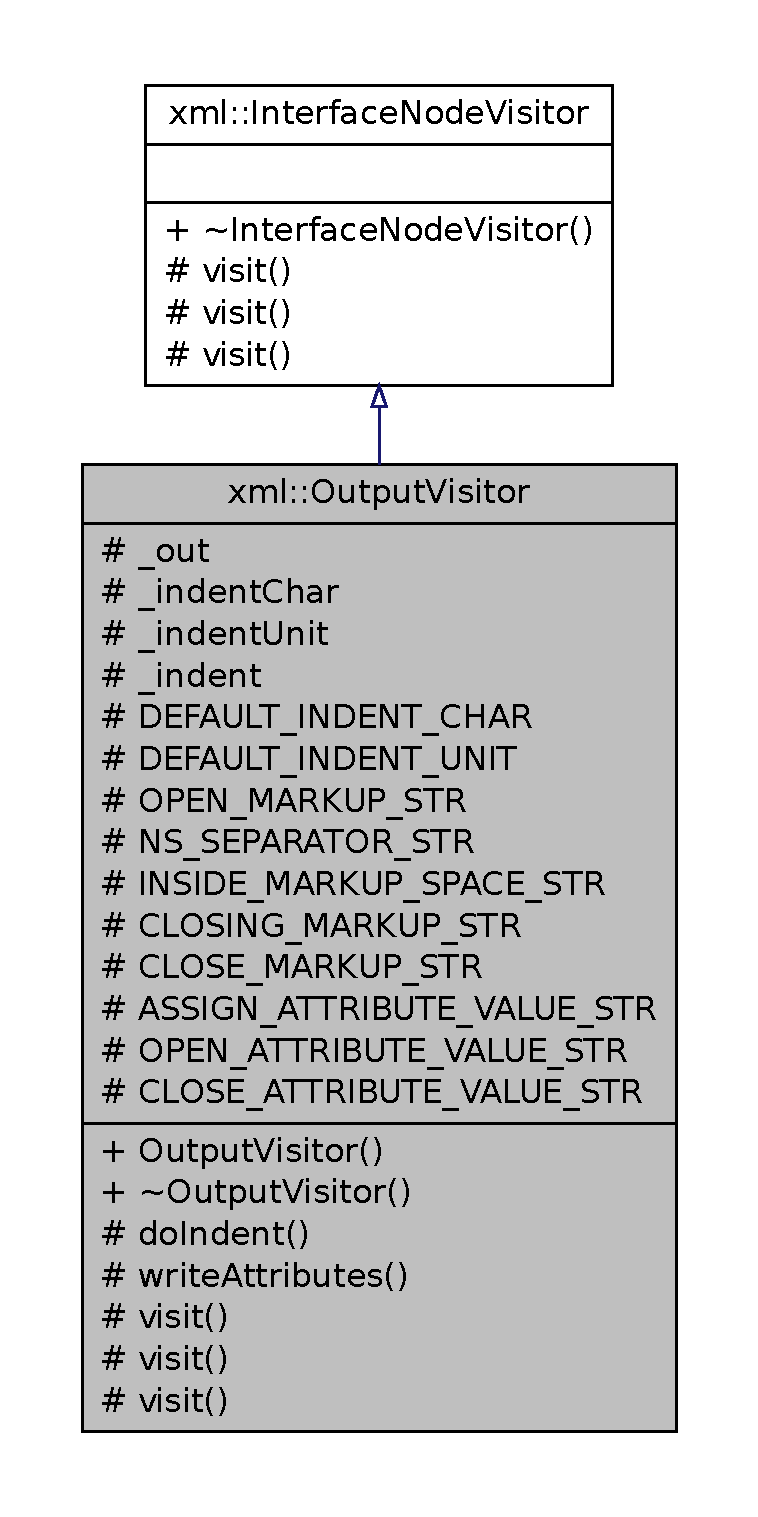
\includegraphics[height=600pt]{classxml_1_1_output_visitor__coll__graph}
\end{center}
\end{figure}
\subsection*{Fonctions membres publiques}
\begin{DoxyCompactItemize}
\item 
\hyperlink{classxml_1_1_output_visitor_a09e8e0dd6ac2bbbf39cab4fa79a65a4b}{OutputVisitor} (std::ostream \&out, char indentChar=\hyperlink{classxml_1_1_output_visitor_ad61c526a1962865b37f22fdf252b63f3}{DEFAULT\_\-INDENT\_\-CHAR}, unsigned int indentUnit=\hyperlink{classxml_1_1_output_visitor_aa5e9426f0fdf70d3e0922837c8c99f93}{DEFAULT\_\-INDENT\_\-UNIT})
\item 
virtual \hyperlink{classxml_1_1_output_visitor_a6143fdb2f73ab2bafa7f2b3e3c32e48a}{$\sim$OutputVisitor} ()
\end{DoxyCompactItemize}
\subsection*{Fonctions membres protégées}
\begin{DoxyCompactItemize}
\item 
void \hyperlink{classxml_1_1_output_visitor_af369ea5f7984975e7dfdea89ddcae000}{doIndent} ()
\item 
void \hyperlink{classxml_1_1_output_visitor_a3c1d2ac6dec2c9f6279a59226646e254}{writeAttributes} (const \hyperlink{classxml_1_1_markup_node}{MarkupNode} \&node)
\item 
virtual void \hyperlink{classxml_1_1_output_visitor_a33e53f866b31a155bbf29ffda852aaf7}{visit} (const \hyperlink{classxml_1_1_text_node}{TextNode} \&node)
\item 
virtual void \hyperlink{classxml_1_1_output_visitor_ac1dae5dbb561c4b7e98a761d5d503e49}{visit} (const \hyperlink{classxml_1_1_markup_node}{MarkupNode} \&node)
\item 
virtual void \hyperlink{classxml_1_1_output_visitor_addfc73ae3643a8285b5f892eff1a6066}{visit} (const \hyperlink{classxml_1_1_composite_markup_node}{CompositeMarkupNode} \&node)
\end{DoxyCompactItemize}
\subsection*{Attributs protégés}
\begin{DoxyCompactItemize}
\item 
std::ostream \& \hyperlink{classxml_1_1_output_visitor_ab2e31d8a9675f88d96a89399ea894e83}{\_\-out}
\item 
char \hyperlink{classxml_1_1_output_visitor_a9b89adad1ba1e3ff2f64ad7cd6545361}{\_\-indentChar}
\item 
unsigned \hyperlink{classxml_1_1_output_visitor_a55060d8246a1365089872aa4a500b03c}{\_\-indentUnit}
\item 
unsigned int \hyperlink{classxml_1_1_output_visitor_a7664b7975557ab6db96b744bf43190f4}{\_\-indent}
\end{DoxyCompactItemize}
\subsection*{Attributs protégés statiques}
\begin{DoxyCompactItemize}
\item 
static const char \hyperlink{classxml_1_1_output_visitor_ad61c526a1962865b37f22fdf252b63f3}{DEFAULT\_\-INDENT\_\-CHAR} = ' '
\item 
static const unsigned char \hyperlink{classxml_1_1_output_visitor_aa5e9426f0fdf70d3e0922837c8c99f93}{DEFAULT\_\-INDENT\_\-UNIT} = 1
\item 
static const std::string \hyperlink{classxml_1_1_output_visitor_a3a2a1c7860151f173fd28c0077ffd94a}{OPEN\_\-MARKUP\_\-STR} = \char`\"{}$<$\char`\"{}
\item 
static const std::string \hyperlink{classxml_1_1_output_visitor_a892952bcc6a8b9265c0934cfdc95dd65}{NS\_\-SEPARATOR\_\-STR} = \char`\"{}:\char`\"{}
\item 
static const std::string \hyperlink{classxml_1_1_output_visitor_a67d0548ce8906eb4121d9f33d005c8be}{INSIDE\_\-MARKUP\_\-SPACE\_\-STR} = \char`\"{} \char`\"{}
\item 
static const std::string \hyperlink{classxml_1_1_output_visitor_af06f2eb91d0a40d0d090aeb0bdeb9c9f}{CLOSING\_\-MARKUP\_\-STR} = \char`\"{}/\char`\"{}
\item 
static const std::string \hyperlink{classxml_1_1_output_visitor_aef349142e7de8a309ee5dd048cc5b51f}{CLOSE\_\-MARKUP\_\-STR} = \char`\"{}$>$\char`\"{}
\item 
static const std::string \hyperlink{classxml_1_1_output_visitor_a7eb4bfa043240d8d87fe47eb733057c4}{ASSIGN\_\-ATTRIBUTE\_\-VALUE\_\-STR} = \char`\"{}=\char`\"{}
\item 
static const std::string \hyperlink{classxml_1_1_output_visitor_a16ae3df2d90ed3e57ea51277de609988}{OPEN\_\-ATTRIBUTE\_\-VALUE\_\-STR} = \char`\"{}$\backslash$\char`\"{}\char`\"{}
\item 
static const std::string \hyperlink{classxml_1_1_output_visitor_af3b7b1a653908df91dc19195b3bdb29b}{CLOSE\_\-ATTRIBUTE\_\-VALUE\_\-STR} = \char`\"{}$\backslash$\char`\"{}\char`\"{}
\end{DoxyCompactItemize}


\subsection{Description détaillée}


Définition à la ligne 24 du fichier OutputVisitor.hh.



\subsection{Documentation des constructeurs et destructeur}
\hypertarget{classxml_1_1_output_visitor_a09e8e0dd6ac2bbbf39cab4fa79a65a4b}{
\index{xml::OutputVisitor@{xml::OutputVisitor}!OutputVisitor@{OutputVisitor}}
\index{OutputVisitor@{OutputVisitor}!xml::OutputVisitor@{xml::OutputVisitor}}
\subsubsection[{OutputVisitor}]{\setlength{\rightskip}{0pt plus 5cm}xml::OutputVisitor::OutputVisitor (
\begin{DoxyParamCaption}
\item[{std::ostream \&}]{ out, }
\item[{char}]{ indentChar = {\ttfamily {\bf DEFAULT\_\-INDENT\_\-CHAR}}, }
\item[{unsigned int}]{ indentUnit = {\ttfamily {\bf DEFAULT\_\-INDENT\_\-UNIT}}}
\end{DoxyParamCaption}
)}}
\label{classxml_1_1_output_visitor_a09e8e0dd6ac2bbbf39cab4fa79a65a4b}
\hypertarget{classxml_1_1_output_visitor_a6143fdb2f73ab2bafa7f2b3e3c32e48a}{
\index{xml::OutputVisitor@{xml::OutputVisitor}!$\sim$OutputVisitor@{$\sim$OutputVisitor}}
\index{$\sim$OutputVisitor@{$\sim$OutputVisitor}!xml::OutputVisitor@{xml::OutputVisitor}}
\subsubsection[{$\sim$OutputVisitor}]{\setlength{\rightskip}{0pt plus 5cm}xml::OutputVisitor::$\sim$OutputVisitor (
\begin{DoxyParamCaption}
{}
\end{DoxyParamCaption}
)\hspace{0.3cm}{\ttfamily  \mbox{[}virtual\mbox{]}}}}
\label{classxml_1_1_output_visitor_a6143fdb2f73ab2bafa7f2b3e3c32e48a}


Définition à la ligne 53 du fichier OutputVisitor.cpp.



\subsection{Documentation des fonctions membres}
\hypertarget{classxml_1_1_output_visitor_af369ea5f7984975e7dfdea89ddcae000}{
\index{xml::OutputVisitor@{xml::OutputVisitor}!doIndent@{doIndent}}
\index{doIndent@{doIndent}!xml::OutputVisitor@{xml::OutputVisitor}}
\subsubsection[{doIndent}]{\setlength{\rightskip}{0pt plus 5cm}void xml::OutputVisitor::doIndent (
\begin{DoxyParamCaption}
{}
\end{DoxyParamCaption}
)\hspace{0.3cm}{\ttfamily  \mbox{[}protected\mbox{]}}}}
\label{classxml_1_1_output_visitor_af369ea5f7984975e7dfdea89ddcae000}


Définition à la ligne 63 du fichier OutputVisitor.cpp.

\hypertarget{classxml_1_1_output_visitor_addfc73ae3643a8285b5f892eff1a6066}{
\index{xml::OutputVisitor@{xml::OutputVisitor}!visit@{visit}}
\index{visit@{visit}!xml::OutputVisitor@{xml::OutputVisitor}}
\subsubsection[{visit}]{\setlength{\rightskip}{0pt plus 5cm}void xml::OutputVisitor::visit (
\begin{DoxyParamCaption}
\item[{const {\bf CompositeMarkupNode} \&}]{ node}
\end{DoxyParamCaption}
)\hspace{0.3cm}{\ttfamily  \mbox{[}protected, virtual\mbox{]}}}}
\label{classxml_1_1_output_visitor_addfc73ae3643a8285b5f892eff1a6066}


Implémente \hyperlink{classxml_1_1_interface_node_visitor_afd6306ffd03380f21f436234b314c34d}{xml::InterfaceNodeVisitor}.



Définition à la ligne 97 du fichier OutputVisitor.cpp.

\hypertarget{classxml_1_1_output_visitor_ac1dae5dbb561c4b7e98a761d5d503e49}{
\index{xml::OutputVisitor@{xml::OutputVisitor}!visit@{visit}}
\index{visit@{visit}!xml::OutputVisitor@{xml::OutputVisitor}}
\subsubsection[{visit}]{\setlength{\rightskip}{0pt plus 5cm}void xml::OutputVisitor::visit (
\begin{DoxyParamCaption}
\item[{const {\bf MarkupNode} \&}]{ node}
\end{DoxyParamCaption}
)\hspace{0.3cm}{\ttfamily  \mbox{[}protected, virtual\mbox{]}}}}
\label{classxml_1_1_output_visitor_ac1dae5dbb561c4b7e98a761d5d503e49}


Implémente \hyperlink{classxml_1_1_interface_node_visitor_a53b33aabb8a79d4b1715c7664671d326}{xml::InterfaceNodeVisitor}.



Définition à la ligne 89 du fichier OutputVisitor.cpp.

\hypertarget{classxml_1_1_output_visitor_a33e53f866b31a155bbf29ffda852aaf7}{
\index{xml::OutputVisitor@{xml::OutputVisitor}!visit@{visit}}
\index{visit@{visit}!xml::OutputVisitor@{xml::OutputVisitor}}
\subsubsection[{visit}]{\setlength{\rightskip}{0pt plus 5cm}void xml::OutputVisitor::visit (
\begin{DoxyParamCaption}
\item[{const {\bf TextNode} \&}]{ node}
\end{DoxyParamCaption}
)\hspace{0.3cm}{\ttfamily  \mbox{[}protected, virtual\mbox{]}}}}
\label{classxml_1_1_output_visitor_a33e53f866b31a155bbf29ffda852aaf7}


Implémente \hyperlink{classxml_1_1_interface_node_visitor_a22a8a333e5cf2da1f1ac9f8f1f376a89}{xml::InterfaceNodeVisitor}.



Définition à la ligne 83 du fichier OutputVisitor.cpp.

\hypertarget{classxml_1_1_output_visitor_a3c1d2ac6dec2c9f6279a59226646e254}{
\index{xml::OutputVisitor@{xml::OutputVisitor}!writeAttributes@{writeAttributes}}
\index{writeAttributes@{writeAttributes}!xml::OutputVisitor@{xml::OutputVisitor}}
\subsubsection[{writeAttributes}]{\setlength{\rightskip}{0pt plus 5cm}void xml::OutputVisitor::writeAttributes (
\begin{DoxyParamCaption}
\item[{const {\bf MarkupNode} \&}]{ node}
\end{DoxyParamCaption}
)\hspace{0.3cm}{\ttfamily  \mbox{[}protected\mbox{]}}}}
\label{classxml_1_1_output_visitor_a3c1d2ac6dec2c9f6279a59226646e254}


Définition à la ligne 73 du fichier OutputVisitor.cpp.



\subsection{Documentation des données membres}
\hypertarget{classxml_1_1_output_visitor_a7664b7975557ab6db96b744bf43190f4}{
\index{xml::OutputVisitor@{xml::OutputVisitor}!\_\-indent@{\_\-indent}}
\index{\_\-indent@{\_\-indent}!xml::OutputVisitor@{xml::OutputVisitor}}
\subsubsection[{\_\-indent}]{\setlength{\rightskip}{0pt plus 5cm}unsigned int {\bf xml::OutputVisitor::\_\-indent}\hspace{0.3cm}{\ttfamily  \mbox{[}protected\mbox{]}}}}
\label{classxml_1_1_output_visitor_a7664b7975557ab6db96b744bf43190f4}


Définition à la ligne 68 du fichier OutputVisitor.hh.

\hypertarget{classxml_1_1_output_visitor_a9b89adad1ba1e3ff2f64ad7cd6545361}{
\index{xml::OutputVisitor@{xml::OutputVisitor}!\_\-indentChar@{\_\-indentChar}}
\index{\_\-indentChar@{\_\-indentChar}!xml::OutputVisitor@{xml::OutputVisitor}}
\subsubsection[{\_\-indentChar}]{\setlength{\rightskip}{0pt plus 5cm}char {\bf xml::OutputVisitor::\_\-indentChar}\hspace{0.3cm}{\ttfamily  \mbox{[}protected\mbox{]}}}}
\label{classxml_1_1_output_visitor_a9b89adad1ba1e3ff2f64ad7cd6545361}


Définition à la ligne 66 du fichier OutputVisitor.hh.

\hypertarget{classxml_1_1_output_visitor_a55060d8246a1365089872aa4a500b03c}{
\index{xml::OutputVisitor@{xml::OutputVisitor}!\_\-indentUnit@{\_\-indentUnit}}
\index{\_\-indentUnit@{\_\-indentUnit}!xml::OutputVisitor@{xml::OutputVisitor}}
\subsubsection[{\_\-indentUnit}]{\setlength{\rightskip}{0pt plus 5cm}unsigned {\bf xml::OutputVisitor::\_\-indentUnit}\hspace{0.3cm}{\ttfamily  \mbox{[}protected\mbox{]}}}}
\label{classxml_1_1_output_visitor_a55060d8246a1365089872aa4a500b03c}


Définition à la ligne 67 du fichier OutputVisitor.hh.

\hypertarget{classxml_1_1_output_visitor_ab2e31d8a9675f88d96a89399ea894e83}{
\index{xml::OutputVisitor@{xml::OutputVisitor}!\_\-out@{\_\-out}}
\index{\_\-out@{\_\-out}!xml::OutputVisitor@{xml::OutputVisitor}}
\subsubsection[{\_\-out}]{\setlength{\rightskip}{0pt plus 5cm}std::ostream\& {\bf xml::OutputVisitor::\_\-out}\hspace{0.3cm}{\ttfamily  \mbox{[}protected\mbox{]}}}}
\label{classxml_1_1_output_visitor_ab2e31d8a9675f88d96a89399ea894e83}


Définition à la ligne 65 du fichier OutputVisitor.hh.

\hypertarget{classxml_1_1_output_visitor_a7eb4bfa043240d8d87fe47eb733057c4}{
\index{xml::OutputVisitor@{xml::OutputVisitor}!ASSIGN\_\-ATTRIBUTE\_\-VALUE\_\-STR@{ASSIGN\_\-ATTRIBUTE\_\-VALUE\_\-STR}}
\index{ASSIGN\_\-ATTRIBUTE\_\-VALUE\_\-STR@{ASSIGN\_\-ATTRIBUTE\_\-VALUE\_\-STR}!xml::OutputVisitor@{xml::OutputVisitor}}
\subsubsection[{ASSIGN\_\-ATTRIBUTE\_\-VALUE\_\-STR}]{\setlength{\rightskip}{0pt plus 5cm}const std::string {\bf xml::OutputVisitor::ASSIGN\_\-ATTRIBUTE\_\-VALUE\_\-STR} = \char`\"{}=\char`\"{}\hspace{0.3cm}{\ttfamily  \mbox{[}static, protected\mbox{]}}}}
\label{classxml_1_1_output_visitor_a7eb4bfa043240d8d87fe47eb733057c4}


Définition à la ligne 61 du fichier OutputVisitor.hh.

\hypertarget{classxml_1_1_output_visitor_af3b7b1a653908df91dc19195b3bdb29b}{
\index{xml::OutputVisitor@{xml::OutputVisitor}!CLOSE\_\-ATTRIBUTE\_\-VALUE\_\-STR@{CLOSE\_\-ATTRIBUTE\_\-VALUE\_\-STR}}
\index{CLOSE\_\-ATTRIBUTE\_\-VALUE\_\-STR@{CLOSE\_\-ATTRIBUTE\_\-VALUE\_\-STR}!xml::OutputVisitor@{xml::OutputVisitor}}
\subsubsection[{CLOSE\_\-ATTRIBUTE\_\-VALUE\_\-STR}]{\setlength{\rightskip}{0pt plus 5cm}const std::string {\bf xml::OutputVisitor::CLOSE\_\-ATTRIBUTE\_\-VALUE\_\-STR} = \char`\"{}$\backslash$\char`\"{}\char`\"{}\hspace{0.3cm}{\ttfamily  \mbox{[}static, protected\mbox{]}}}}
\label{classxml_1_1_output_visitor_af3b7b1a653908df91dc19195b3bdb29b}


Définition à la ligne 63 du fichier OutputVisitor.hh.

\hypertarget{classxml_1_1_output_visitor_aef349142e7de8a309ee5dd048cc5b51f}{
\index{xml::OutputVisitor@{xml::OutputVisitor}!CLOSE\_\-MARKUP\_\-STR@{CLOSE\_\-MARKUP\_\-STR}}
\index{CLOSE\_\-MARKUP\_\-STR@{CLOSE\_\-MARKUP\_\-STR}!xml::OutputVisitor@{xml::OutputVisitor}}
\subsubsection[{CLOSE\_\-MARKUP\_\-STR}]{\setlength{\rightskip}{0pt plus 5cm}const std::string {\bf xml::OutputVisitor::CLOSE\_\-MARKUP\_\-STR} = \char`\"{}$>$\char`\"{}\hspace{0.3cm}{\ttfamily  \mbox{[}static, protected\mbox{]}}}}
\label{classxml_1_1_output_visitor_aef349142e7de8a309ee5dd048cc5b51f}


Définition à la ligne 60 du fichier OutputVisitor.hh.

\hypertarget{classxml_1_1_output_visitor_af06f2eb91d0a40d0d090aeb0bdeb9c9f}{
\index{xml::OutputVisitor@{xml::OutputVisitor}!CLOSING\_\-MARKUP\_\-STR@{CLOSING\_\-MARKUP\_\-STR}}
\index{CLOSING\_\-MARKUP\_\-STR@{CLOSING\_\-MARKUP\_\-STR}!xml::OutputVisitor@{xml::OutputVisitor}}
\subsubsection[{CLOSING\_\-MARKUP\_\-STR}]{\setlength{\rightskip}{0pt plus 5cm}const std::string {\bf xml::OutputVisitor::CLOSING\_\-MARKUP\_\-STR} = \char`\"{}/\char`\"{}\hspace{0.3cm}{\ttfamily  \mbox{[}static, protected\mbox{]}}}}
\label{classxml_1_1_output_visitor_af06f2eb91d0a40d0d090aeb0bdeb9c9f}


Définition à la ligne 59 du fichier OutputVisitor.hh.

\hypertarget{classxml_1_1_output_visitor_ad61c526a1962865b37f22fdf252b63f3}{
\index{xml::OutputVisitor@{xml::OutputVisitor}!DEFAULT\_\-INDENT\_\-CHAR@{DEFAULT\_\-INDENT\_\-CHAR}}
\index{DEFAULT\_\-INDENT\_\-CHAR@{DEFAULT\_\-INDENT\_\-CHAR}!xml::OutputVisitor@{xml::OutputVisitor}}
\subsubsection[{DEFAULT\_\-INDENT\_\-CHAR}]{\setlength{\rightskip}{0pt plus 5cm}const char {\bf xml::OutputVisitor::DEFAULT\_\-INDENT\_\-CHAR} = ' '\hspace{0.3cm}{\ttfamily  \mbox{[}static, protected\mbox{]}}}}
\label{classxml_1_1_output_visitor_ad61c526a1962865b37f22fdf252b63f3}


Définition à la ligne 27 du fichier OutputVisitor.hh.

\hypertarget{classxml_1_1_output_visitor_aa5e9426f0fdf70d3e0922837c8c99f93}{
\index{xml::OutputVisitor@{xml::OutputVisitor}!DEFAULT\_\-INDENT\_\-UNIT@{DEFAULT\_\-INDENT\_\-UNIT}}
\index{DEFAULT\_\-INDENT\_\-UNIT@{DEFAULT\_\-INDENT\_\-UNIT}!xml::OutputVisitor@{xml::OutputVisitor}}
\subsubsection[{DEFAULT\_\-INDENT\_\-UNIT}]{\setlength{\rightskip}{0pt plus 5cm}const unsigned char {\bf xml::OutputVisitor::DEFAULT\_\-INDENT\_\-UNIT} = 1\hspace{0.3cm}{\ttfamily  \mbox{[}static, protected\mbox{]}}}}
\label{classxml_1_1_output_visitor_aa5e9426f0fdf70d3e0922837c8c99f93}


Définition à la ligne 28 du fichier OutputVisitor.hh.

\hypertarget{classxml_1_1_output_visitor_a67d0548ce8906eb4121d9f33d005c8be}{
\index{xml::OutputVisitor@{xml::OutputVisitor}!INSIDE\_\-MARKUP\_\-SPACE\_\-STR@{INSIDE\_\-MARKUP\_\-SPACE\_\-STR}}
\index{INSIDE\_\-MARKUP\_\-SPACE\_\-STR@{INSIDE\_\-MARKUP\_\-SPACE\_\-STR}!xml::OutputVisitor@{xml::OutputVisitor}}
\subsubsection[{INSIDE\_\-MARKUP\_\-SPACE\_\-STR}]{\setlength{\rightskip}{0pt plus 5cm}const std::string {\bf xml::OutputVisitor::INSIDE\_\-MARKUP\_\-SPACE\_\-STR} = \char`\"{} \char`\"{}\hspace{0.3cm}{\ttfamily  \mbox{[}static, protected\mbox{]}}}}
\label{classxml_1_1_output_visitor_a67d0548ce8906eb4121d9f33d005c8be}


Définition à la ligne 58 du fichier OutputVisitor.hh.

\hypertarget{classxml_1_1_output_visitor_a892952bcc6a8b9265c0934cfdc95dd65}{
\index{xml::OutputVisitor@{xml::OutputVisitor}!NS\_\-SEPARATOR\_\-STR@{NS\_\-SEPARATOR\_\-STR}}
\index{NS\_\-SEPARATOR\_\-STR@{NS\_\-SEPARATOR\_\-STR}!xml::OutputVisitor@{xml::OutputVisitor}}
\subsubsection[{NS\_\-SEPARATOR\_\-STR}]{\setlength{\rightskip}{0pt plus 5cm}const std::string {\bf xml::OutputVisitor::NS\_\-SEPARATOR\_\-STR} = \char`\"{}:\char`\"{}\hspace{0.3cm}{\ttfamily  \mbox{[}static, protected\mbox{]}}}}
\label{classxml_1_1_output_visitor_a892952bcc6a8b9265c0934cfdc95dd65}


Définition à la ligne 57 du fichier OutputVisitor.hh.

\hypertarget{classxml_1_1_output_visitor_a16ae3df2d90ed3e57ea51277de609988}{
\index{xml::OutputVisitor@{xml::OutputVisitor}!OPEN\_\-ATTRIBUTE\_\-VALUE\_\-STR@{OPEN\_\-ATTRIBUTE\_\-VALUE\_\-STR}}
\index{OPEN\_\-ATTRIBUTE\_\-VALUE\_\-STR@{OPEN\_\-ATTRIBUTE\_\-VALUE\_\-STR}!xml::OutputVisitor@{xml::OutputVisitor}}
\subsubsection[{OPEN\_\-ATTRIBUTE\_\-VALUE\_\-STR}]{\setlength{\rightskip}{0pt plus 5cm}const std::string {\bf xml::OutputVisitor::OPEN\_\-ATTRIBUTE\_\-VALUE\_\-STR} = \char`\"{}$\backslash$\char`\"{}\char`\"{}\hspace{0.3cm}{\ttfamily  \mbox{[}static, protected\mbox{]}}}}
\label{classxml_1_1_output_visitor_a16ae3df2d90ed3e57ea51277de609988}


Définition à la ligne 62 du fichier OutputVisitor.hh.

\hypertarget{classxml_1_1_output_visitor_a3a2a1c7860151f173fd28c0077ffd94a}{
\index{xml::OutputVisitor@{xml::OutputVisitor}!OPEN\_\-MARKUP\_\-STR@{OPEN\_\-MARKUP\_\-STR}}
\index{OPEN\_\-MARKUP\_\-STR@{OPEN\_\-MARKUP\_\-STR}!xml::OutputVisitor@{xml::OutputVisitor}}
\subsubsection[{OPEN\_\-MARKUP\_\-STR}]{\setlength{\rightskip}{0pt plus 5cm}const std::string {\bf xml::OutputVisitor::OPEN\_\-MARKUP\_\-STR} = \char`\"{}$<$\char`\"{}\hspace{0.3cm}{\ttfamily  \mbox{[}static, protected\mbox{]}}}}
\label{classxml_1_1_output_visitor_a3a2a1c7860151f173fd28c0077ffd94a}


Définition à la ligne 56 du fichier OutputVisitor.hh.



La documentation de cette classe a été générée à partir des fichiers suivants :\begin{DoxyCompactItemize}
\item 
src/\hyperlink{_output_visitor_8hh}{OutputVisitor.hh}\item 
src/\hyperlink{_output_visitor_8cpp}{OutputVisitor.cpp}\end{DoxyCompactItemize}

\hypertarget{classxml_1_1_text_node}{
\section{Référence de la classe xml::TextNode}
\label{classxml_1_1_text_node}\index{xml::TextNode@{xml::TextNode}}
}


{\ttfamily \#include $<$TextNode.hh$>$}



Graphe d'héritage de xml::TextNode:\nopagebreak
\begin{figure}[H]
\begin{center}
\leavevmode
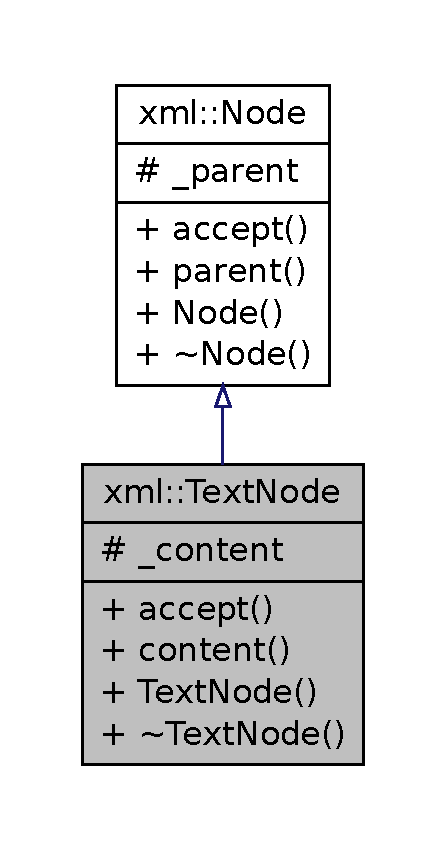
\includegraphics[width=214pt]{classxml_1_1_text_node__inherit__graph}
\end{center}
\end{figure}


Graphe de collaboration de xml::TextNode:\nopagebreak
\begin{figure}[H]
\begin{center}
\leavevmode
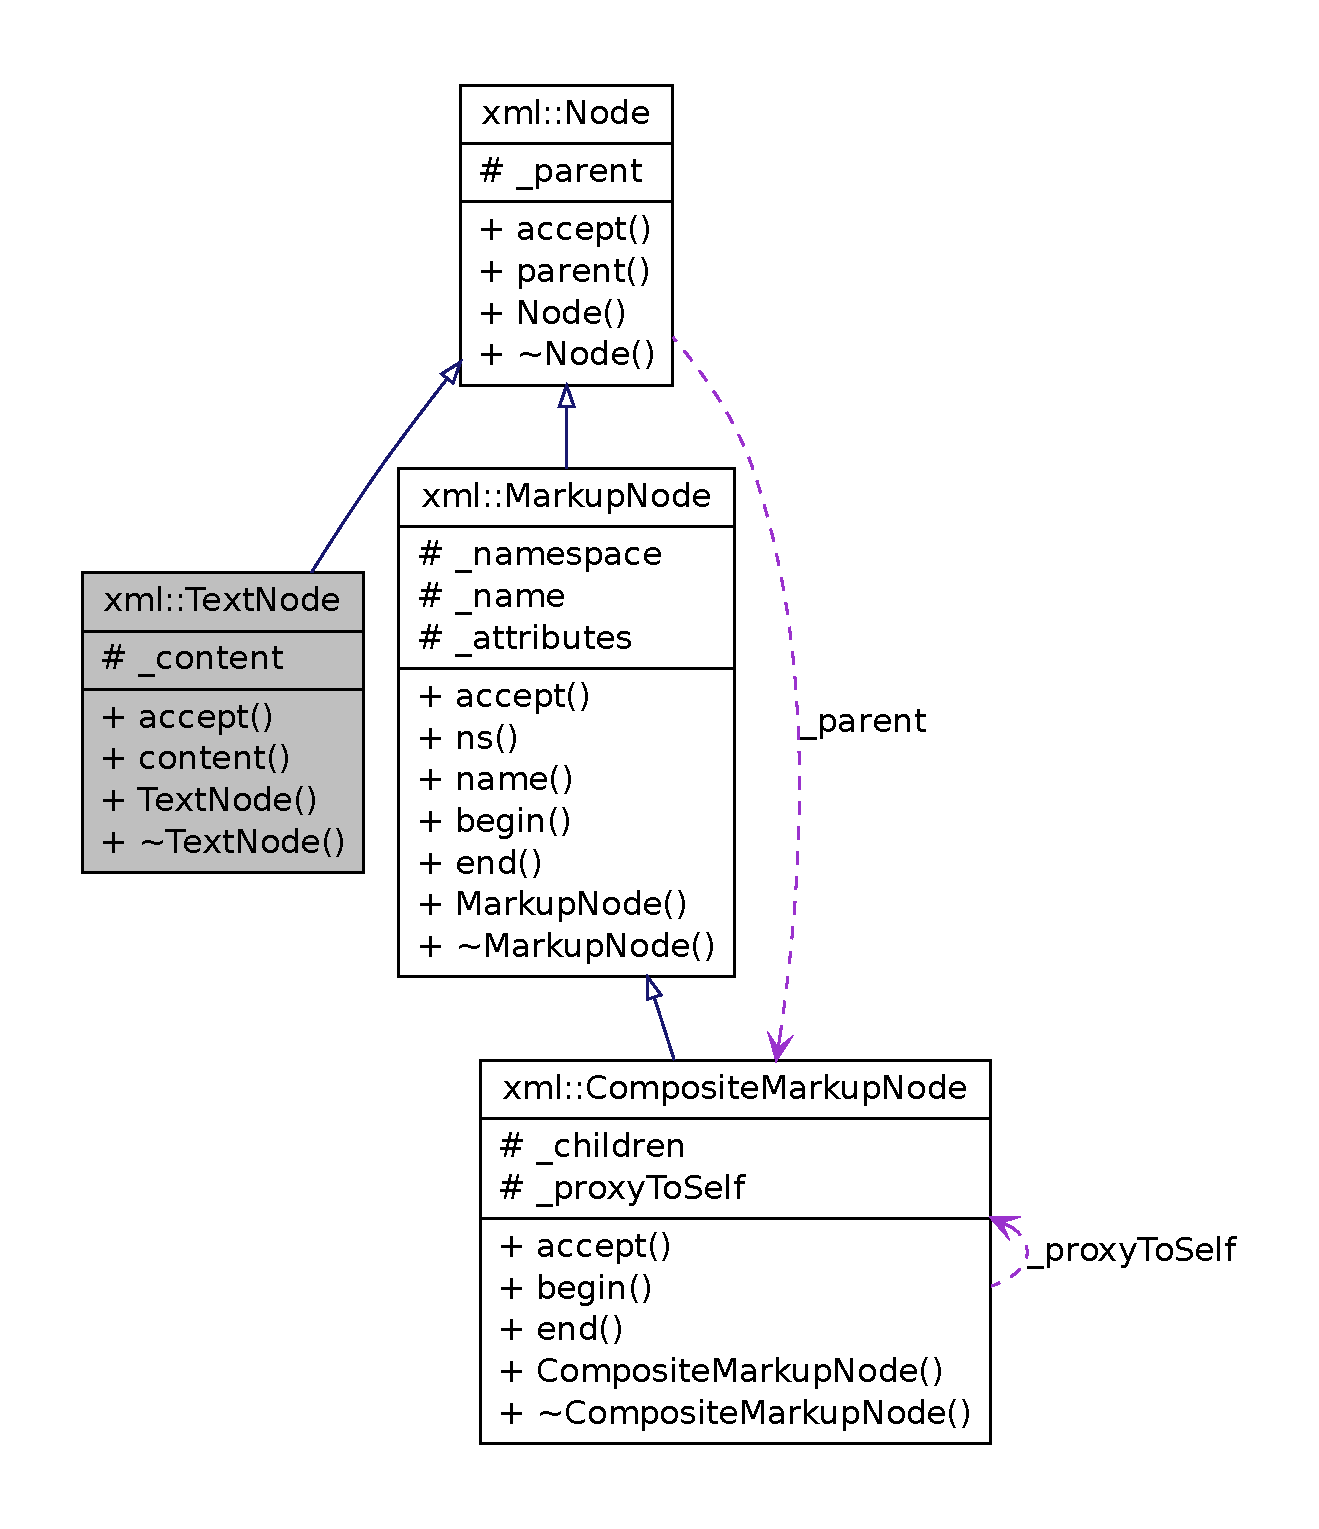
\includegraphics[width=400pt]{classxml_1_1_text_node__coll__graph}
\end{center}
\end{figure}
\subsection*{Fonctions membres publiques}
\begin{DoxyCompactItemize}
\item 
virtual void \hyperlink{classxml_1_1_text_node_ac918f8f74e141690e18cd8e23d174996}{accept} (\hyperlink{classxml_1_1_interface_node_visitor}{InterfaceNodeVisitor} \&visitor) const 
\item 
std::string \hyperlink{classxml_1_1_text_node_a25941b48615a65258cc17d85bc0691d1}{content} () const 
\item 
\hyperlink{classxml_1_1_text_node_aa792bfa28288ba0b52f38215acb1feb0}{TextNode} (\hyperlink{classxml_1_1_composite_markup_node}{CompositeMarkupNode} $\ast$$\ast$parent, const std::string \&content)
\item 
virtual \hyperlink{classxml_1_1_text_node_a631efcd9de6889ba2b8f31e578267d29}{$\sim$TextNode} ()
\end{DoxyCompactItemize}
\subsection*{Attributs protégés}
\begin{DoxyCompactItemize}
\item 
std::string \hyperlink{classxml_1_1_text_node_a1c237e716b3f9fd76569d443d838cd25}{\_\-content}
\end{DoxyCompactItemize}


\subsection{Description détaillée}


Définition à la ligne 25 du fichier TextNode.hh.



\subsection{Documentation des constructeurs et destructeur}
\hypertarget{classxml_1_1_text_node_aa792bfa28288ba0b52f38215acb1feb0}{
\index{xml::TextNode@{xml::TextNode}!TextNode@{TextNode}}
\index{TextNode@{TextNode}!xml::TextNode@{xml::TextNode}}
\subsubsection[{TextNode}]{\setlength{\rightskip}{0pt plus 5cm}xml::TextNode::TextNode (
\begin{DoxyParamCaption}
\item[{{\bf CompositeMarkupNode} $\ast$$\ast$}]{ parent, }
\item[{const std::string \&}]{ content}
\end{DoxyParamCaption}
)}}
\label{classxml_1_1_text_node_aa792bfa28288ba0b52f38215acb1feb0}
\hypertarget{classxml_1_1_text_node_a631efcd9de6889ba2b8f31e578267d29}{
\index{xml::TextNode@{xml::TextNode}!$\sim$TextNode@{$\sim$TextNode}}
\index{$\sim$TextNode@{$\sim$TextNode}!xml::TextNode@{xml::TextNode}}
\subsubsection[{$\sim$TextNode}]{\setlength{\rightskip}{0pt plus 5cm}xml::TextNode::$\sim$TextNode (
\begin{DoxyParamCaption}
{}
\end{DoxyParamCaption}
)\hspace{0.3cm}{\ttfamily  \mbox{[}virtual\mbox{]}}}}
\label{classxml_1_1_text_node_a631efcd9de6889ba2b8f31e578267d29}


Définition à la ligne 53 du fichier TextNode.cpp.



\subsection{Documentation des fonctions membres}
\hypertarget{classxml_1_1_text_node_ac918f8f74e141690e18cd8e23d174996}{
\index{xml::TextNode@{xml::TextNode}!accept@{accept}}
\index{accept@{accept}!xml::TextNode@{xml::TextNode}}
\subsubsection[{accept}]{\setlength{\rightskip}{0pt plus 5cm}void xml::TextNode::accept (
\begin{DoxyParamCaption}
\item[{{\bf InterfaceNodeVisitor} \&}]{ visitor}
\end{DoxyParamCaption}
) const\hspace{0.3cm}{\ttfamily  \mbox{[}virtual\mbox{]}}}}
\label{classxml_1_1_text_node_ac918f8f74e141690e18cd8e23d174996}


Implémente \hyperlink{classxml_1_1_node_a332d84602db92c390e57eeec79c4b02d}{xml::Node}.



Définition à la ligne 32 du fichier TextNode.cpp.



Voici le graphe d'appel pour cette fonction :\nopagebreak
\begin{figure}[H]
\begin{center}
\leavevmode
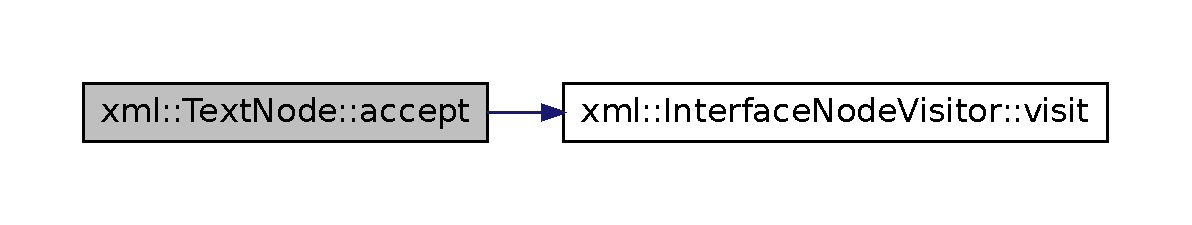
\includegraphics[width=400pt]{classxml_1_1_text_node_ac918f8f74e141690e18cd8e23d174996_cgraph}
\end{center}
\end{figure}


\hypertarget{classxml_1_1_text_node_a25941b48615a65258cc17d85bc0691d1}{
\index{xml::TextNode@{xml::TextNode}!content@{content}}
\index{content@{content}!xml::TextNode@{xml::TextNode}}
\subsubsection[{content}]{\setlength{\rightskip}{0pt plus 5cm}string xml::TextNode::content (
\begin{DoxyParamCaption}
{}
\end{DoxyParamCaption}
) const}}
\label{classxml_1_1_text_node_a25941b48615a65258cc17d85bc0691d1}


Définition à la ligne 37 du fichier TextNode.cpp.



Voici le graphe d'appel pour cette fonction :
\nopagebreak
\begin{figure}[H]
\begin{center}
\leavevmode
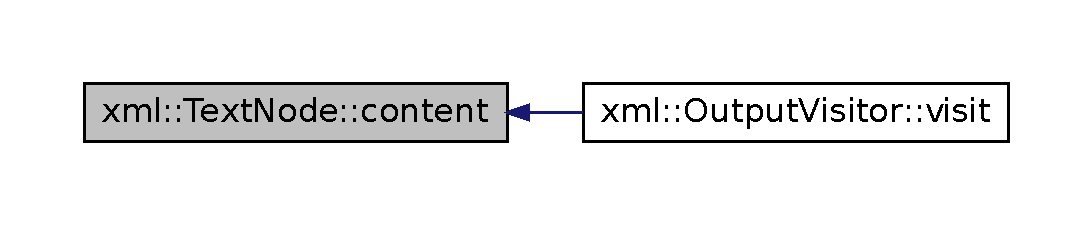
\includegraphics[width=400pt]{classxml_1_1_text_node_a25941b48615a65258cc17d85bc0691d1_icgraph}
\end{center}
\end{figure}




\subsection{Documentation des données membres}
\hypertarget{classxml_1_1_text_node_a1c237e716b3f9fd76569d443d838cd25}{
\index{xml::TextNode@{xml::TextNode}!\_\-content@{\_\-content}}
\index{\_\-content@{\_\-content}!xml::TextNode@{xml::TextNode}}
\subsubsection[{\_\-content}]{\setlength{\rightskip}{0pt plus 5cm}std::string {\bf xml::TextNode::\_\-content}\hspace{0.3cm}{\ttfamily  \mbox{[}protected\mbox{]}}}}
\label{classxml_1_1_text_node_a1c237e716b3f9fd76569d443d838cd25}


Définition à la ligne 62 du fichier TextNode.hh.



La documentation de cette classe a été générée à partir des fichiers suivants :\begin{DoxyCompactItemize}
\item 
src/\hyperlink{_text_node_8hh}{TextNode.hh}\item 
src/\hyperlink{_text_node_8cpp}{TextNode.cpp}\end{DoxyCompactItemize}

\chapter{Documentation des fichiers}
\hypertarget{_composite_markup_node_8cpp}{
\section{Référence du fichier src/CompositeMarkupNode.cpp}
\label{_composite_markup_node_8cpp}\index{src/CompositeMarkupNode.cpp@{src/CompositeMarkupNode.cpp}}
}
{\ttfamily \#include $<$string$>$}\par
{\ttfamily \#include \char`\"{}CompositeMarkupNode.hh\char`\"{}}\par
Graphe des dépendances par inclusion de CompositeMarkupNode.cpp:
\nopagebreak
\begin{figure}[H]
\begin{center}
\leavevmode
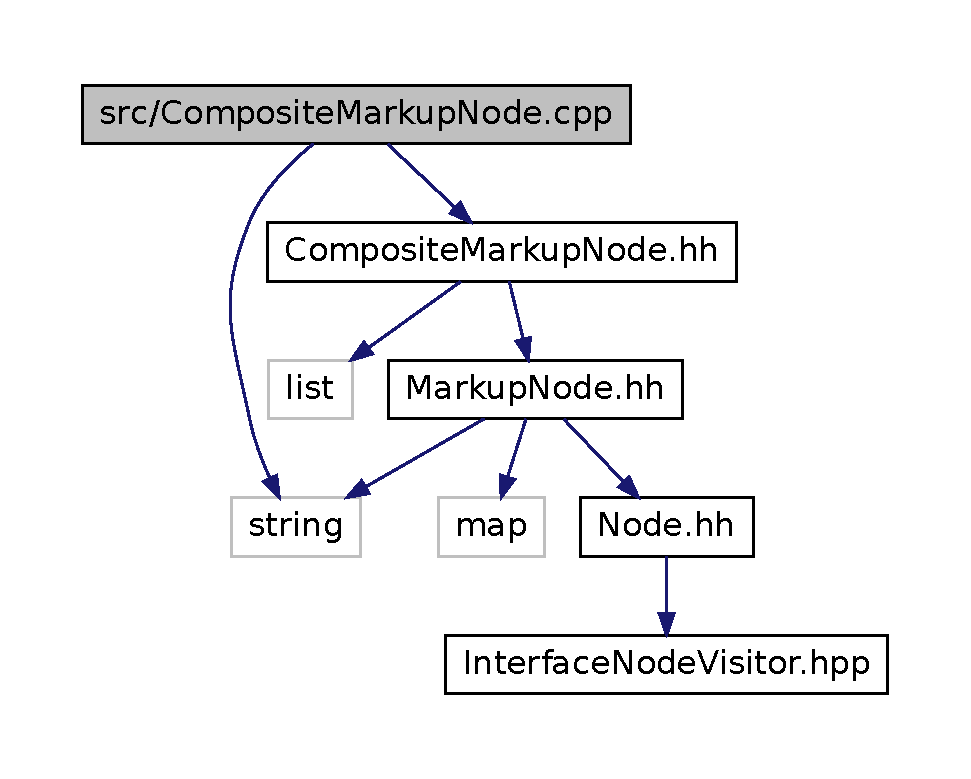
\includegraphics[width=400pt]{_composite_markup_node_8cpp__incl}
\end{center}
\end{figure}
\subsection*{Espaces de nommage}
\begin{DoxyCompactItemize}
\item 
namespace \hyperlink{namespacexml}{xml}
\end{DoxyCompactItemize}

\hypertarget{_composite_markup_node_8hh}{
\section{Référence du fichier src/CompositeMarkupNode.hh}
\label{_composite_markup_node_8hh}\index{src/CompositeMarkupNode.hh@{src/CompositeMarkupNode.hh}}
}
{\ttfamily \#include $<$list$>$}\par
{\ttfamily \#include \char`\"{}MarkupNode.hh\char`\"{}}\par
Graphe des dépendances par inclusion de CompositeMarkupNode.hh:
\nopagebreak
\begin{figure}[H]
\begin{center}
\leavevmode
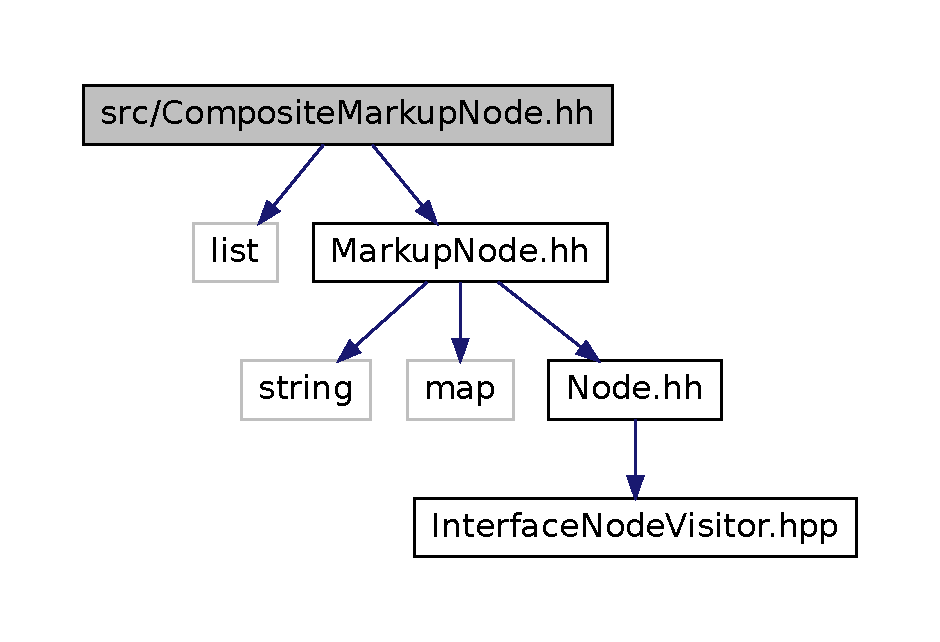
\includegraphics[width=400pt]{_composite_markup_node_8hh__incl}
\end{center}
\end{figure}
Ce graphe montre quels fichiers incluent directement ou indirectement ce fichier :
\nopagebreak
\begin{figure}[H]
\begin{center}
\leavevmode
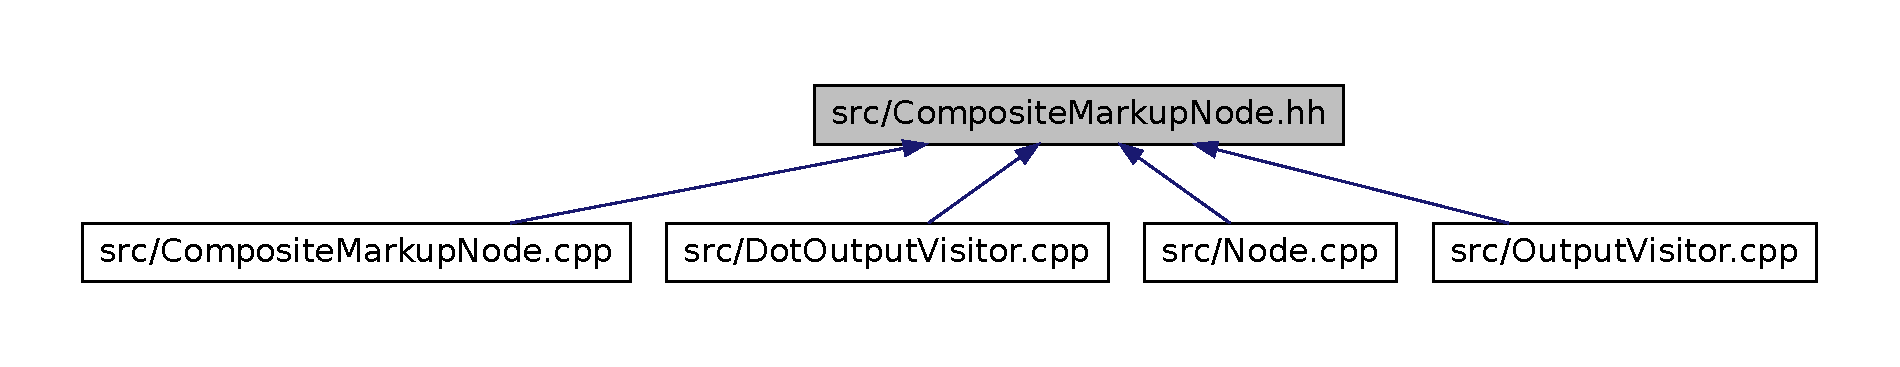
\includegraphics[width=400pt]{_composite_markup_node_8hh__dep__incl}
\end{center}
\end{figure}
\subsection*{Classes}
\begin{DoxyCompactItemize}
\item 
class \hyperlink{classxml_1_1_composite_markup_node}{xml::CompositeMarkupNode}
\end{DoxyCompactItemize}
\subsection*{Espaces de nommage}
\begin{DoxyCompactItemize}
\item 
namespace \hyperlink{namespacexml}{xml}
\end{DoxyCompactItemize}

\hypertarget{_dot_output_visitor_8cpp}{
\section{Référence du fichier src/DotOutputVisitor.cpp}
\label{_dot_output_visitor_8cpp}\index{src/DotOutputVisitor.cpp@{src/DotOutputVisitor.cpp}}
}
{\ttfamily \#include $<$iostream$>$}\par
{\ttfamily \#include $<$iomanip$>$}\par
{\ttfamily \#include \char`\"{}DotOutputVisitor.hh\char`\"{}}\par
{\ttfamily \#include \char`\"{}TextNode.hh\char`\"{}}\par
{\ttfamily \#include \char`\"{}MarkupNode.hh\char`\"{}}\par
{\ttfamily \#include \char`\"{}CompositeMarkupNode.hh\char`\"{}}\par
Graphe des dépendances par inclusion de DotOutputVisitor.cpp:
\nopagebreak
\begin{figure}[H]
\begin{center}
\leavevmode
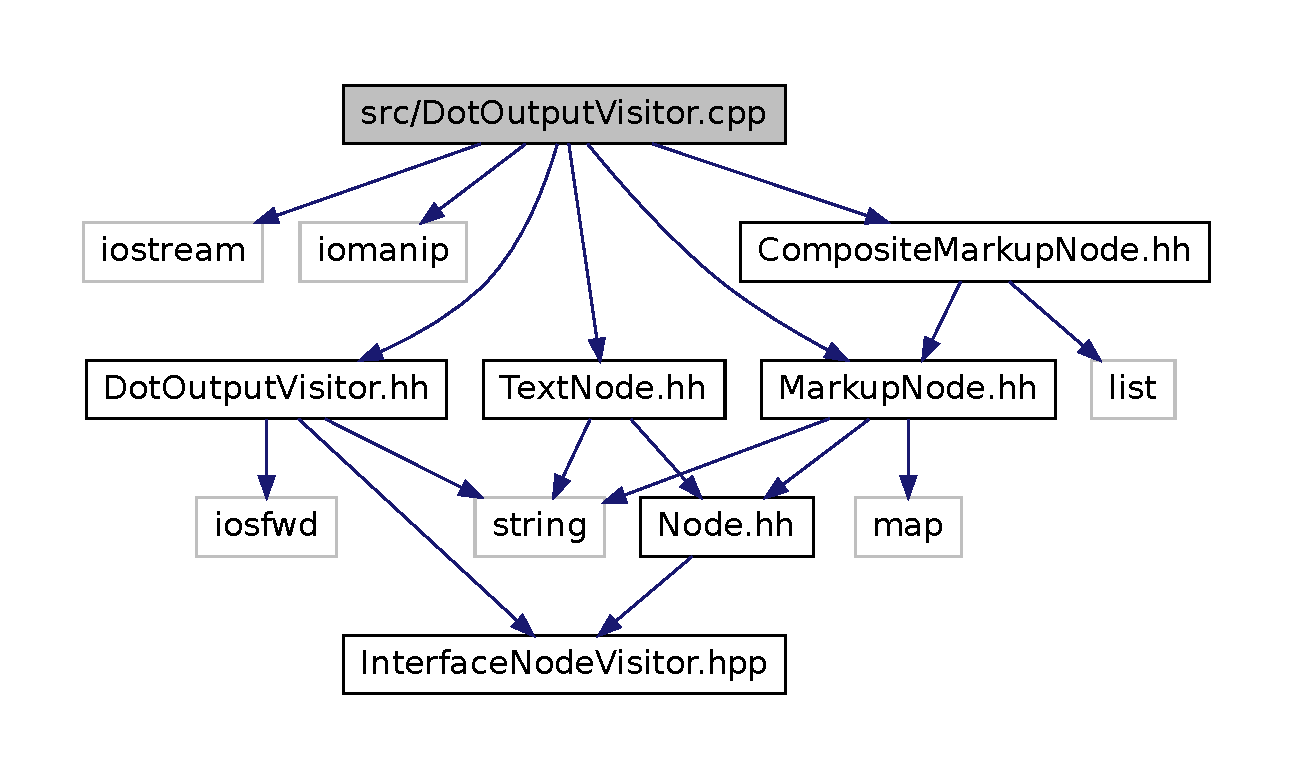
\includegraphics[width=400pt]{_dot_output_visitor_8cpp__incl}
\end{center}
\end{figure}
\subsection*{Espaces de nommage}
\begin{DoxyCompactItemize}
\item 
namespace \hyperlink{namespacexml}{xml}
\end{DoxyCompactItemize}

\hypertarget{_dot_output_visitor_8hh}{
\section{Référence du fichier src/DotOutputVisitor.hh}
\label{_dot_output_visitor_8hh}\index{src/DotOutputVisitor.hh@{src/DotOutputVisitor.hh}}
}
{\ttfamily \#include $<$iosfwd$>$}\par
{\ttfamily \#include $<$string$>$}\par
{\ttfamily \#include \char`\"{}InterfaceNodeVisitor.hpp\char`\"{}}\par
Graphe des dépendances par inclusion de DotOutputVisitor.hh:\nopagebreak
\begin{figure}[H]
\begin{center}
\leavevmode
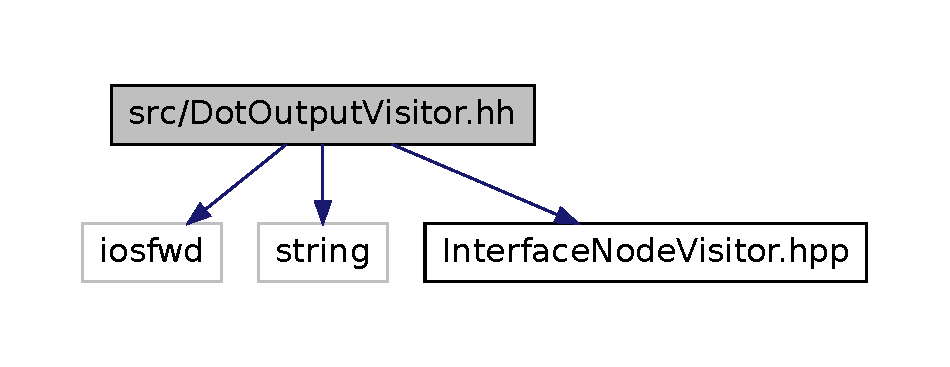
\includegraphics[width=400pt]{_dot_output_visitor_8hh__incl}
\end{center}
\end{figure}
Ce graphe montre quels fichiers incluent directement ou indirectement ce fichier :\nopagebreak
\begin{figure}[H]
\begin{center}
\leavevmode
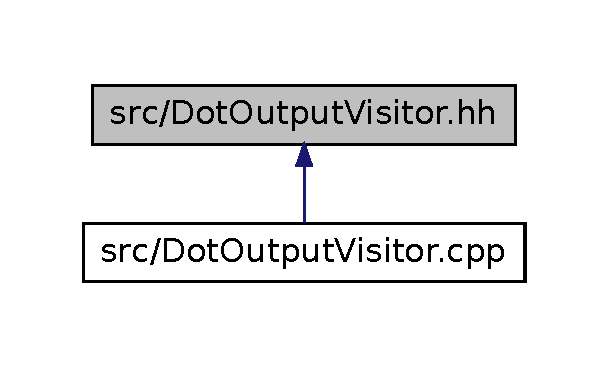
\includegraphics[width=292pt]{_dot_output_visitor_8hh__dep__incl}
\end{center}
\end{figure}
\subsection*{Classes}
\begin{DoxyCompactItemize}
\item 
class \hyperlink{classxml_1_1_dot_output_visitor}{xml::DotOutputVisitor}
\end{DoxyCompactItemize}
\subsection*{Espaces de nommage}
\begin{DoxyCompactItemize}
\item 
namespace \hyperlink{namespacexml}{xml}
\end{DoxyCompactItemize}

\hypertarget{_interface_node_visitor_8hpp}{
\section{Référence du fichier src/InterfaceNodeVisitor.hpp}
\label{_interface_node_visitor_8hpp}\index{src/InterfaceNodeVisitor.hpp@{src/InterfaceNodeVisitor.hpp}}
}
Ce graphe montre quels fichiers incluent directement ou indirectement ce fichier :
\nopagebreak
\begin{figure}[H]
\begin{center}
\leavevmode
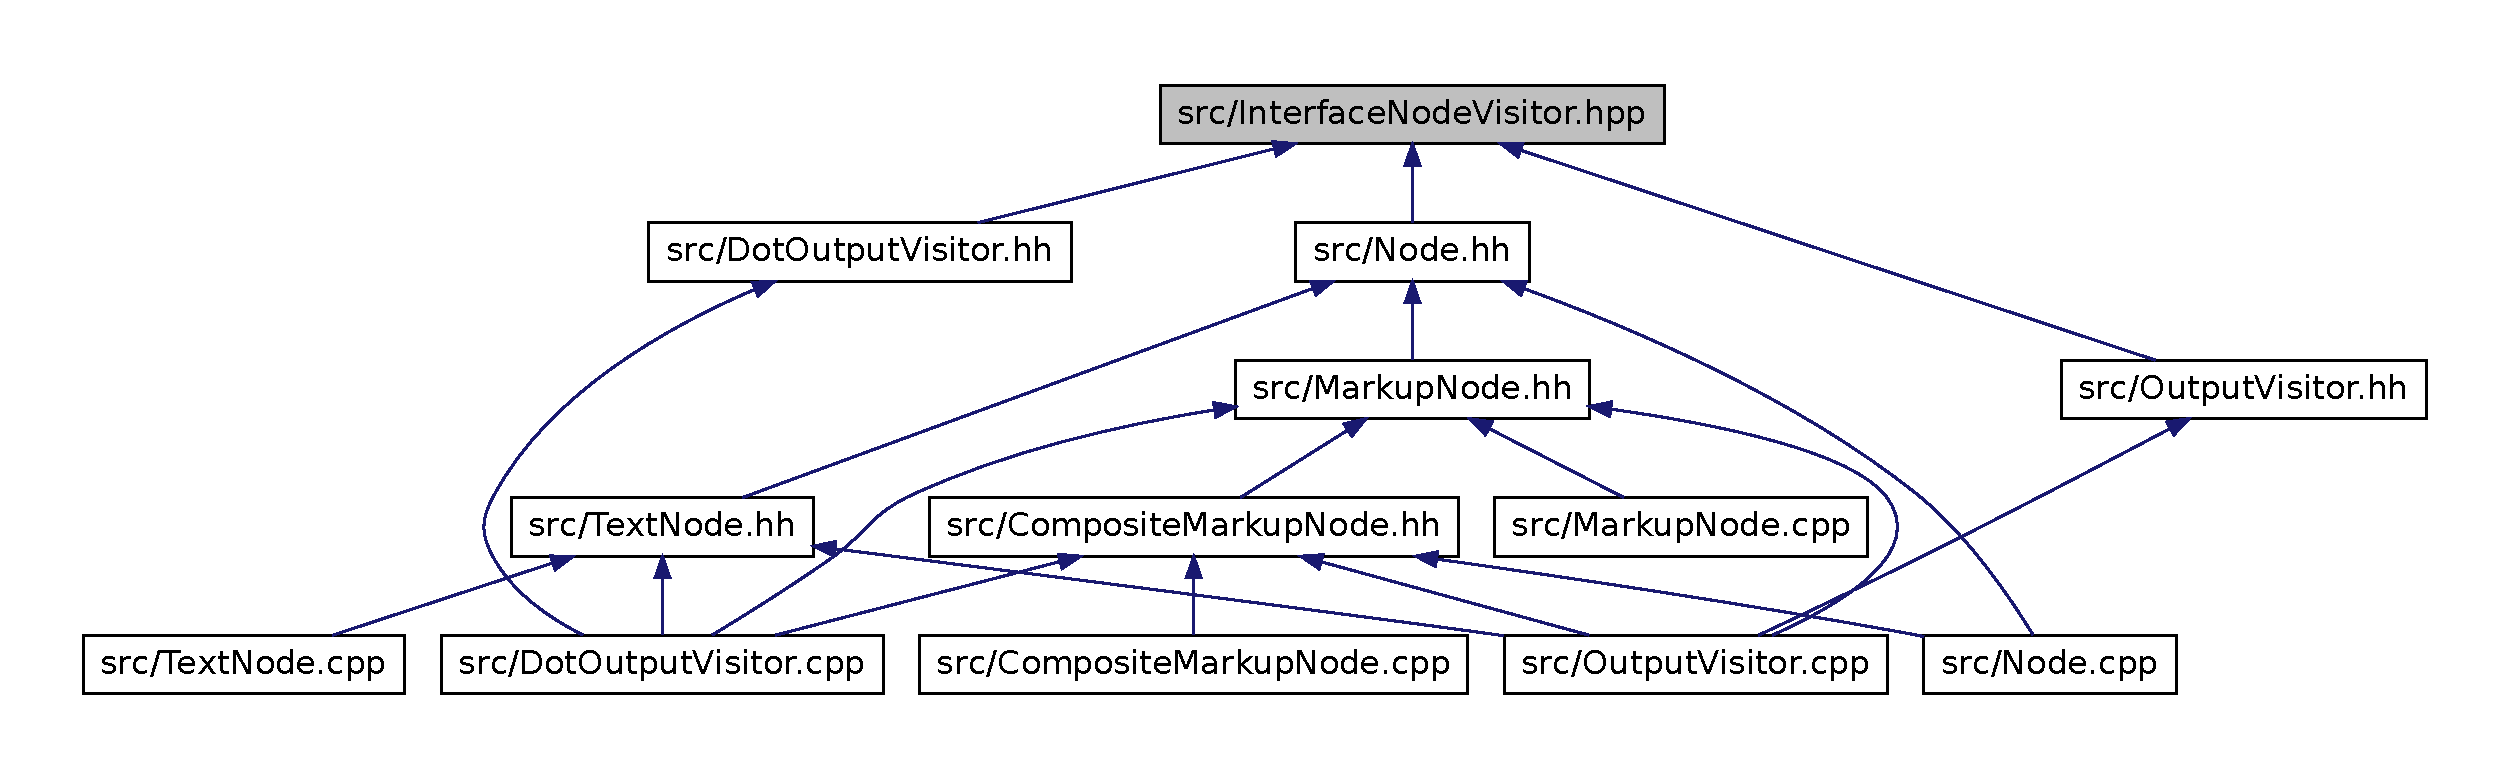
\includegraphics[width=400pt]{_interface_node_visitor_8hpp__dep__incl}
\end{center}
\end{figure}
\subsection*{Classes}
\begin{DoxyCompactItemize}
\item 
class \hyperlink{classxml_1_1_interface_node_visitor}{xml::InterfaceNodeVisitor}
\end{DoxyCompactItemize}
\subsection*{Espaces de nommage}
\begin{DoxyCompactItemize}
\item 
namespace \hyperlink{namespacexml}{xml}
\end{DoxyCompactItemize}

\hypertarget{_markup_node_8cpp}{
\section{Référence du fichier src/MarkupNode.cpp}
\label{_markup_node_8cpp}\index{src/MarkupNode.cpp@{src/MarkupNode.cpp}}
}
{\ttfamily \#include $<$iostream$>$}\par
{\ttfamily \#include \char`\"{}MarkupNode.hh\char`\"{}}\par
Graphe des dépendances par inclusion de MarkupNode.cpp:
\nopagebreak
\begin{figure}[H]
\begin{center}
\leavevmode
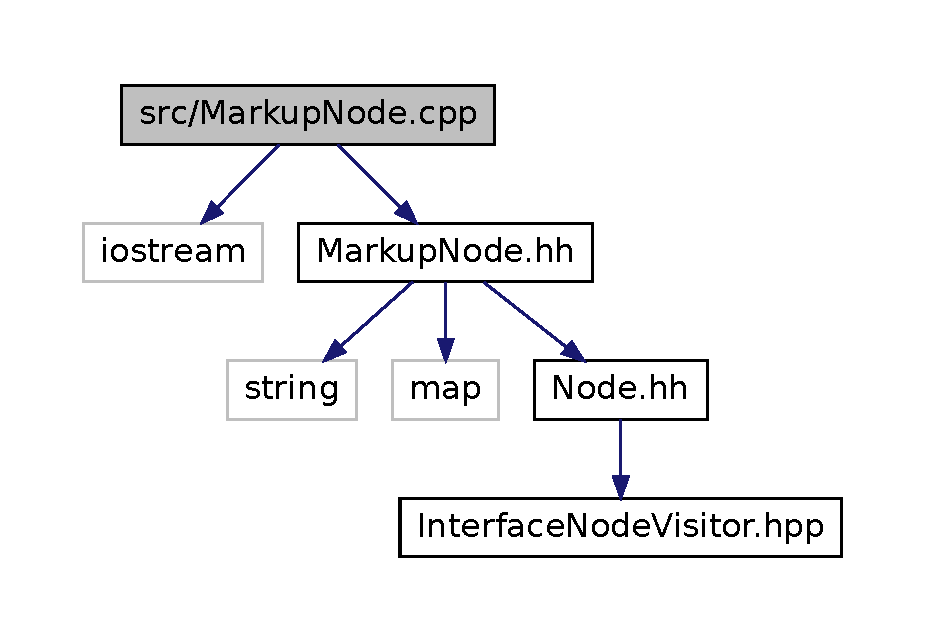
\includegraphics[width=400pt]{_markup_node_8cpp__incl}
\end{center}
\end{figure}
\subsection*{Espaces de nommage}
\begin{DoxyCompactItemize}
\item 
namespace \hyperlink{namespacexml}{xml}
\end{DoxyCompactItemize}

\hypertarget{_markup_node_8hh}{
\section{Référence du fichier src/MarkupNode.hh}
\label{_markup_node_8hh}\index{src/MarkupNode.hh@{src/MarkupNode.hh}}
}
{\ttfamily \#include $<$string$>$}\par
{\ttfamily \#include $<$map$>$}\par
{\ttfamily \#include \char`\"{}Node.hh\char`\"{}}\par
Graphe des dépendances par inclusion de MarkupNode.hh:
\nopagebreak
\begin{figure}[H]
\begin{center}
\leavevmode
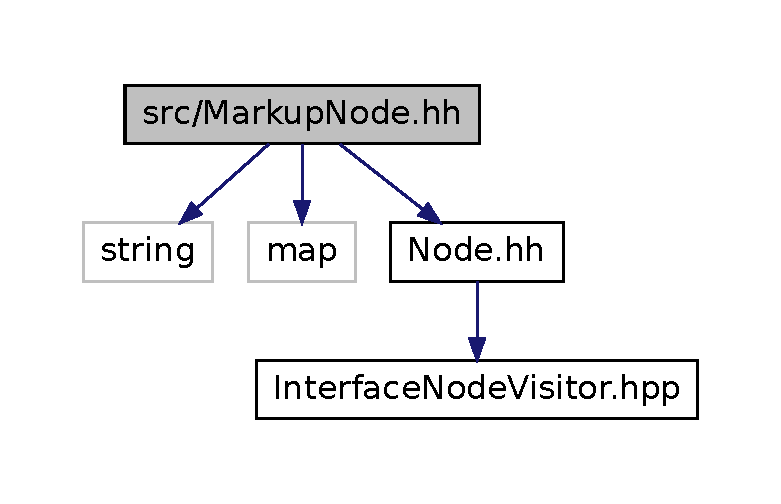
\includegraphics[width=375pt]{_markup_node_8hh__incl}
\end{center}
\end{figure}
Ce graphe montre quels fichiers incluent directement ou indirectement ce fichier :
\nopagebreak
\begin{figure}[H]
\begin{center}
\leavevmode
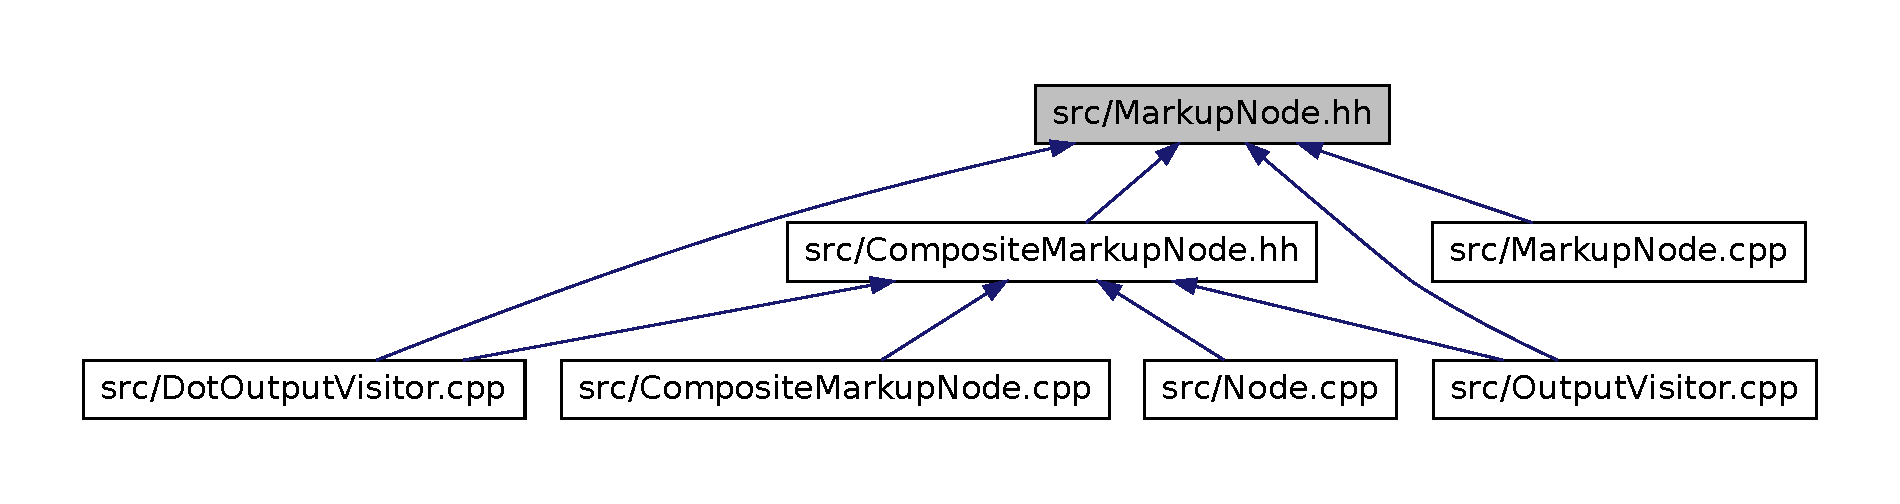
\includegraphics[width=400pt]{_markup_node_8hh__dep__incl}
\end{center}
\end{figure}
\subsection*{Classes}
\begin{DoxyCompactItemize}
\item 
class \hyperlink{classxml_1_1_markup_node}{xml::MarkupNode}
\end{DoxyCompactItemize}
\subsection*{Espaces de nommage}
\begin{DoxyCompactItemize}
\item 
namespace \hyperlink{namespacexml}{xml}
\end{DoxyCompactItemize}

\hypertarget{_node_8cpp}{
\section{Référence du fichier src/Node.cpp}
\label{_node_8cpp}\index{src/Node.cpp@{src/Node.cpp}}
}
{\ttfamily \#include \char`\"{}Node.hh\char`\"{}}\par
{\ttfamily \#include \char`\"{}CompositeMarkupNode.hh\char`\"{}}\par
Graphe des dépendances par inclusion de Node.cpp:\nopagebreak
\begin{figure}[H]
\begin{center}
\leavevmode
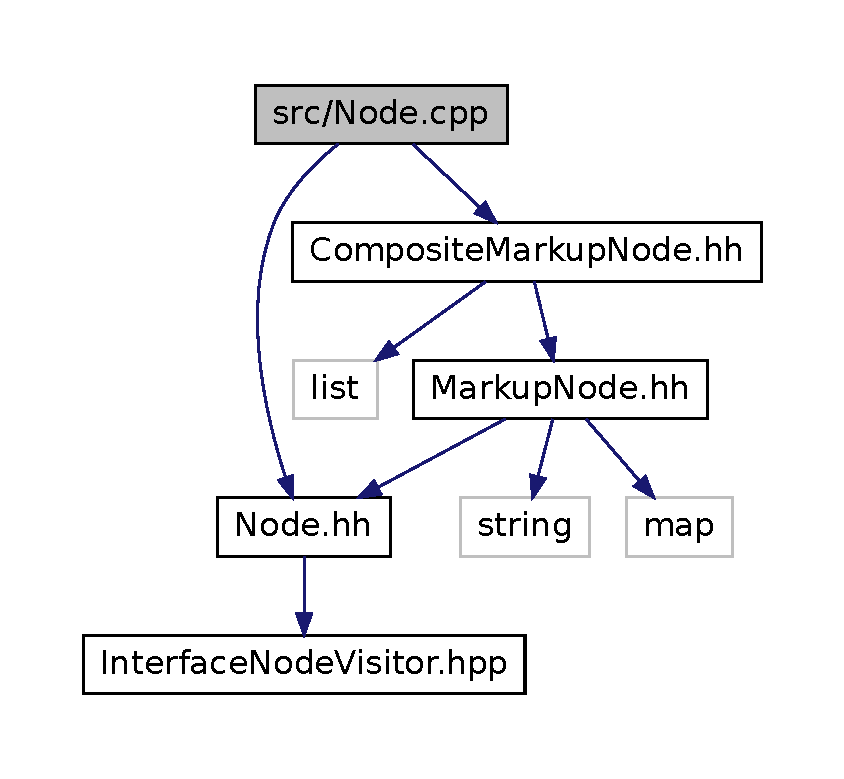
\includegraphics[width=400pt]{_node_8cpp__incl}
\end{center}
\end{figure}
\subsection*{Espaces de nommage}
\begin{DoxyCompactItemize}
\item 
namespace \hyperlink{namespacexml}{xml}
\end{DoxyCompactItemize}

\hypertarget{_node_8hh}{
\section{Référence du fichier src/Node.hh}
\label{_node_8hh}\index{src/Node.hh@{src/Node.hh}}
}
{\ttfamily \#include \char`\"{}InterfaceNodeVisitor.hpp\char`\"{}}\par
Graphe des dépendances par inclusion de Node.hh:
\nopagebreak
\begin{figure}[H]
\begin{center}
\leavevmode
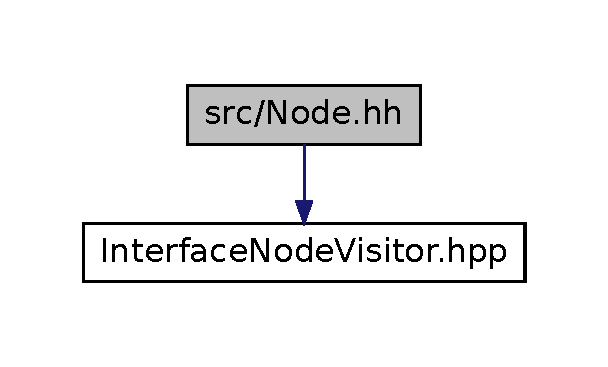
\includegraphics[width=292pt]{_node_8hh__incl}
\end{center}
\end{figure}
Ce graphe montre quels fichiers incluent directement ou indirectement ce fichier :
\nopagebreak
\begin{figure}[H]
\begin{center}
\leavevmode
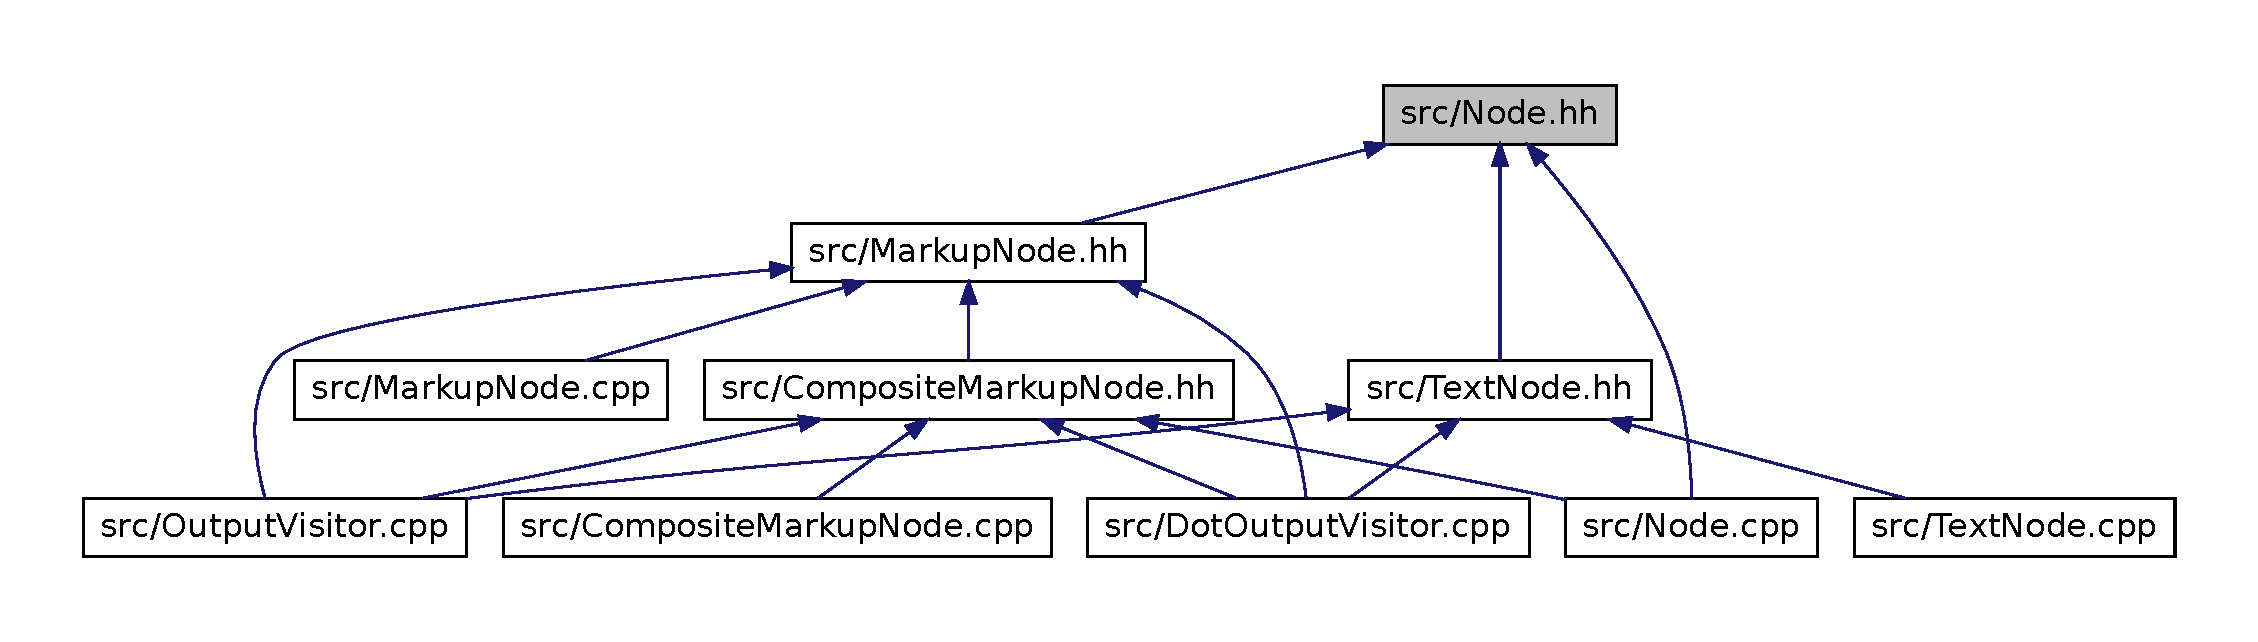
\includegraphics[width=400pt]{_node_8hh__dep__incl}
\end{center}
\end{figure}
\subsection*{Classes}
\begin{DoxyCompactItemize}
\item 
class \hyperlink{classxml_1_1_node}{xml::Node}
\end{DoxyCompactItemize}
\subsection*{Espaces de nommage}
\begin{DoxyCompactItemize}
\item 
namespace \hyperlink{namespacexml}{xml}
\end{DoxyCompactItemize}

\hypertarget{_output_visitor_8cpp}{
\section{Référence du fichier src/OutputVisitor.cpp}
\label{_output_visitor_8cpp}\index{src/OutputVisitor.cpp@{src/OutputVisitor.cpp}}
}
{\ttfamily \#include $<$iostream$>$}\par
{\ttfamily \#include $<$iomanip$>$}\par
{\ttfamily \#include \char`\"{}OutputVisitor.hh\char`\"{}}\par
{\ttfamily \#include \char`\"{}TextNode.hh\char`\"{}}\par
{\ttfamily \#include \char`\"{}MarkupNode.hh\char`\"{}}\par
{\ttfamily \#include \char`\"{}CompositeMarkupNode.hh\char`\"{}}\par
Graphe des dépendances par inclusion de OutputVisitor.cpp:
\nopagebreak
\begin{figure}[H]
\begin{center}
\leavevmode
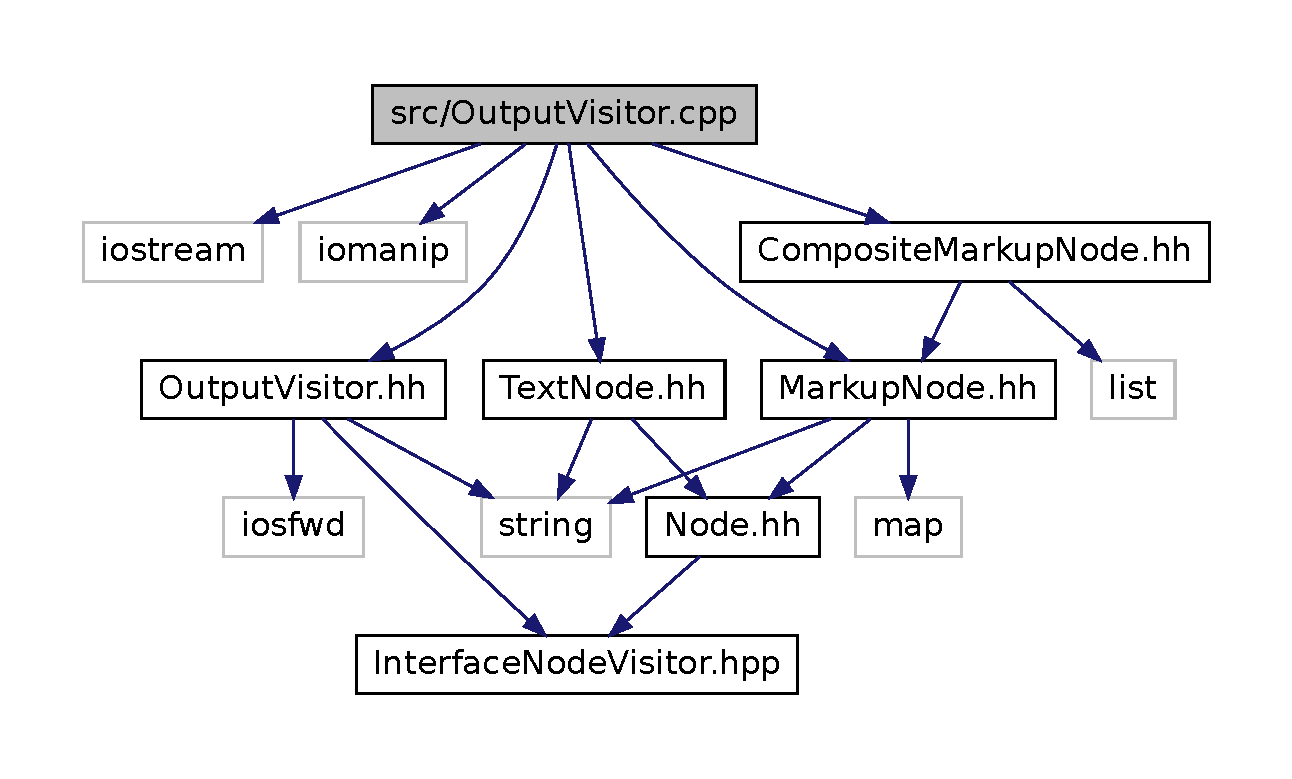
\includegraphics[width=400pt]{_output_visitor_8cpp__incl}
\end{center}
\end{figure}
\subsection*{Espaces de nommage}
\begin{DoxyCompactItemize}
\item 
namespace \hyperlink{namespacexml}{xml}
\end{DoxyCompactItemize}

\hypertarget{_output_visitor_8hh}{
\section{Référence du fichier src/OutputVisitor.hh}
\label{_output_visitor_8hh}\index{src/OutputVisitor.hh@{src/OutputVisitor.hh}}
}
{\ttfamily \#include $<$iosfwd$>$}\par
{\ttfamily \#include $<$string$>$}\par
{\ttfamily \#include \char`\"{}InterfaceNodeVisitor.hpp\char`\"{}}\par
Graphe des dépendances par inclusion de OutputVisitor.hh:
\nopagebreak
\begin{figure}[H]
\begin{center}
\leavevmode
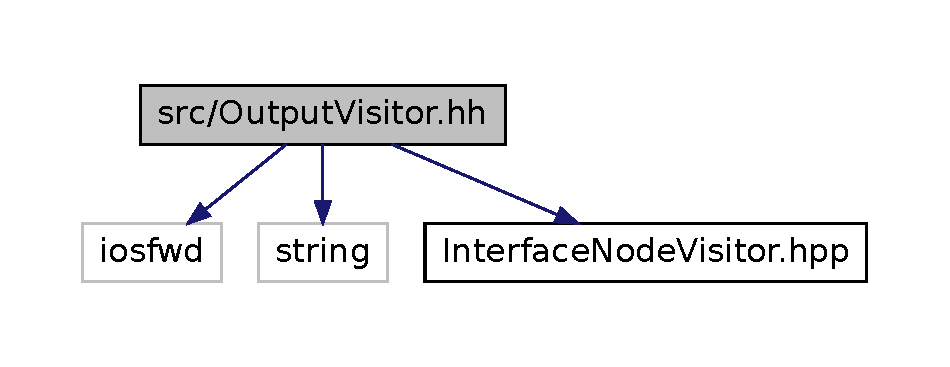
\includegraphics[width=400pt]{_output_visitor_8hh__incl}
\end{center}
\end{figure}
Ce graphe montre quels fichiers incluent directement ou indirectement ce fichier :
\nopagebreak
\begin{figure}[H]
\begin{center}
\leavevmode
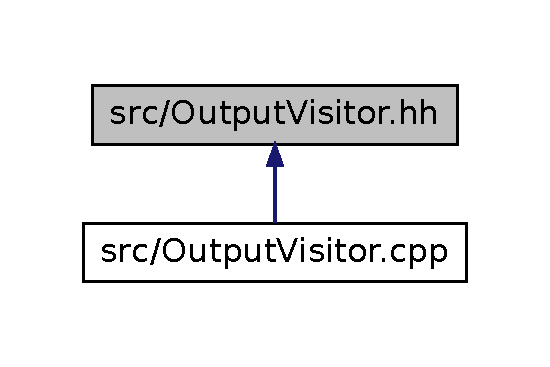
\includegraphics[width=264pt]{_output_visitor_8hh__dep__incl}
\end{center}
\end{figure}
\subsection*{Classes}
\begin{DoxyCompactItemize}
\item 
class \hyperlink{classxml_1_1_output_visitor}{xml::OutputVisitor}
\end{DoxyCompactItemize}
\subsection*{Espaces de nommage}
\begin{DoxyCompactItemize}
\item 
namespace \hyperlink{namespacexml}{xml}
\end{DoxyCompactItemize}

\hypertarget{_text_node_8cpp}{
\section{Référence du fichier src/TextNode.cpp}
\label{_text_node_8cpp}\index{src/TextNode.cpp@{src/TextNode.cpp}}
}
{\ttfamily \#include $<$string$>$}\par
{\ttfamily \#include \char`\"{}TextNode.hh\char`\"{}}\par
Graphe des dépendances par inclusion de TextNode.cpp:\nopagebreak
\begin{figure}[H]
\begin{center}
\leavevmode
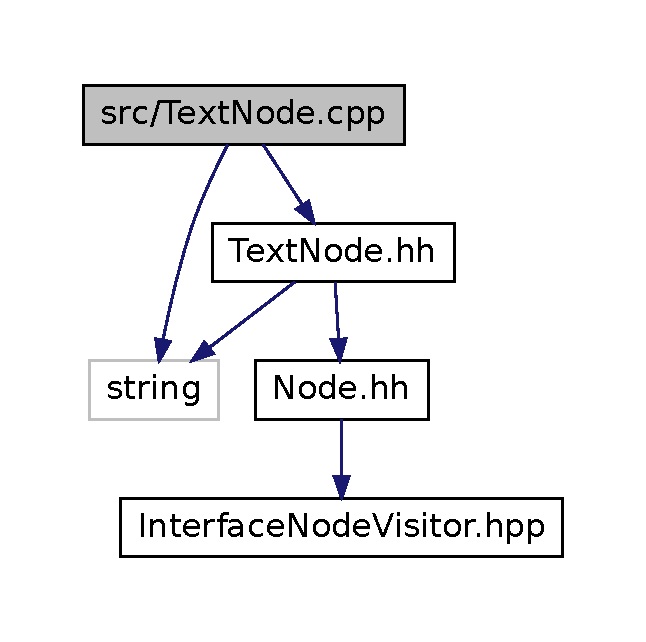
\includegraphics[width=310pt]{_text_node_8cpp__incl}
\end{center}
\end{figure}
\subsection*{Espaces de nommage}
\begin{DoxyCompactItemize}
\item 
namespace \hyperlink{namespacexml}{xml}
\end{DoxyCompactItemize}

\hypertarget{_text_node_8hh}{
\section{Référence du fichier src/TextNode.hh}
\label{_text_node_8hh}\index{src/TextNode.hh@{src/TextNode.hh}}
}
{\ttfamily \#include $<$string$>$}\par
{\ttfamily \#include \char`\"{}Node.hh\char`\"{}}\par
Graphe des dépendances par inclusion de TextNode.hh:\nopagebreak
\begin{figure}[H]
\begin{center}
\leavevmode
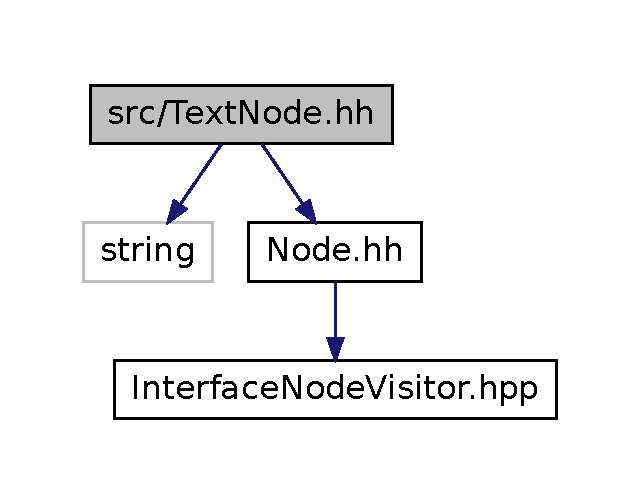
\includegraphics[width=307pt]{_text_node_8hh__incl}
\end{center}
\end{figure}
Ce graphe montre quels fichiers incluent directement ou indirectement ce fichier :\nopagebreak
\begin{figure}[H]
\begin{center}
\leavevmode
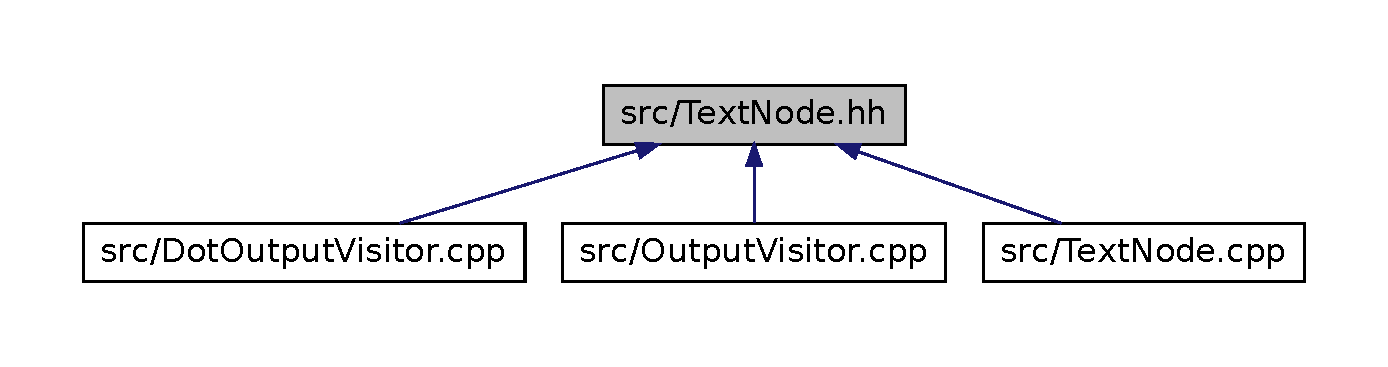
\includegraphics[width=400pt]{_text_node_8hh__dep__incl}
\end{center}
\end{figure}
\subsection*{Classes}
\begin{DoxyCompactItemize}
\item 
class \hyperlink{classxml_1_1_text_node}{xml::TextNode}
\end{DoxyCompactItemize}
\subsection*{Espaces de nommage}
\begin{DoxyCompactItemize}
\item 
namespace \hyperlink{namespacexml}{xml}
\end{DoxyCompactItemize}

\printindex
\end{document}
